%
% MJ Meintjes thys@postino.up.ac.za 1997 June
% Department of Electrical&Electronic Engineering
% Biogroup
% University of Pretoria
% South Africa
%
% 97/06/26 Language change, primary design&latex skeletal
% implementation
%

\documentclass[a4paper,12pt]{report}
\usepackage[english]{babel}
\usepackage{graphicx}
\usepackage{psfrag}
\usepackage{color}
\usepackage{varioref}


\begin{document}
\title{\bf{AN INVESTIGATION INTO THE FEASIBILITY OF AN ACTIVE ELECTRODE
		EEG DATA ACQUISITION SYSTEM}}
\author{by\\M.J Meintjes \\ Submitted in partial fulfillment for the degree\\
		Master of Engineering (Bio--Engineering)\\
		in the\\
		Faculty of Engineering\\
		\\
		UNIVERSITY OF PRETORIA}
\date{}
\maketitle
\abstract{

This report documents the design and implementation of a
active--electrode EEG data--acquisition system. The system design is
logically and physically separated into independent functional
modules. Each module is designed and implemented with the reduction of
the effects of environmental and system noise as primary goal. Various
techniques are employed to prevent the degradation of EEG signals by
both external and internal noise sources within all system
modules. The primary goal of the system is to achieve the highest
possible degree of usability within the lowest possible noise
budget. Quantitative estimates of acceptable noise levels are used to
calculate the maximum level of permissible system noise. This noise
budget is primarily spent on the signal acquisition modules in an
effort to enhance the level of system usability.}


\tableofcontents
\newpage
\listoffigures
\newpage
\listoftables
\newpage

\pagestyle{headings}

\chapter{Introduction}
%Thys Meintjes for M.Eng 
%introduction.tex
%included in skripsie.tex


\section{Rationale}

The electroencephalogram (EEG) is a recording of the gross electrical
activity of the brain as measured on the scalp surface. The EEG signal
measured between points on the scalp is the sum of all neuronal
electrical activity in the vicinity of the measuring electrode
conducted to the area where the electrode resides.

The aim of brain research and the subsequent recording of EEG signals
is to understand the relationship between human brain activity and
human perception, cognition and goal directed action
\cite{human}. Various techniques involving stimulated brain responses
are routinely applied in clinical practice and research
environments. These include visual, audio and tactile evoked
potentials. Of these the visual evoked potential is the most widely
used and best understood phenomenon. Diagnostic techniques have been
developed using the visual evoked potential as primary investigative
tool.

The EEG can be used as a parameter in clinical practice for the
analysis and diagnosis of various central nervous system related
pathologies in both human and animal subjects. Electroencephalograms
are used in neurology and psychiatry, mainly to help diagnose diseases
of the brain, such as epilepsy (convulsions caused by a chaotic
activity of neurons), sleep disorders and brain
tumors\footnote{http://www.epub.org.br/cm/n03/tecnologia/eeg.htm}. Knowledge
obtained from EEG data is of a phenomenological nature and usually
relies on the visual analysis of a EEG.

The exact source of various EEG signal artifacts is a subject of
continuous investigation.


In order to measure Bio-electric signals it is necessary to use
electrodes. EEG's are traditionally obtained by using standard gold or
silver surface electrodes with a conductive paste. Since the human
skin resistance varies between 10-100~k$\Omega$
\cite{active-electrode-ca} the potential derived with traditional
surface electrodes is affected by the electrode-skin resistance. The
main cause of skin resistance is the stratum granulosum layer forming
the human skin surface. In order to reduce skin resistance the stratum
granulosum is usually removed with a abrading paste. A conductive
electrode paste is applied to ensure a stable low impedance conductive
path between the electrode and skin surface.

Most recording artifacts and loss of data are directly attributed to
problems associated with the electrode and its application. By
negating the voltage dividing effect of the skin surface the need of a
low-impedance signal path and the associated preparation phase is
circumvented. The effect of skin resistance is negligible if the
electrode input impedance is significantly larger than the skin
resistance. This condition can be satisfied by using a active device
in the realization of the electrode. By replacing the traditional wet
electrodes with dry active electrodes the process of skin preparation
can be eliminated. Eliminating skin preparation and the need for
electrode paste significantly enhances the usability and ergonomic
acceptability of a EEG data acquisition system.


The successful elimination of the time and comfort constraints
introduced by traditional EEG electrode preparation and application
suggests various new application fields. Possible applications range
from enhanced computer interface designs to direct applications in the
rehabilitation engineering field such as appliance control interfaces
for the physically disabled.


\section{System overview}
This report documents the design and implementation of a active
electrode based EEG data--acquisition system. The system forges a path
between the opposing constraints of user--friendliness and signal
quality. This contention exists primarily due to the fact that
extensive skin preparations are needed before EEG recordings may be
attempted.

The author will attempt to demonstrate that the traditional
preparation phase may skipped without adversely affecting EEG signal
quality by applying active electrodes in stead of traditional passive
electrodes.


\begin{figure}[h]
		\psfrag{Signal}[][]{Signal}
		\psfrag{Acquisition}[][]{Acquisition}
		\psfrag{low-level}[][]{Low-level}
		\psfrag{signal}[][]{signal}
		\psfrag{processing}[][]{Processing}
		\psfrag{Conversion}[][]{Conversion}
		\psfrag{Display}[][]{Display}
		\psfrag{High-level}[][]{High-level}
        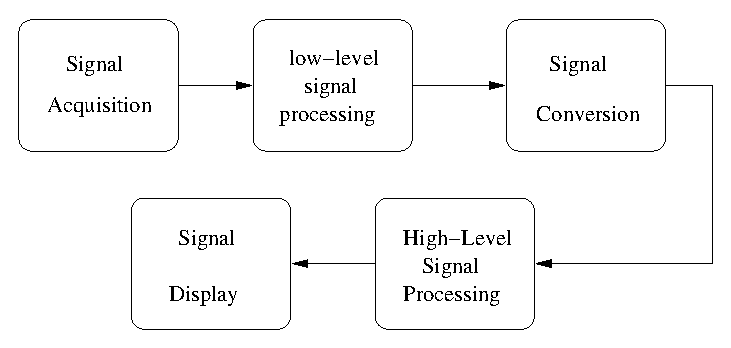
\includegraphics[width=\textwidth]{./overview.eps} 
        \caption{System overview.}
        \label{fig:overview}
\end{figure}

Figure ~\vref{fig:overview} depicts the system as a logical and
physically separated set of five independent functional modules. Each
module is named according to its primary function:

\begin{itemize}
	\item{ A signal acquisition model containing a set of active
		  electrodes mounted on a adjustable head--band. This module
		  sets the system apart from more traditional EEG data
		  acquisition systems. [Chapter~\ref{chap:sa}].}
	\item{ A low--level signal processing module responsible for the
		  extraction and amplification of the EEG signal from the
		  acquired scalp signal. This module is implemented using
		  standard differential instrumentation amplifiers
		  [Chapter~\ref{chap:llsp}].}
	\item{ A signal conversion module used to digitize the extracted
          EEG signal [Chapter~\ref{chap:sc}].} This module is
		  implemented using of--the--shelf hardware and software.
	\item{ A high level signal processing module that allows for
	      specialized spectral processing and feature extraction
	      sub-modules [Chapter~\ref{chap:hlsp}].} This module is
		  implemented using commercial software. 
	\item{ A signal display module capable of displaying both the raw
		  EEG signal from the signal conversion module and the results
		  generated by the high--level signal processing module
		  [Chapter~\ref{chap:hlsp}].} This module is implemented using
		  standard PC hardware and commercial software.
\end{itemize}
	

Each module is designed and implemented with the reduction of
environmental and system noise as primary goal. Various techniques are
employed to prevent the degradation of the EEG signal by both external
interference and internal noise sources within each system module.


\section{General Specification}
\label{section:def-of-need}

Developing a set of definitive goals from a general specification
naturally leads toward and ultimately translates into a quantitative
system specification. Translating fuzzy concepts of
``user--friendliness'', ``ease--of--use'' and ``adequate signal
quality'' to measurable constants sets a qualitative standard against
which real progress and eventual system compliance may be evaluated.

\subsection{Terms and definitions}
\subsubsection{User--friendliness and ease of use}
User--friendliness and ease of use are qualitative ergonomic
specifications implying that the operator be allowed to achieve her
purpose with the minimum amount of system imposed constraints. This
includes among other things mobility constraints due to signal and
power cable lengths. The following quantitative values were chosen to
define ease of use and user--friendliness:

\begin{itemize}
	\item{Application and adjustment time: The maximum time spent to
	physically attach the active--electrode array - 10~s.}
	\item{Removal time: The maximum time spent removing the
	active--electrode array 5~s.}
	\item{Preparation time: Time spent to prepare the skin surface for
	the application of electrodes - none}
	\item{User discomfort: User discomfort is quantified as a function of
	the headband's weight and skin contact area. Acceptable values
	are: Weight 400~g, Contact Area 10~$cm^{2}$}
\end{itemize}

\subsubsection{Adequate signal quality.}
System signal quality is the underlying basis for the technical design
specification of the system and is the ultimate factor determining the
overall usability of the system. Signal quality is measured in terms
of the signal to noise ratio at the output of the signal conversion
module. The signal to noise ratio is defined throughout this document
as 20log10$(\frac{V_{s}}{V_{n}})$ with $V_{s}$ the EEG signal voltage
and $V_{n}$ the sum of all system and environmental noise
voltages. The minimum acceptable $S/N$ value is specified as
20~dB. The signal voltage must have a amplitude at least ten times the
noise voltage.

Table ~\vref{table:hl-design-contraints} summarizes the general
high-level system specification. 

\begin{table}
\begin{center}
\caption{High--level design constraints}
\label{table:hl-design-contraints}	
\begin{tabular}{|l|l|} 	\hline	
	Application and adjustment time & 10.0~s\\
	Removal time & 5~s\\
	Preparation time & 0~s\\
	Head--band Weight & 200~g\\
	Contact Area & 10~cm$^{2}$\\
	Signal conversion output minimum S/N & 20~dB \\\hline
\end{tabular}
\end{center}
\end{table}



\section{High level system specification}
\label{section:hl-system-specification}
In order to satisfy the conditions specified in the definition of need
(Section~\vref{section:def-of-need}) a top-down system design approach
is adopted leading to a modular system design. Modularizing the system
eases the testing and evaluation process significantly and allows the
design to budget for acceptable noise levels within the individual
modules. As noise added to the system by a module is cascaded into the
next module as part of the input signal it imperative that module
level noise sources be suppressed as far as possible. Adequate
screening is applied to limit the effect of environmental signal
contamination. Noise introduced by the environment will hence forward
be referred to as interference.


The system consists of several modules or sub--systems. The design
accommodates the whole measurement process in a modular environment
which is closely integrated but easily customizable to suit the needs
of a particular measurement. Each module in the system object diagram
is implemented and tested in isolation before being integrated with
the rest of the system. This process contributed to the need of a
standard test or measurement environment. The Standard measurement
environment (SME) is discussed in Chapter~\ref{chap:sme}.

\begin{figure}[htbp]
\begin{center}
        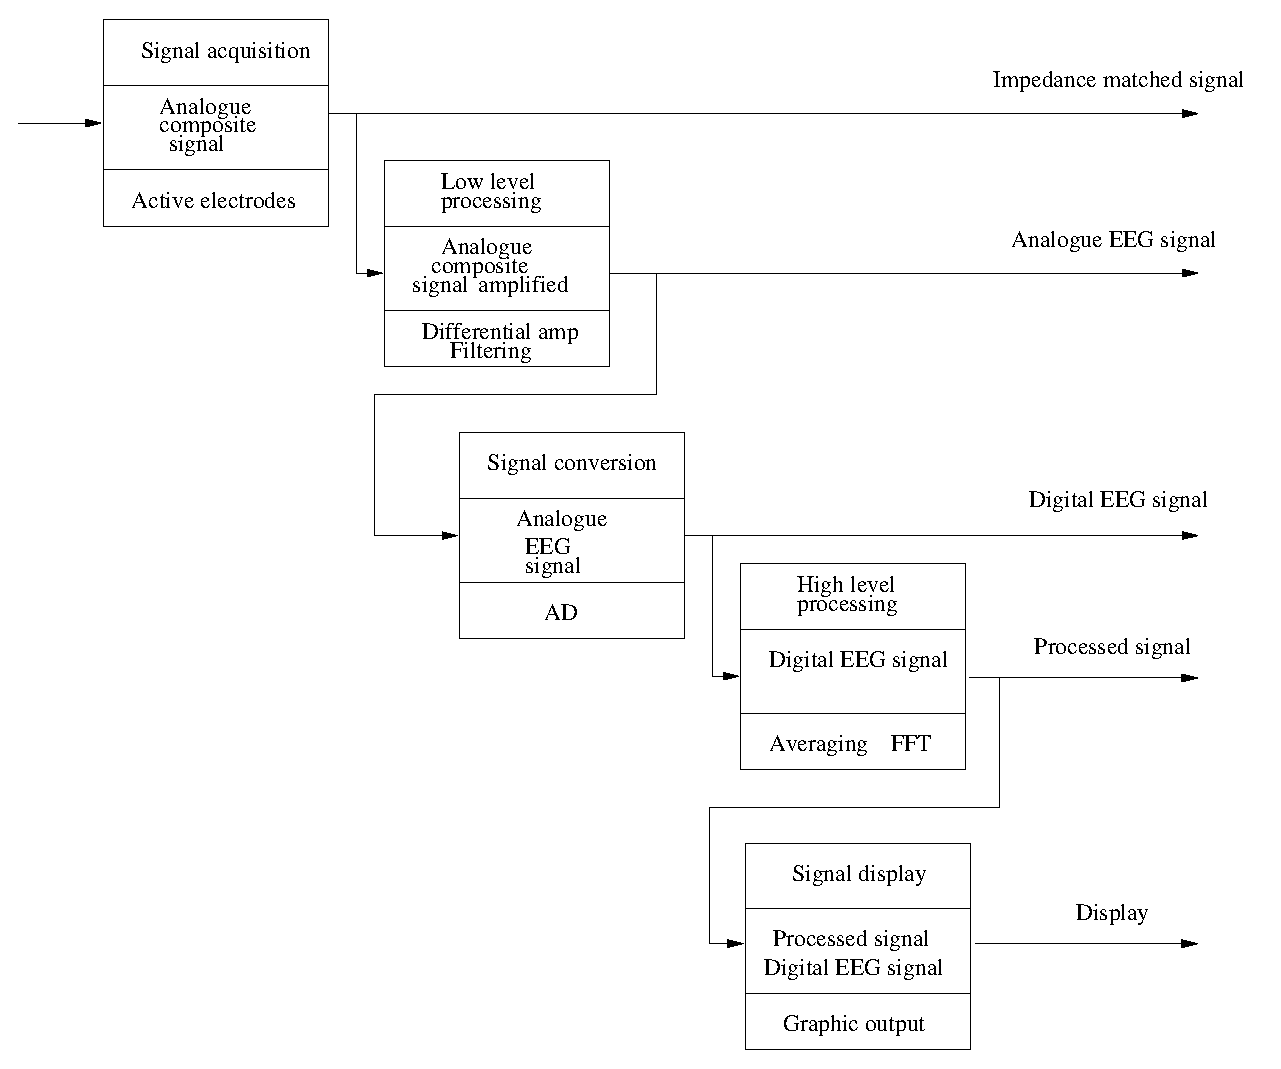
\includegraphics[width=\textwidth]{eeg-signal-flow.eps}
        \caption{System signal flow diagram.}
        \label{fig:eeg-signal-flow}
\end{center}
\end{figure}

The system signal flow diagram depicted in
Figure~\vref{fig:eeg-signal-flow} illustrates the flow of the EEG
signal through the system. The signal enters the system at the signal
acquisition module, moves through the various modules and ends up in
the signal display module.

The system consists of five distinct modules:

\begin{itemize}
	\item{Signal acquisition module. }
	\item{Low level signal processing module.}
	\item{Signal conversion module.}
	\item{High level signal processing module.} 
	\item{Signal display module.}
\end{itemize}

A brief description of each module follows. Each module has a chapter
dedicated to it and is discussed at length therein.


The \textbf{signal acquisition module} (SAM) acquires the EEG signal
from the scalp. The SAM module is the system's primary physical
interface with the user. The implementation of this module have to
comply to the prerequisites of weight and contact area specified in
the definition of need. This module makes use of a FET-driven
active--electrode array which reduces the severity many of the
problems associated with traditional electrodes. The electrode array
is implemented using low noise FET--input operation amplifiers. The
array is mounted on a user--adjustable head--band. The user may set
the pressure exerted by the metal conductors on the scalp to a
comfortable level by adjusting the head--band appropriately.


The \textbf{low--level signal processing module} (LLSPM) extracts,
amplifies and filters the EEG signal from the SAM output signal. The
LLSPM is a critical system module and is designed and implemented with
cognizance of noise contamination from external as well as internal
sources. Signal contamination concerns ensures that care is taken to
screen this module adequately. A shoddy implementation of a sound
design will render the system useless. Monolithic differential
amplifiers are used in this module as well as switched capacitor
filters. 


The \textbf{signal conversion module} (SCM) digitizes the analogue EEG
signal for further processing by the secondary signal processing
module. This module consists of a commercial analogue to digital (A/D)
system. Signal noise introduced by the conversion process is
considered to some degree in the SCM's design.

The \textbf{high level signal processing module} (HLSPM) is
responsible for complex signal manipulation. This includes averaging
and feature extraction modes. Real time as well as off--line
processing is possible. 


The \textbf{signal display module} (SDM) displays the results produced
by the HLSPM. This module is closely associated with the high level
signal processing module, the HLSPM is however not bounded to any
specific graphical interface. In compliance with the basic UNIX
philosophy of modularizing software the HLSPM and SDM are separate
packages. This enables a Internet--connected investigator to monitor
running experiments from any Internet access point. This module is
also implemented using custom made Linux based software and available
libraries.


\section{The standard measurement environment}
In order to test the various modules during the different stages of
system development and the system as a whole, a standard measurement
environment (SME) was developed and used. The SME consists of a
physical and electrical model of the human head and emulates the
signal conditions present at the scalp. The use of a standard
measurement environment makes the quantitative evaluation of a
module's performance with different configurations possible. The SME
is applied as a test bench and a rapid development tool throughout
the system design cycle.


\section{Report structure}
The design and implementation of each module is discussed in this
report. The general structure of this document follows the general
signal path of the EEG signal, as depicted in the signal flow diagram
of Figure~\vref{fig:eeg-signal-flow}. The design and implementation of
the standard measurement environment is discussed first as all other
modules were tested and developed using the standard measurement
environment.


The design specifications and implementation detail for a module is
discussed under that module's name as described in
Figure~\vref{fig:eeg-signal-flow} and
Section~\ref{section:hl-system-specification}. Secondary
considerations concerning the design and implementation of a specific
module are also included in the discussion when necessary. Appendices
are used when the subject matter warrants it.


























\chapter{The Standard Measurement Environment} \label{chap:sme}
%sme.tex
%included in skripsie.tex

\section{Overview}
In order to test the individual system modules as well as the complete
system during its different development stages a standard measurement
environment (SME) was developed and used.The SME consists of a
physical and electrical model of the human head and emulates the
signal conditions present on the scalp surface. The use of a standard
measurement environment makes the quantitative evaluation of a
module's performance with different configurations possible. The SME
is applied as a test bench and a rapid development tool throughout the
system design cycle.


The decision to use a standard measurement environment was made in
part to circumvent logistical and safety constraints encountered while
testing system modules with human subjects:

\begin{itemize}
	\item{Protecting the subject from macro-shock conditions
	unnecessarily complicates the test procedure and system under
	investigation without any real benefit to the investigative
	process.}

	\item{The skin impedance of the subject is a function of room
	temperature and humidity. These variables may change while testing
	is in progress, obscuring parameters under observation. The
	electrode half--cell potential varies with skin pH levels and
	between electrode applications. Environmental conditions must be
	controlled to keep skin characteristics constant, complicating the
	process of system evaluation.}

	\item{The emotional condition of the subject, degree of brain
	activity, levels of stress and specifically ocular artifacts can
	complicate the testing procedure in masking unwanted internal
	noise sources with unrelated physiological signals.}
	\item{The skin potential between the stratum corneum and the
	stratum germinativum varies between individuals and is easily
	modulated by environmental conditions. This complicates the
	verification and comparison process to a large degree.}
\end{itemize}

Eliminating the need for a human signal source eases the system
development cycle and simplifies the process of evaluating the
variance of a single system parameter during a test run. 

The SME simplifies the process of testing different module
configurations while keeping external system variables constant. Using
a standard measurement environment makes it possible to vary specific
model parameters while keeping others constant. 

\section{SME design specification} \label{section:sme-design-spec}

\begin{figure}[htbp]
\begin{center}
		\psfrag{delta}{$\delta$}			
		\psfrag{theta}{$\theta$}			
		\psfrag{alpha}{$\alpha$}			
		\psfrag{beta}{$\beta$}			
		\psfrag{gamma}{$\gamma$}			
		\psfrag{Vrms}{$\mu\/V_{RMS}$}			
        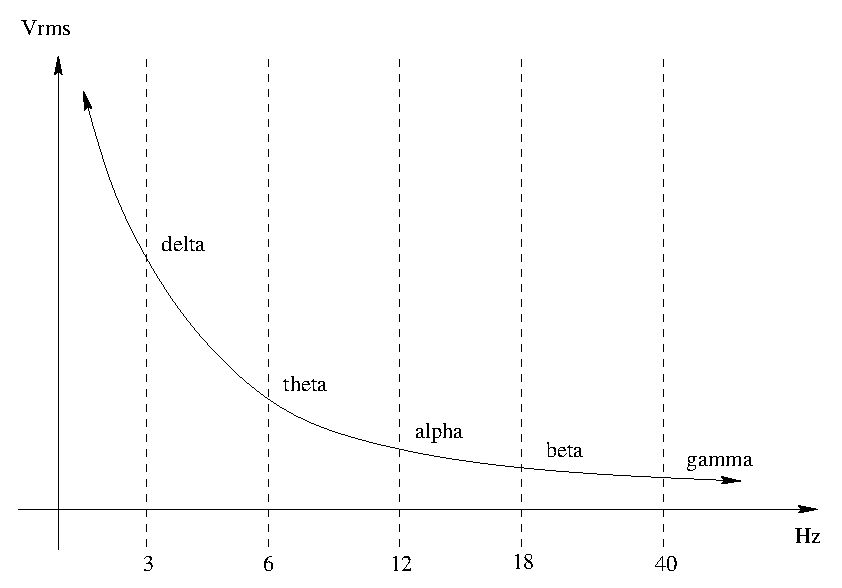
\includegraphics[width=\textwidth]{sme-eeg-power.eps}
        \caption{Simulated EEG power distribution}
        \label{fig:sme-eeg-power}
\end{center}
\end{figure}


To replace the need for a human subject the SME must be able to
accurately emulate the electrical conditions encountered on the
surface of the human scalp. Figure~\vref{fig:sme-eeg-power} depicts a
idealized EEG power spectrum as measured from various montage points
on the scalp surface. The SME's high level design specification simply
states that the SME must be able to generate a output signal having
the same power and frequency characteristics depicted in
Figure~\vref{fig:sme-eeg-power} when measured with a differential
amplifier under normal conditions. Normal conditions imply that the
amplifier has to cope with a input signal with a minimum common mode
component of 80~dB above the differential signal level.


In short: The SME must provide a output signal composed of a source
signal in the 0.1~Hz to 35~Hz band on which a +80~dB common mode
signal is superimposed. The RMS signal power levels must be within
50\% of the Figure~\ref{fig:sme-eeg-power} specification. 

In order to simplify the SME implementation and the individual
module's testing procedures only five discrete frequencies are used
for testing.

\begin{figure}[htbp]
\begin{center}
	\psfrag{eeg}[][]{$e_{EEG}$}
	\psfrag{nv}[][]{$[\mu\/V_n]$}
	\psfrag{t}[][]{time [s]}												
	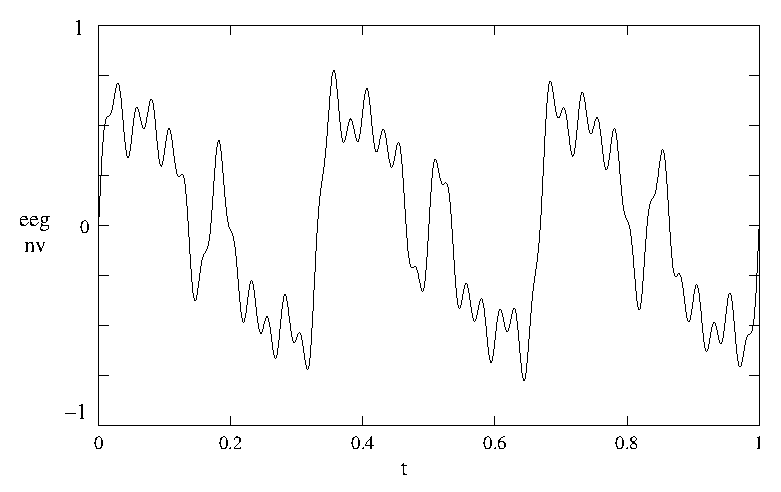
\includegraphics[width=\textwidth]{time-sim.eps}
    \caption{Simulated EEG signal.}
    \label{fig:time-sim}
\end{center}
\end{figure}

\begin{equation} \label{eq:time-sim}
	e_{EEG}(t) = \sum_{n=1}^5 A_{n}sin(f_{n}t2\pi)
\end{equation}

With $A_n$ the amplitude of the sinusoidal component $n$ and $f_n$ the
frequency of sinusoidal signal component $n$. The values of $A_n$ and
$f_n$ are listed in Table~\vref{table:test-pros}.


Figure~\vref{fig:time-sim} depicts a normalized simulated EEG signal
$e_{EEG}$ consisting of only the five frequency components noted in
Figure~\vref{fig:sme-eeg-power}. The composite signal of
Figure~\ref{fig:time-sim} is not a accurate representation of the
simulated cranial signal used during SME tests. A single frequency is
normally used for testing. Generating composite signals unnecessarily
complicates the implementation of the SME with no comparative added
functionality. The simulated signal of Figure~\vref{fig:time-sim} can
be generated by summing the outputs of the signal generators. 

Table~\vref{table:test-pros} is used during system and system module
evaluation. The $V_{pp}$ values specified is representative of the
power distribution graph depicted in Figure~\ref{fig:sme-eeg-power}.


\begin{table}
\begin{center}	
	\begin{tabular}[htpb]{|c|c|c|c|} \hline
	No. & Mark & Frequency [Hz]  & $V_{pp}$  \\ \hline
	1 & $\delta$ & 3 & 100~$\mu\/V$ \\
	2 & $\theta$ & 6 & 100~$\mu\/V$ \\
	3 & $\alpha$ & 12 & 10~$\mu\/V$ \\
	4 & $\beta$ & 18 & 20~$\mu\/V$ \\
	5 & $\gamma$ & 40 & 2~$\mu\/V$ \\
	\hline
	\end{tabular}
	\caption{SME output signal quantitative specification}
	\label{table:test-pros}
\end{center}	
\end{table}

\section{SME design and implementation}
The SME consists of a physical and electrical model of the human
head. The physical module aids in achieving the ergonomic design goals
set in section~\vref{section:def-of-need}. The physical model also
serves as a test bed for evaluating variations in the signal
acquisition module's container design. A electrical model is
implemented using sinusoidal and noise signal generators. The SME
presents a model signal to the signal acquisition module incorporating
the main characteristics of a natural cranial surface signal.

\subsection{SME Physical model}

\begin{figure}[htbp]
\begin{center}
	\psfrag{Base strips}[][]{Base strips}
	\psfrag{Head model}[][]{Head Model}
	\psfrag{Electrode contacts}{Electrode contacts}	
	\psfrag{Common mode }[][]{Common mode}							
	\psfrag{and signal}[][]{and signal }
	\psfrag{source}[][]{source}
	\psfrag{EM shielding}[][]{EM Shielding}
	\psfrag{SA }{SA }
	\psfrag{Module}{Module }
	\psfrag{Container}[][]{Container}
	\psfrag{fp1}[][]{$F_{p1}$}				
	\psfrag{fp2}[][]{$F_{p2}$}
	\psfrag{ref}[][]{$ref$}	
	\psfrag{ec}[][]{ ($e_c$)}		
	\psfrag{eb}[][]{ ($e_b$)}												
    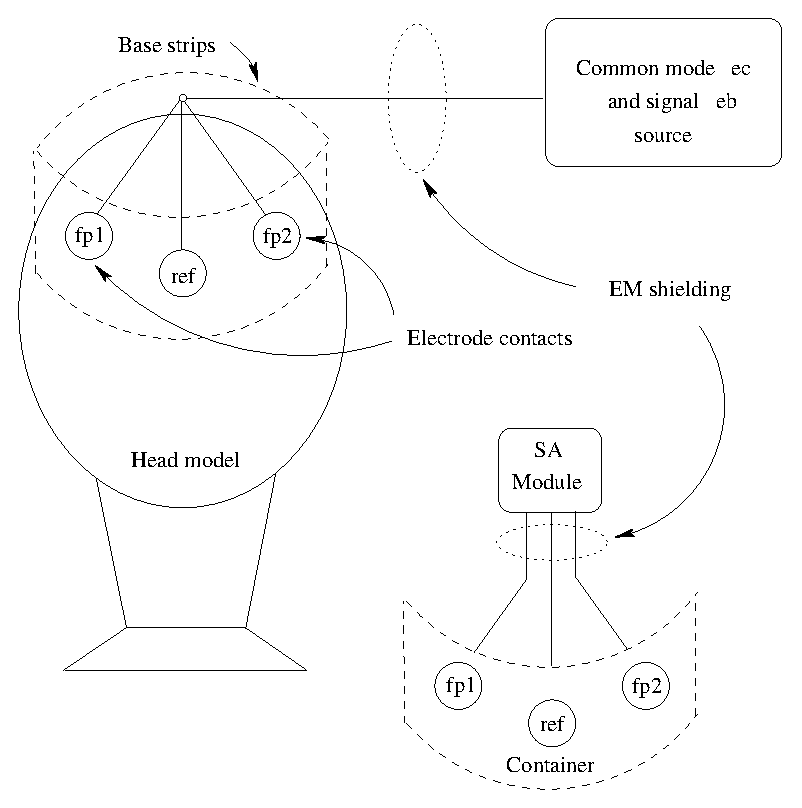
\includegraphics[width=\textwidth]{standard-measurement-environment.eps}
    \caption{Physical model of the standard measurement environment.}
    \label{fig:standard-measurement-environment}
\end{center}
\end{figure}


Figure~\vref{fig:standard-measurement-environment} is a diagram of the
physical model of the SME. The SME module is constructed using a
standard polystyrene hat--fitter head model. These models are widely
available and easily replaceable. The polystyrene model is painted to
provide a extra protective layer against the wear and tear of
laboratory use.  Horizontal and vertical foam rubber strips are glued
onto the painted surface to assist in the physical fitting of the
container. Electrical contacts are fastened to the surface rubber
strips at the $F_{p1}$ and $F_{p2}$ locations as defined by the 10--20
EEG montage protocol
\cite[p3-4]{eeghand}. Accurately establishing the physical distance
between the electrodes on the SME ensures that the signal acquisition
module (SAM) takes the possible detrimental effect of interference
from lead wires into account. The electrode contacts are connected to
the signal generators $e_b$ and $e_c$
(Figure~\ref{fig:standard-measurement-environment}) via 5~cm lengths
of shielded wiring. The signal generators are mounted close to the
electrical contacts on the rear side of the head model, see
Figure~\vref{fig:sme-photo}.


The removable SAM--container is mounted on top of the base strip with
the electrodes touching the electrical contacts. This arrangement
enables the worker to easily test and calibrate the various modules
and the complete system, while keeping the physical and electrical
model parameters constant. The container hosts the signal acquisition
module electronics and does not logically fit with the SME. The
container is depicted with
Figure~\ref{fig:standard-measurement-environment} to illustrate the
physical fit between the SME and the signal acquisition module while
testing the various system modules.

\begin{figure}[htbp]
\begin{center}
	%\vspace{8cm}
	\includegraphics*{sme-head.eps2}
	\caption{SME Photograph}
\label{fig:sme-photo}
\end{center}
\end{figure}

Figure~\ref{fig:sme-photo} is a photograph of the SME module used
during testing and development. The electrical contacts can be seen at
the $F_{p1}$ and $F_{p2}$ positions. The signal generators are
mounted to the rear of the model below the inion. The Signal
Acquisition module's container is fastened on top of the the SME with
the electrodes aligned over the electrical contacts using Velcro
strips.



\subsection{SME Electrical model}
\begin{figure}[ht]
\begin{center}
	\psfrag{Head}{Head}
	\psfrag{A}{A}
	\psfrag{B}{B}
	\psfrag{re}{$r_e$}		
	\psfrag{rc}{$r_c$}		
	\psfrag{eb}[][]{$e_b$}		
	\psfrag{ec}[][]{$e_c$} %common signal across dif inputs 		
	\psfrag{Eeeg}[][]{\colorbox{white}{$e_{EEG}$}}			
	\psfrag{r1}{$R_{s1}$}
	\psfrag{r2}{$R_{s2}$}				
	\psfrag{c1}{$C_1$}		
	\psfrag{c2}{$C_2$}		
	\psfrag{O1}{$O_1$}		
	\psfrag{O2}{$O_2$}		
	\psfrag{O3}{$ref$}		
	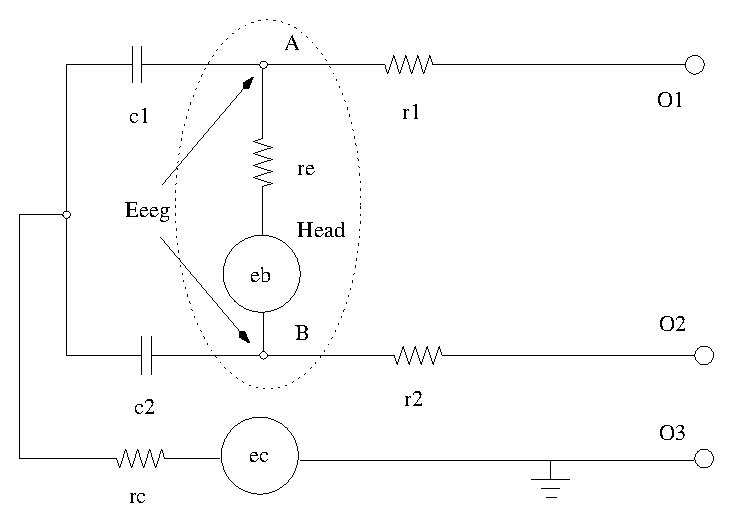
\includegraphics[width=\textwidth]{sme-eq.eps}
	\caption{Electrical model of the standard measurement environment.}
	\label{fig:sme-eq}
	\end{center}
\end{figure}

The SME must be able to emulate the electrical behavior normally
measured on the scalp surface for experimental and modeling
purposes. The brain is the source of the electrical activity measured
as the EEG signal. The dry skin surface as well as the underlying soft
tissue acts as volume conductors from the signal source to the
electrode surfaces. The conduction pathways tend to act as low--pass
signal filters attenuating the signal. This behavior is simulated with
a resistive circuit that lumps the various skin impedances together.

Figure~\vref{fig:sme-eq} summarizes the electrical model implemented
by the SME.
\begin{itemize}

	\item{Outputs $O_1$ and $O_2$ represent the SME output
	signals. The $ref$ label represents the SME signal ground
	reference. The output signals and signal ground are accessible
	through electrical contacts mounted on the SME physical model, see
	Figure~\vref{fig:standard-measurement-environment}.}


	\item{The $R_{s1}$ and $R_{22}$ values are the equivalent scalp
	resistances. $R_{s1} = R_{s2} = 10~k\Omega$
	\cite{intro-to-bio}.}

	\item{The $e_b$ signal is the Th\`{e}venin equivalent voltage
	source as seen by the electrodes (A-B). The $e_b$ voltage is the
	representation of all electrical activity volume conducted to a
	central point between electrodes. This signal is chosen from the
	options available in Table~\ref{table:test-pros} depending on
	module being developed or tested. The 12~Hz $\alpha$ signal were
	used most frequently as it lies fairly central in the EEG band of
	interest.}

	\item{The $r_e$ value is the Th\`{e}venin equivalent resistance of
	the signal source as seen by the electrodes (A-B). The $r_e$ value
	was chosen as 10~k$\Omega$, \cite{intro-to-bio}.}

	\item{Common source signal $e_c$ is capacitively coupled through
	$C_1$ and $C_2$ into $O_1$ and $O_2$. The common-mode voltage
	$e_c$ simulates all interference signal sources attributable to
	50~Hz power--line noise, power equipment and fluorescent lights
	\cite{fluorescent-interference},
	\cite{fluorescent-interference2}. The values of $C_1$ and $C_2$
	was chosen as 2pF, \cite{drive}, and $r_e = 10~k\Omega$.}
\end{itemize}

The EEG signal $e_{EEG}$ is generated using a approximately 100~$\mu$V
sinusoidal signal source. Common mode voltage $e_c$ is the sum of two
large amplitude signals, a sinusoidal signal $e_{cs}$ (1--100~mV) and
a white noise signal $e_{white}$ with amplitude range
1~mV$_{rms}$--100~mV$_{rms}$. The white noise signal ($e_{white}$) is
used during bandwidth tests and can be coupled in and out of the
SME. The common mode voltage $e_c$ is added to $e_{EEG}$ via $C_1$ and
$C_2$. A differential measurement between $O_1$ and $O_2$ with respect
to $ref$ yields a signal similar to $e_{EEG}$.

Although this model of electrical scalp activity is rather contrived
it adequately serves the purpose for which it was designed.

\subsubsection{Interference reduction}
In order to eliminate external interference the complete SME
environment is housed in a rectangular 100X150X50~cm metal box acting
as a Faraday cage. The cage is manufactured from plate metal and
square tubing. The cage interior is accessed via a hinged hatch,
forming one of the cage walls when shut.

The SME is electrically accessed via a set of 2~mm female RCA jacks
and is internally powered from a set of re-chargeable 9~V
nickel--cadmium batteries. Electrically isolating the whole SME
environment allows for the rapid prototyping of system modules without
the added complexity of uncontrolled signal contamination due to
external interference.

The rest of this chapter is dedicated to the implementation details of
the signal generators used in generating $e_c$ and $e_{EEG}$.


\subsection{Signal generation overview}
\label{section:sin}
Two distinct signal types are used in the SME -- sinusoidal signals
and white noise. The generators used to create $e_{EEG}$ and the
sinusoidal component of $e_c$ differ only in the signal output
amplitude and frequency. The same basic circuit is used to implement
all sinusoidal signal generators in the SME. The common mode signal
$e_c$ has a white noise component $c_{white}$ used during noise
suppression and filter bandwidth tests. The $c_{white}$ circuit is
implemented using a zener diode as noise source.


The common mode signal $e_c$ is the sum of a sinusoidal ($e_{cs}$) and
a white noise ($e_{white}$) signal. Separate signal generators are
used to create the $e_{white}$ and $e_{cs}$ components of $e_c$. The
common mode signal is summed with $e_{EEG}$ via the couple
capacitances $C_1$ and $C_2$ of Figure~\ref{fig:sme-eq}. The
amplitude and bandwidth variable common mode signal source is used to
evaluate a module's dynamic response as well as the common mode
rejection ratio of the low level signal processing module.


The various filters used throughout the system is tested by adjusting
the frequency of $e_c$ beyond the evaluated filter's cut--off point,
and measuring the resulting output signal. Because EEG signals,
external interference and internal system generated noise are all
inherently stochastic by nature this approach is considered to be a
good emulation of normal system behavior.

\subsection{Sinusoidal signal generation - $e_b$ and $e_{cs}$} 
\label{section:wein}
\subsubsection{Overview}
The SME electrical model makes use of sinusoidal signal generators as
both common--mode ($e_c$) and differential--mode ($e_b$) signal
sources. A common Wein--bridge circuit design \cite[p30-32]{analog}
\cite[p344-349]{master} \cite[p296-297]{art} 
is used in implementing all the sinusoidal signal generators used in
the SME. The specific component values are varied to achieve desired
frequency and amplitude specifications.

\subsubsection{Design specification}
The sinusoidal signal generators used in the SME are required to be
exceptionally pure and stable. A test signal must have a internal
distortion factor at least ten times smaller than the expected system
distortion levels to establish a accurate representation of the system
distortion, \cite[p296]{art}. A stable oscillator design with maximum
residual distortion of less than 0.05\% is called for.

\subsubsection{Implementation}
\begin{figure}[htbp]
\begin{center}
	\psfrag{+}{+}
	\psfrag{-}{--}
	\psfrag{a}{$a$}
	\psfrag{b}{$b$}
	\psfrag{r}{$R$}
	\psfrag{c}{$C$}
	\psfrag{rf}{$R_{fb}$}
	\psfrag{ira}{$i_{R_{ad}}$}
	\psfrag{ra}{$R_{ad}$}
	\psfrag{vsin}{$e_{sin}$}
	\psfrag{TL071}[][]{071}
	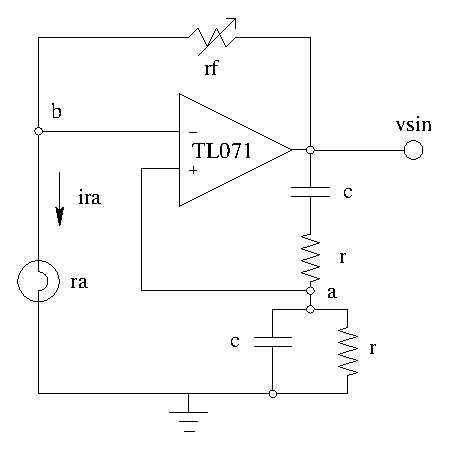
\includegraphics{sin-source.eps}
    \caption{Sinusoidal signal generator.}
    \label{fig:sin-source}
\end{center}
\end{figure}

Wein--bridge oscillators are known for their exceptional stability and
low distortion at low frequencies. The signal generator of
Figure~\ref{fig:sin-source} consists of an operational amplifier with
two complex impedances in its positive feedback path forming one tier
of the bridge. The circuit operates in non-inverting mode with the
non-inverting input signal $v_a$ created by the voltage divider at
node $a$. The negative feedback path consists of two real impedances
controlling circuit gain. $R_{ad}$ is a filament lamp with resistance
inversely proportionate to current.



\subsubsection{Circuit analysis}
The circuit analysis of the circuit in Figure~\vref{fig:sin-source} is
done by equating the real and imaginary components of $v_a$ and $v_b$,
\cite[p31]{analog}.

The impedance of the series $RC$ network is:
\begin{equation}
	Z_{s} = \frac{1 + sRC}{sC}
	\label{eq:zs}
\end{equation}

The impedance of the parallel $RC$ network is:
\begin{equation}
	Z_{p} = \frac{R}{1 + sRC}
	\label{eq:zp}
\end{equation}

At node $a$, the non-inverting amplifier input, the voltage $v_a$ is
determined by the voltage divider formed by $Z_{s}$ and $Z_{p}$:
\begin{equation}
	v_{a} = \frac{e_{sin}RCs}{R^2C^2s^2 + 3RCs + 1}
	\label{eq:va}
\end{equation}

At node $b$, the inverting amplifier input, the voltage $v_b$ is
determined by the voltage divider formed by $R_{fb}$ and $R_{ad}$:
\begin{equation}
	v_{b} = \frac{e_{sin}}{1 + \frac{R_{fb}}{R_{ad}}}
	\label{eq:vb}
\end{equation}

The operational amplifier adjusts $e_{sin}$ to equate $v_a$ and $v_b$
via the positive and negative feedback loops, from the amplifier
action follows that:
\begin{equation}
	\frac{RCs}{R^2C^2s^2 + 3RCs + 1} = \frac{1}{1 + \frac{R_{fb}}{R_{ad}}}
	\label{eq:va=vb}
\end{equation}

For a constant $e_{sin}$ output amplitude $\sigma$ is set to zero in
$s = \sigma +j\omega$.  Substituting $s = j\omega$ in
Equation~\ref{eq:va=vb} and grouping real and imaginary terms yields
Equation~\ref{eq:va=vb} in terms of $\omega$:
\begin{equation}
	\frac{-\omega\/RC}{j(1 - \omega^2R^2C^2) - 3\omega\/RC} =
	\frac{1}{1 + \frac{R_{fb}}{R_{ad}}} 
	\label{eq:va=vbj}
\end{equation}

Equating imaginary terms on both sides of Equation~\ref{eq:va=vbj}
yields the equation for calculating the frequency of the output signal
$e_{sin}$.
\begin{equation}
	1 - \omega\/^2R^2C^2 = 0
	\rightarrow f = \frac{1}{2\pi\/RC}
	\label{eq:f}
\end{equation}

Equating real terms on both sides of Equation~\ref{eq:va=vbj} yields
the relationship between $R_{fb}$ and $R_{ad}$:
\begin{equation}
	R_{fb} = 2R_{ad}
	\label{eq:r}
\end{equation}

Substituting $R_{fb} = 2R_{ad}$ in Equation~\ref{eq:vb} and solving
for $\frac{e_{sin}}{v_b}$ yields a circuit gain $G = 3$. $R_{ad}$
varies with the current ($i_{R_{ad}}$)flowing through it stabilizing
the system gain. If $G < 3$ more energy is lost than being added and
oscillations die out, if $G > 3$ the amplifier saturates and $e_{sin}$
converges to one of the supply rail voltages. The feedback resistance
$R_{fb}$ is adjusted to 2$R_{ad}$, when $e_{sin}$ decreases the
$i_{R_{ad}}$ current through $R_{ad}$ decreases causing $R_{ad}$'s
temperature to drop. A decrease in $R_{ad}$ temperature lowers its
resistance which causes the circuit gain and consequently $e_{sin}$ to
increase proportionately. This cyclic behavior is governed by the
large time constant gain setting feedback introduced by $R_{ad}$.

Using Equations~\ref{eq:f} and \ref{eq:r} circuit component values can
be computed to satisfy the requirements of each sinusoidal signal
generator needed in the SME.

\begin{figure}[htbp]
	\begin{center}
	\psfrag{r}{$R$}
	\psfrag{f}{$f$}
	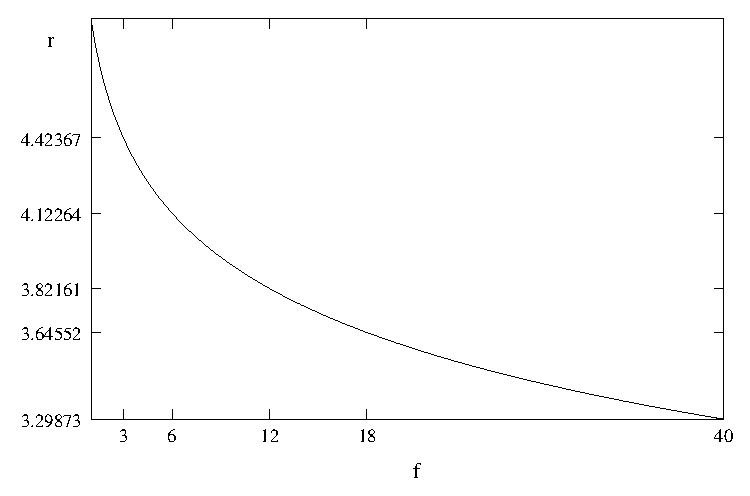
\includegraphics[width=\textwidth]{sin-r.eps}
    \caption{Resistance--Frequency (C=2~$\mu$F)}
    \label{fig:sin-r}
	\end{center}
\end{figure}

Figure~\vref{fig:sin-r} plots $R = log_{10}(\frac{1}{2\pi\/RC})$ for a
chosen capacitance $C = 2\mu$F. From Figure~\vref{fig:sin-r}
approximate resistance values are chosen, these are listed in
Table~\vref{table:r-c}. The precision of the quoted values does not
reflect the accuracy of the resistances used in the generator
implementation. Although 1\% resistances were used throughout the
design, values can only be chosen from a fixed set. Where appropriate
resistances were corrected using series or parallel combinations.


\begin{table}
\begin{center}	
	\begin{tabular}[htpb]{|c|c|l|l|} \hline
	No. & Mark & Frequency [Hz]  & $R$  \\ \hline
	1 & $\delta$ & 3 & 26.5~k$\Omega$ \\
	2 & $\theta$ & 6 & 13.3~k$\Omega$ \\
	3 & $\alpha$ & 12 & 6.7~k$\Omega$ \\
	4 & $\beta$ & 18 & 4.4~k$\Omega$ \\
	5 & $\gamma$ & 40 & 2.0~k$\Omega$ \\
	\hline
	\end{tabular}
	\caption{Resistance values for $C=2~\mu\/F$}
	\label{table:r-c}
\end{center}	
\end{table}

All resistances are 1\% accurate metal--film devices with good
temperature stability. Polypropylene capacitors are used because of
their good accuracy, temperature stability and low leakage properties,
\cite[p22]{art}.


\subsection{Noise generation - $e_{white}$}
\label{section:noise}
\subsubsection{Overview}
This section details the design and implementation of the noise
generator used in the standard measurement environment. The noise
source $e_{white}$ is applied capacitively to both electrodes and is a
component of the common--mode signal as seen by the differential
inputs of the low level signal processing module.


\subsubsection{Design specification}
The noise generator must be capable of generating a relatively flat
spectrum white noise signal in the 0.1~Hz to 200~Hz range. White noise
is defined as having equal power per Hz, the noise generator only
needs to approximate a white noise source in the operative bandwidth.


\subsubsection{Implementation}
The noise generator is implemented using analog electronic circuitry
based on the avalanche noise generated by a reverse biased zener
diode. Avalanche noise is created when a PN junction is operated in
reverse breakdown mode \cite[p3]{noise-analysis}. Electrons accelerate
in the reverse electric field within the PN junction depletion zone
gathering enough kinetic energy to dislodge other electrons from the
atoms in the junction crystal lattice.

Good quality low--voltage zener diodes are not readily available
commercially and an alternative device is used instead.

The LM336 device simulates a low voltage zener diode and is ideally
suited for analogue noise generator applications. The low device
voltage supports long battery life in operation. The LM336 may be
operated over a wide voltage range which further extends the usable
battery life. The device noise specification is available from the
product specification sheet. The frequency response noted in the
product sheet is a valuable yardstick when evaluating the individual
module frequency responses. The frequency response of each module is
compared with the LM336 product sheet noise specification and must
correlate to a high degree for an adequately designed and implemented
module.

\begin{figure}[htbp]
	\begin{center}
	\psfrag{1}{1}
	\psfrag{2}{2}
	\psfrag{3}{3}
	\psfrag{8}{8}
	\psfrag{r1}{$R_1$}
	\psfrag{r2}{$R_2$}
	\psfrag{r3}{$R_3$}
	\psfrag{c1}[][]{\colorbox{white}{$C_1$}}	
	\psfrag{c2}[][]{\colorbox{white}{$C_2$}}	
	\psfrag{c3}{$C_3$}
	\psfrag{c4}{$C_4$}
	\psfrag{c5}[][]{$C_5$}
	\psfrag{c6}{$C_6$}
	\psfrag{c7}{$C_7$}
	\psfrag{ew}{$e_{white}$}
	\psfrag{+}{+}		
	\psfrag{-}{--}
	\psfrag{+9V}{+9 V}
	\psfrag{LM336}[][]{LM336}				
	\psfrag{386}[][]{386}				
	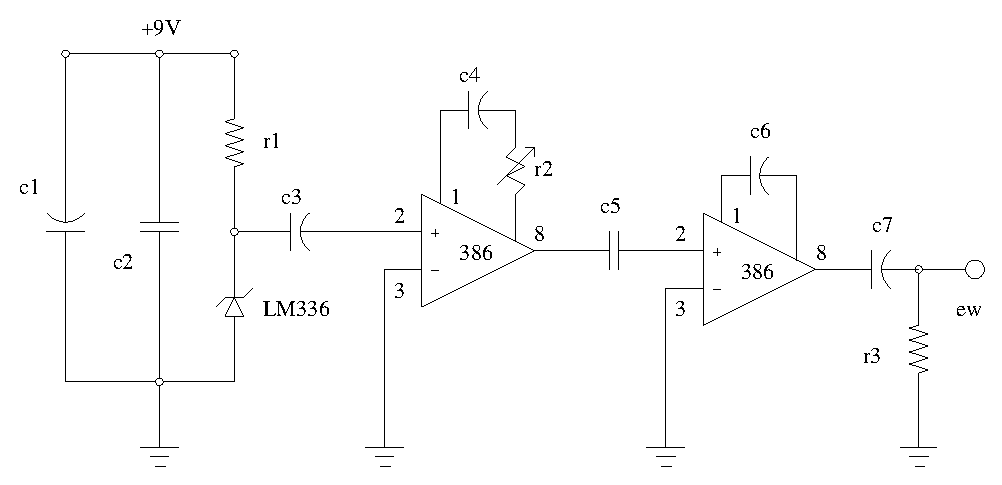
\includegraphics[width=\textwidth]{noise-generator.eps}
    \caption{White noise generator.}
    \label{fig:noise-generator}
	\end{center}
\end{figure}

Fig~\vref{fig:noise-generator} depicts the circuit diagram of the SME
white noise generator circuit. The circuit amplifies the zener noise
voltage from the LM336 through two LM386 cascaded amplifiers. The
second amplifier is used for calibration purposes and usually
disabled. Each LM386 nominally contributes 26~dB gain. The 10~$\mu$F
capacitors between pins 1 and 8 sets the amplifier gain to 200 or
46~dB if the variable resistor is set to 0~$\Omega$. The variable
resistor adjusts the amplifier gain between 20 and 200. Gain control
can also be done by capacitively coupling a resistor or FET from pin 1
to ground.

Additional external components can be placed in parallel with the
device's internal feedback resistors to adjust the frequency and gain
response. This technique is applied to band--limit the output of the
noise generator to 500Hz. 

\begin{table}
\begin{center}	
	\begin{tabular}[htpb]{|l|l|} \hline
	$C_1$ & 0.01~$\mu$F \\
	$C_2$ & 100~$\mu$F \\
	$C_3$ & 0.47~$\mu$F \\
	$C_4$ & 10~$\mu$F \\
	$C_5$ & 0.01~$\mu$F \\
	$C_6$ & 10~$\mu$F \\
	$C_7$ & 15~$\mu$F \\
	$R_1$ & 15~k$\Omega$ \\
	$R_2$ & 0~--~20~k$\Omega$ \\
	$R_3$ & 24~k$\Omega$ \\
	\hline
	\end{tabular}
	\caption{White noise generator component values}
	\label{table:noise-val}
\end{center}	
\end{table}

Table~\vref{table:noise-val} summarizes the component values used in
the white noise generator implementation.


\section{$e_{EEG}$ integration}

The $e_{EEG}$ signal of Figure~\vref{fig:sme-eq} is the output of a
sinusoidal signal source $e_{b}$ and a series resistance $r_e$.

\begin{figure}[htbp]
	\begin{center}
	\psfrag{a}{$\alpha$}
	\psfrag{th}{$\beta$}
	\psfrag{r}{$R_{\alpha}$}
	\psfrag{c}{$C$}
	\psfrag{c2}{$C$}
	\psfrag{r2}{$R_{\beta}$}
	\psfrag{eeeg}{$e_{EEG}$}
	\psfrag{ra}{$lamp$}
	\psfrag{rf}{$trim$}
	\psfrag{re}{$R_l$}
	\psfrag{rl}{$R_e$}
	\psfrag{TL071}[][]{071}
	\psfrag{+}{+}
	\psfrag{-}{--}
	\psfrag{+}{+}
	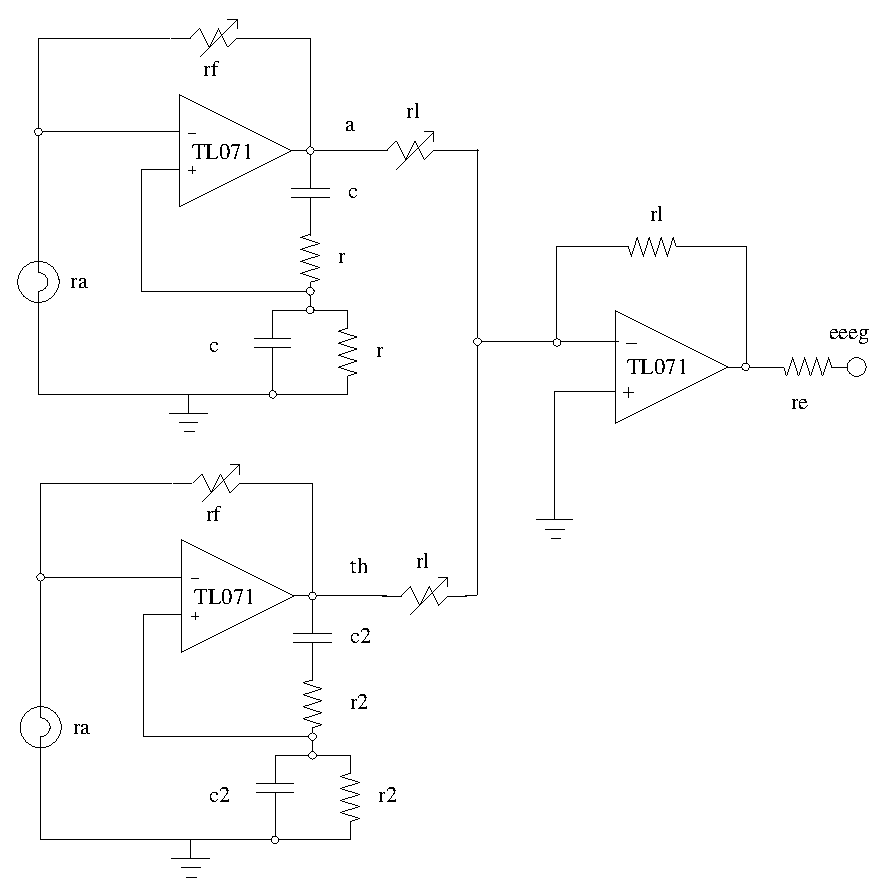
\includegraphics[width=\textwidth]{eeeg.eps}
    \caption{$e_{EEG}$ integration.}
    \label{fig:eeeg}
	\end{center}
\end{figure}

Figure~\vref{fig:eeeg} illustrates how $e_b$ is implemented using one
or more of the Wein--bridge oscillators described in
Section~\ref{section:sin}. In Figure~\vref{fig:eeeg} only the $\alpha$
and $\beta$ signals are summed to produce $e_{EEG}$. The $e_{EEG}$
signal is the sum of the voltages $\alpha$ and $\beta$ weighted by the
reciprocals of their input resistance values. By varying the input
resistors the contribution of each input signal to $e_{EEG}$ is
changed to reflect the signal voltage values specified in
Table~\vref{table:test-pros}.



The $e_{EEG}$ signal has a very low output impedance as can be
expected from the operational amplifier output stage of the adder
circuit. A 10~k$\Omega$ series resistance $r_e$ is added in order to
emulate the cranial impedance of a real human head. The addition of
$r_e$ makes it possible to use the SME as a general test bench. 

The purely resistive model of cranial impedance ($r_e$) used in the
SME is considered to be adequate for the bandwidth under
investigation. Phase errors and reactive impedance introduced by the
skin is considered small enough to be neglected. The SME can therefore
not be used for high--frequency skin or bone impedance measurements.

\begin{table}
\begin{center}	
	\begin{tabular}[htpb]{|l|l|} \hline
	$C$ & 2~$\mu$F \\
	$R_{\alpha}$ & 6.7~k$\Omega$ \\
	$R_{\beta}$ & 4.4~k$\Omega$ \\
	$R_e$ & 10~k$\Omega$ \\
	$R_l$ & 10~k$\Omega$ \\
	$trim$ & 0 -- 1~k$\Omega$ \\
	\hline
	\end{tabular}
	\caption{$e_{EEG}$ generator component values}
	\label{table:eeg-val}
\end{center}	
\end{table}

Table~\vref{table:eeg-val} summarizes the component values used in the
$e_{EEG}$ generator implementation.


\section{$e_c$ integration}
\begin{figure}[htbp]
	\begin{center}
	\psfrag{rf}{$trim$}
	\psfrag{r}{$R_{50Hz}$}
	\psfrag{rl}{$R_l$}
	\psfrag{r2}{$R_2$}
	\psfrag{c}{$C$}
	\psfrag{int}{$e_{cs}$}
	\psfrag{ecn}{$e_{s}$}	
	\psfrag{ew}{$e_{white}$}
	\psfrag{ec}{$e_c$}
	\psfrag{ra}{$lamp$}
	\psfrag{TL071}[][]{071}
	\psfrag{+}{+}
	\psfrag{-}{--}
	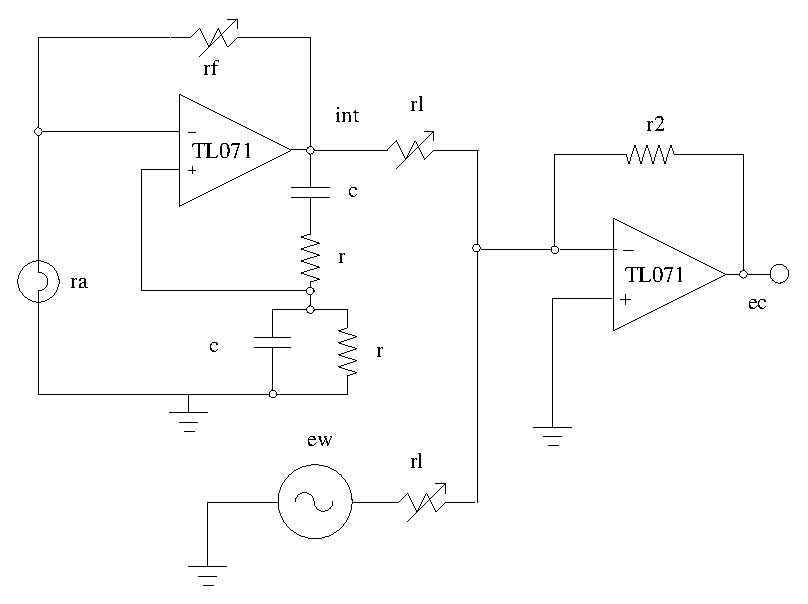
\includegraphics[width=\textwidth]{ec-int.eps}
    \caption{$e_c(t) = e_{sn} + e_{white}$.}
    \label{fig:ec-int}
	\end{center}
\end{figure}

The common mode signal $e_c$ is the sum of the sinusoidal signal
$e_{ns}$ and the white noise signal $e_{white}$. $e_{ns}$ is
implemented using the Wein-bridge circuit of
Section~\ref{section:wein} on page \pageref{section:wein}. The
$e_{cs}$ signal represents power line interference, the circuit of
Figure~\vref{fig:ec-int} oscillates at 50~Hz for the given resistance
value of 1.6~k$\Omega$.  $e_{white}$ is implemented using the circuit
described in Section~\ref{section:noise}.

The noise signal $e_{white}$ is added to $e_{ns}$ using the standard
operational amplifier summing circuit of Figure~\vref{fig:ec-int}. The
$R_l$ input resistances (0--20~k$\Omega$) is varied to adjust the
contribution of $e_{white}$ and $e_{cs}$ to the common mode signal
$e_c$.

\begin{table}
\begin{center}	
	\begin{tabular}[htpb]{|l|l|} \hline
	$C$ & 2~$\mu$F \\
	$R_{50Hz}$ & 1.6~k$\Omega$ \\
	$R_2$ & 10~k$\Omega$ \\
	$R_l$ & 0 -- 20~k$\Omega$ \\
	$trim$ & 0 -- 1~k$\Omega$ \\
	\hline
	\end{tabular}
	\caption{$e_c$ generator component values}
	\label{table:ec-val}
\end{center}	
\end{table}

Table~\vref{table:ec-val} summarizes the component values used in the
$e_c$ generator implementation.



\section{SME simulation}
The various signal sources used in the SME implementation are
simulated in order to facilitate the visual inspection of generator
outputs. As all signals in the SME are linearly summed it is necessary
to ensure that composite signal amplitudes does not drive the various
active components into non--linear regions distorting the test
signal. Source signal amplitudes are adjusted to ensure a linear SME
signal source. The signal simulations are used to accurately predict
and set maximum signal amplitudes.

\subsection{$e_b$ simulation}

\begin{figure}[htbp]
\begin{center}
	\psfrag{t}{time [s]}
	\psfrag{eb}[][]{$e_b$ [$\mu$V]}
	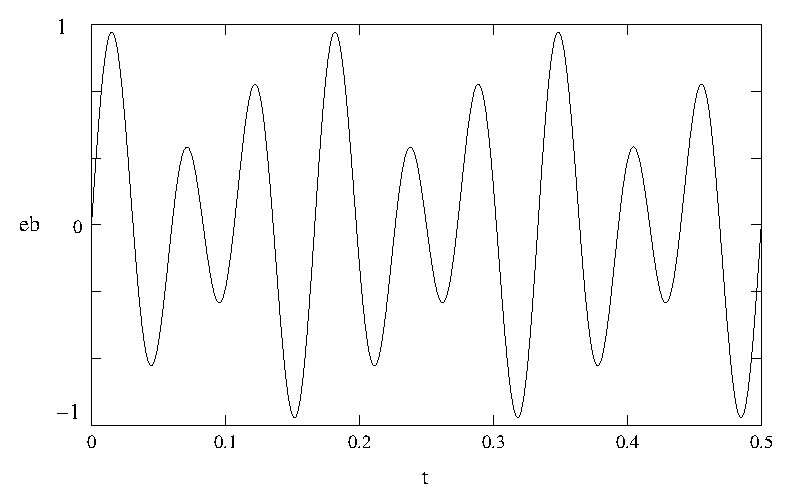
\includegraphics[width=\textwidth]{eb-sim.eps}
    \caption{$e_b(t)_{\alpha + \beta}$ simulation.}
    \label{fig:eb-sim}
\end{center}
\end{figure}

Figure~\vref{fig:eb-sim} depicts the normalized output of the
composite $e_b$ signal source set at the specified $\alpha$ and
$\beta$ frequencies.

\begin{equation} \label{eq:theta-sim}
	e_b(t)_{\alpha + \beta} = A_{\alpha}\sin\/(2\pi\alpha\/t) +
	A_{\beta}\sin\/(2\pi\beta\/t)
\end{equation}

$A_{\alpha}$ and $A_{\beta}$ are specified in
Table~\vref{table:test-pros}.

The power spectrum of Figure~\vref{fig:sme-eeg-power} is a averaged
signal and does not reflect the instantaneous power of a frequency
component. It is however prudent to note that the S/N ratio of the
$\gamma$ signal (40~Hz) is very low as the average amplitude of a
$\gamma$ band signal is $<2\mu\/V$. It would therefore be inaccurate
to use a high amplitude $\gamma$ frequency signal as a standard SME
test signal.


\subsection{$e_c$ simulation}

\begin{figure}[htbp]
\begin{center}
	\psfrag{t}{time [s]}
	\psfrag{ec}[][]{$e_c$ [$\mu$V]}
	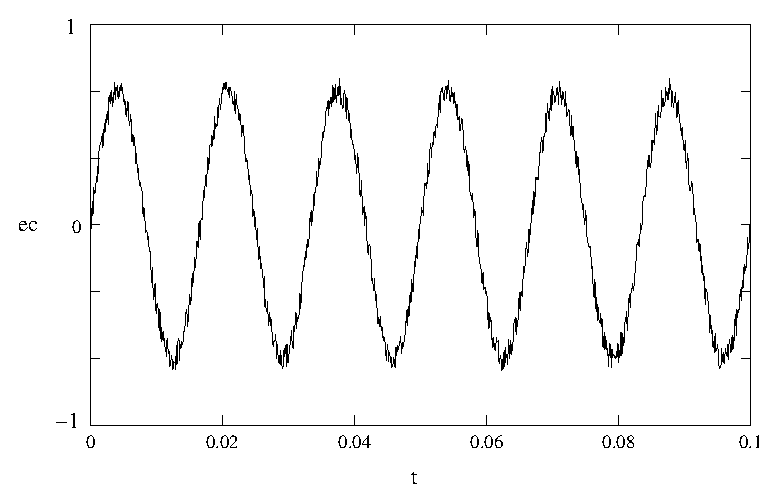
\includegraphics[width=\textwidth]{ec-sim.eps}
    \caption{$e_c(t)$ simulation.}
    \label{fig:ec-sim}
\end{center}
\end{figure}

Figure~\vref{fig:ec-sim} describes the normalized common mode signal
$e_c$. The common mode signal is consists of a 50~Hz interference
signal and a random white noise signal $e_{white}$
\begin{equation} \label{eq:ec-sim}
	e_c(t) = A_{int}\sin\/(2\pi\/f_{int}\/t) + A_{white}(2rand(t)-1) 
\end{equation}

$A_{int}$ is the amplitude of the sinusoidal interference signal. The
$rand()$ function output is scaled symmetrically around zero and
weighted to approximately 10\% of the sinusoidal amplitude. The noise
signal represents wide band interference from sources like fluorescent
lights and high--power electrical equipment.


\section{SME measurements and characterization}

This section discusses the SME implementation and presents time and
spectrum graphs of all the sinusoidal signal generators used in the
standard measurement environment. Because component tolerances exist
the measured output signal does not correspond 100\% with the
calculated design value. This is more prevalent for the
higher--frequency sources. A explanation for this phenomenon might be
the fact that a low mean resistance value for the light--bulb was
used.

\subsection{$\delta$ source measurements}

\begin{figure}[htbp]
\begin{center}
	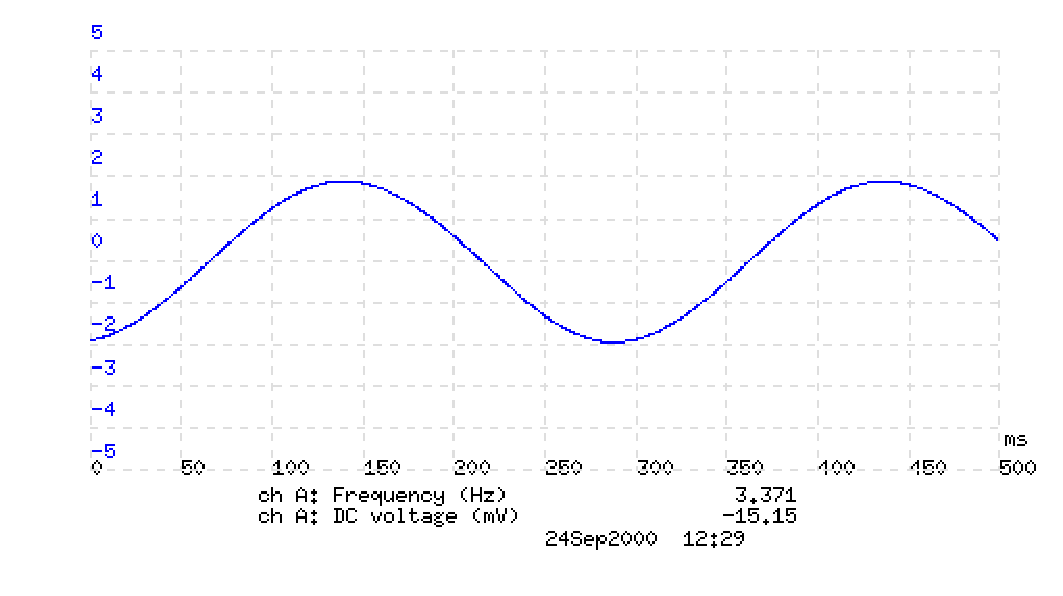
\includegraphics[width=\textwidth]{SME31.ps}
    \caption{SME 3~Hz ($\delta$) source time signal [V/ms]}
    \label{fig:sme3-1}
\end{center}
\end{figure}

Figure~\ref{fig:sme3-1} is a [V/time] trace as measured from the
output of the 3~Hz~($\delta$) SME sinusoidal signal generator. The
Y--axis represents volts. The realized $\delta$ frequency is 3.4~Hz
with a peak--to--peak amplitude of 3.78~V. A small -15.15~mV DC offset
is present. The measured frequency differs by $\pm$0.4~Hz from the
design value.

\begin{figure}[htbp]
\begin{center}
	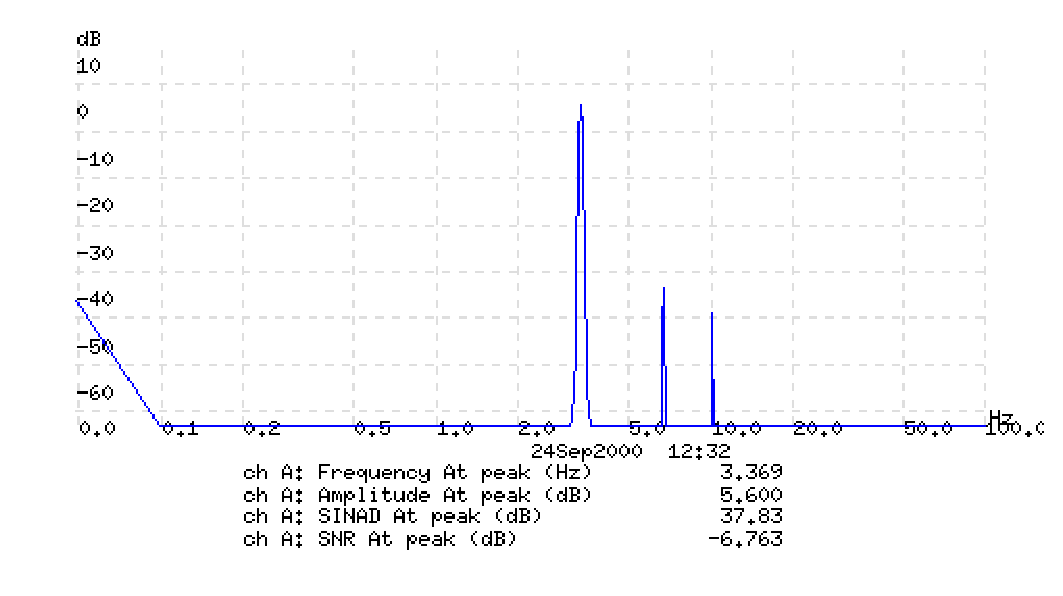
\includegraphics[width=\textwidth]{SME32.ps}
    \caption{SME 3~Hz ($\delta$) source spectrum [dB/Hz]}
    \label{fig:sme3-2}
\end{center}
\end{figure}

Figure~\ref{fig:sme3-2} is a [Power/frequency] trace as measured from
the output of the 3~Hz~($\delta$) SME sinusoidal signal generator. The
FFT was created by the PicoScope software package available from Pico
Technology Limited\footnote{http://www.picotech.com}. PicoScope is
shipped with the ADC-42 analog to digital conversion system used
during module and system testing and development. The software uses a
1~V value as the 0~dB reference.

A 2048 sample Hanning window was used to create the trace. The two
spikes to the right represents harmonies of the 3~Hz signal. A -35~dB
spike at approximately 6~Hz and a -44~dB spike at 9~Hz. Parasitic
capacitances in the circuit layout are believed to be responsible for
these spikes. It was first believed that the spikes were artifacts of
the FFT algorithm used but all of the windowing techniques available
in PicoScope delivered similar results.

The SINAD value mentioned at the bottom of Figure~\ref{fig:sme3-2} is
a ratio in dB of the signal plus noise plus distortion values to the
noise plus distortion values at the peak frequency:


\begin{equation} 
	SINAD = \frac{\sqrt{v_{rms-datum}^2 + v_{rms-1}^2 + v_{rms-2}^2 +
	...}}{\sqrt{v_{rms-1}^2 + v_{rms-2}^2 + ...}}
\label{eq:SINAD}
\end{equation}

The SINAD value is a measure of the quality of the signal. The
37.83~dB SINAD value reported by PicoScope was used to evaluate the
quality of the test signal as it progressed through the system.

\subsection{$\theta$ source measurements}

\begin{figure}[htbp]
\begin{center}
	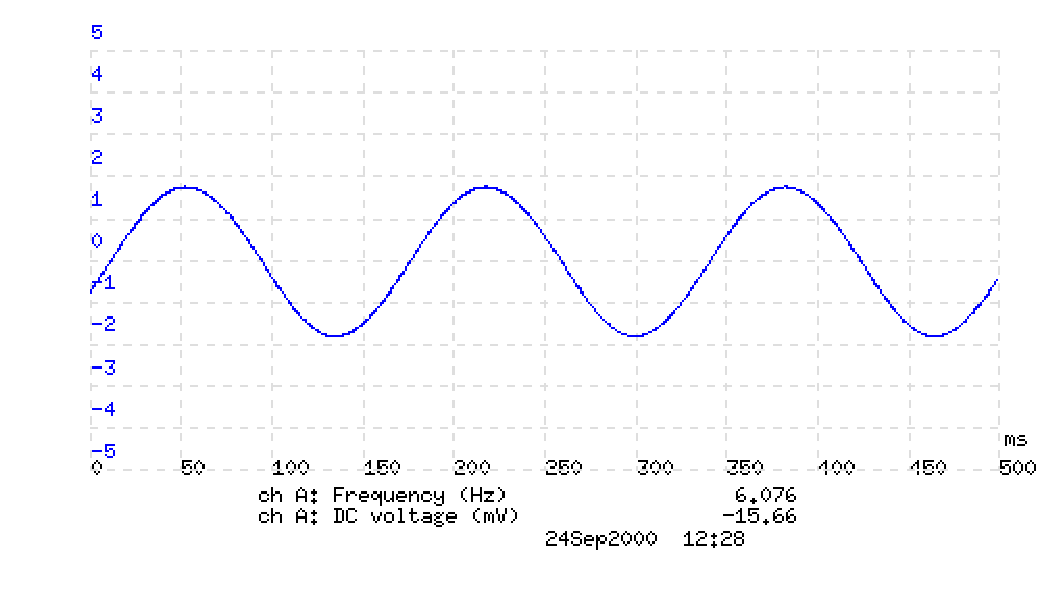
\includegraphics[width=\textwidth]{SME62.ps}
    \caption{SME 6~Hz ($\theta$) source time signal [V/time]}
    \label{fig:sme6-2}
\end{center}
\end{figure}

Figure~\ref{fig:sme6-2} is a [V/time] trace as measured from the
output of the 6~Hz~($\theta$) SME sinusoidal signal generator. The
Y--axis represents volts. The realized $\theta$ frequency is 6.1~Hz
with a peak--to--peak amplitude of 3.78~V. A small -15.66~mV DC offset
is present. The measured frequency differs by $\pm$0.1~Hz from the
design value.

\begin{figure}[htbp]
\begin{center}
	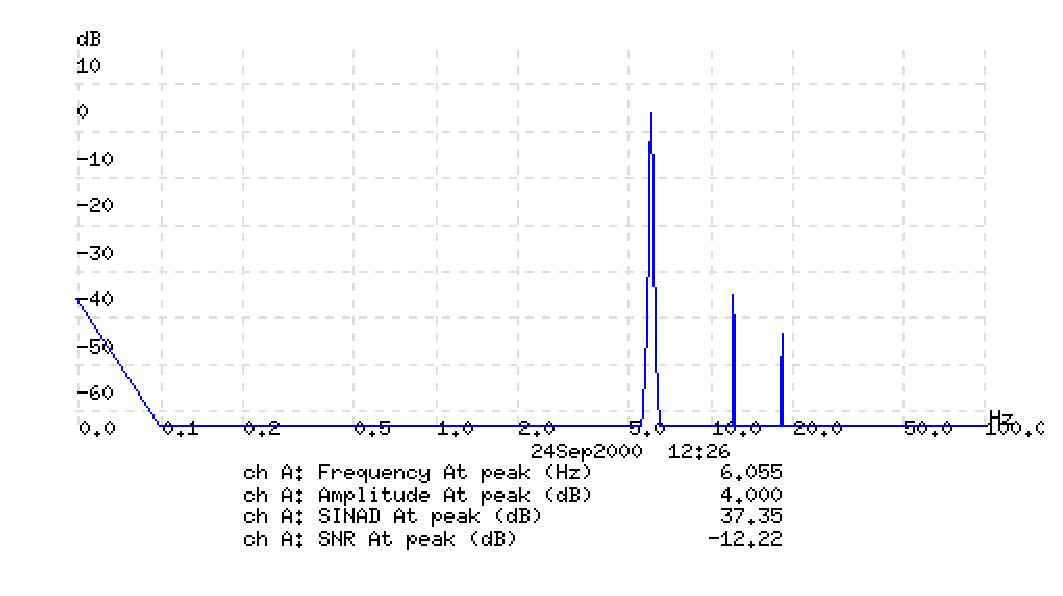
\includegraphics[width=\textwidth]{SME61.ps}
    \caption{SME 6~Hz ($\theta$) source spectrum [dB/Hz]}
    \label{fig:sme6-1}
\end{center}
\end{figure}


Figure~\ref{fig:sme6-1} is a [dB/Hz] trace as measured from the output
of the 6~Hz~($\theta$) SME sinusoidal signal generator.

A 2048 sample Hanning window was used to create the trace. The two
spikes to the right represents harmonies of the 6~Hz signal. A -35~dB
spike at approximately 12~Hz and a -45~dB spike at 18~Hz. Parasitic
capacitances in the circuit layout are believed to be responsible for
these spikes. It was first believed that the spikes were artifacts of
the FFT algorithm used but all of the windowing techniques available
in PicoScope delivered similar results.

\subsection{$\alpha$ source measurements}

\begin{figure}[htbp]
\begin{center}
	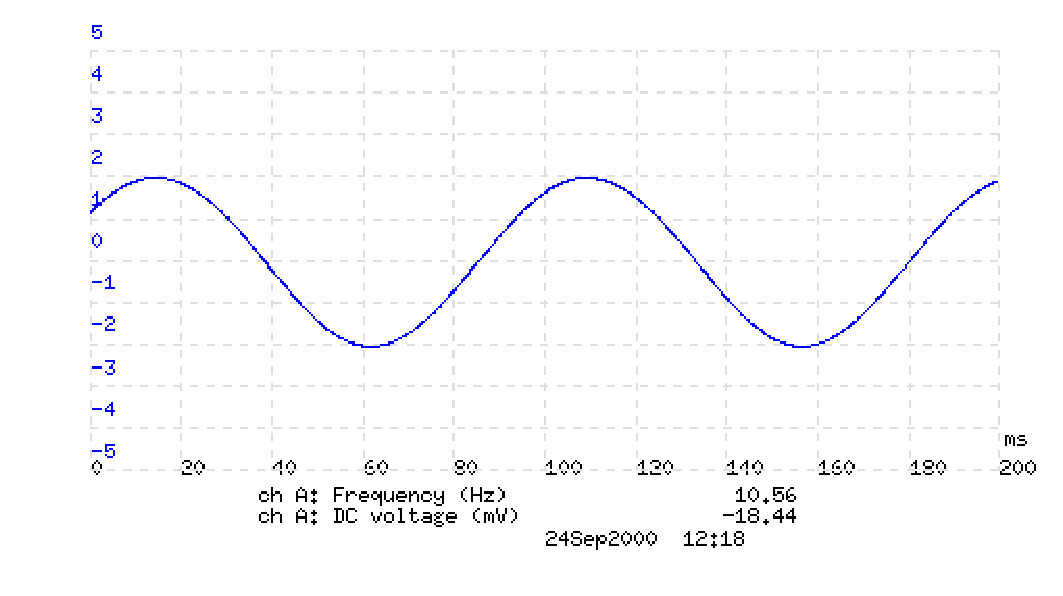
\includegraphics[width=\textwidth]{SME101.ps}
    \caption{SME 10~Hz ($\alpha$) source time signal [V/ms]}
    \label{fig:sme10-1}
\end{center}
\end{figure}

Figure~\ref{fig:sme10-1} is a [V/time] trace as measured from the
output of the 10~Hz~($\alpha$) SME sinusoidal signal generator. The
Y--axis represents volts. The realized $\alpha$ frequency is 10.5~Hz
with a peak--to--peak amplitude of 3.9~V. A small -18.44~mV DC offset
is present. The measured frequency differs by $\pm$2~Hz from the
design value.

\begin{figure}[htbp]
\begin{center}
	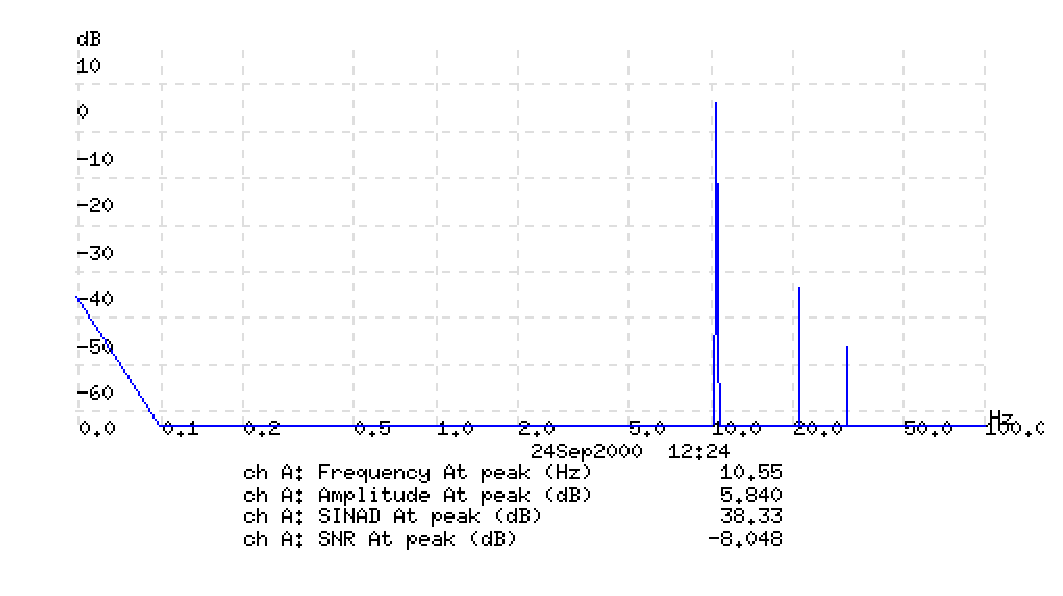
\includegraphics[width=\textwidth]{SME102.ps}
    \caption{SME 10~Hz ($\alpha$) source spectrum}
    \label{fig:sme10-2}
\end{center}
\end{figure}


Figure~\ref{fig:sme10-2} is a [Power/frequency] trace as measured from
the output of the 10~Hz~($\theta$) SME sinusoidal signal generator.

A 2048 sample Hanning window was used to create the trace. The two
spikes to the right represents harmonies of the 10~Hz signal. A -35~dB
spike at approximately 20~Hz and a -44~dB spike at 30~Hz. Parasitic
capacitances in the circuit layout are believed to be responsible for
these spikes. It was first believed that the spikes were artifacts of
the FFT algorithm used but all of the windowing techniques available
in PicoScope delivered similar results.

\subsection{$\beta$ source measurements}

\begin{figure}[htbp]
\begin{center}
	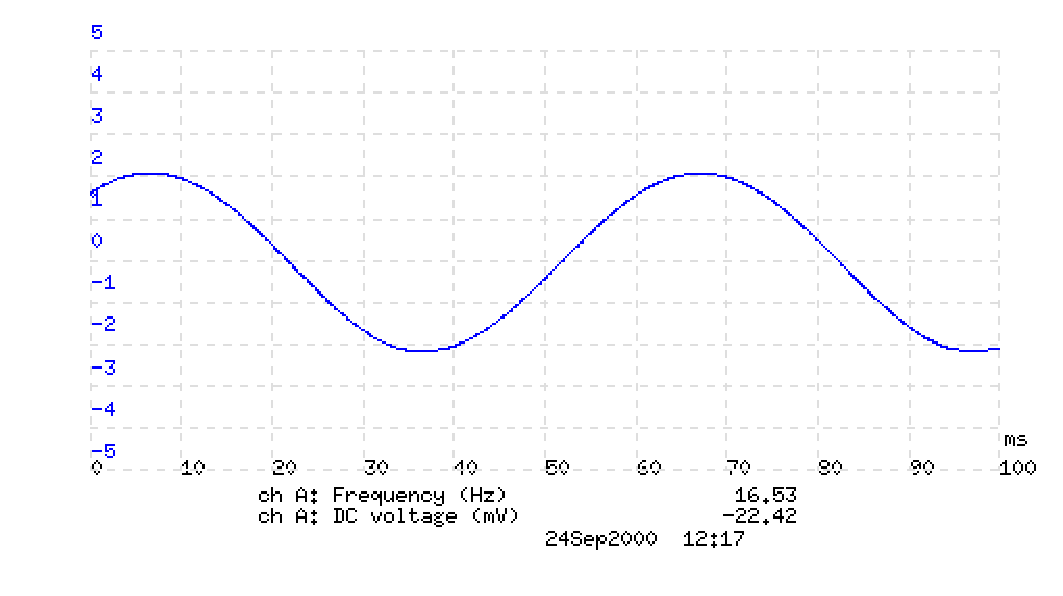
\includegraphics[width=\textwidth]{SME162.ps}
    \caption{SME 16~Hz ($\beta$) source time signal [V/time]}
    \label{fig:sme16-2}
\end{center}
\end{figure}

Figure~\ref{fig:sme16-2} is a [V/time] trace as measured from the
output of the 16~Hz~($\beta$) SME sinusoidal signal generator. The
Y--axis represents volts. The realized $\beta$ frequency is 16.5~Hz
with a peak--to--peak amplitude of 3.9~V. A small -22.42~mV DC offset
is present. The measured frequency differs by $\pm$1.5~Hz from the
design value.

\begin{figure}[htbp]
\begin{center}
	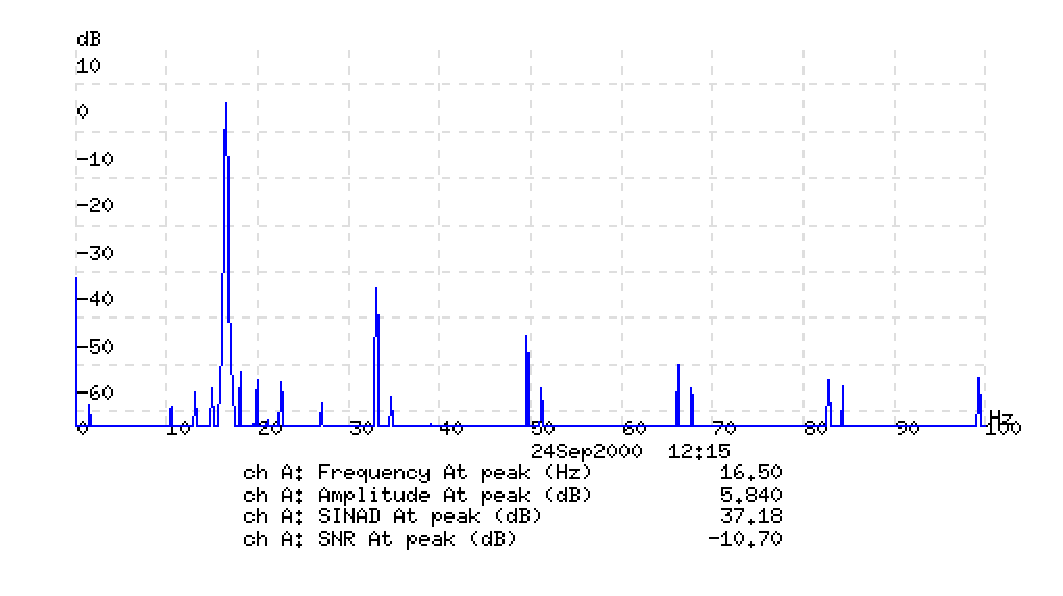
\includegraphics[width=\textwidth]{SME161.ps}
    \caption{SME 16~Hz ($\beta$) source spectrum}
    \label{fig:sme16-1}
\end{center}
\end{figure}

Figure~\ref{fig:sme16-1} is a [Power/frequency] trace as measured from
the output of the 16~Hz~($\beta$) SME sinusoidal signal generator.

A 1024 sample Hanning window was used to create the trace. The spikes
to the right represents harmonies of the 16~Hz signal. A -35~dB spike
at approximately 32~Hz and a -44~dB spike at 64~Hz are the higher
power harmonies. Parasitic capacitances in the circuit layout are
believed to be responsible for the high power spikes. The low power
spikes surrounding the base frequency and harmonies are artifacts of
the FFT algorithm used and a function of the width of the Hanning
window. In this case the window was chosen as 1024 samples, half that
of the previous measurements. Increasing the width of the window
increases the spectrum resolution and reduces algorithm artifacts at a
cost of increased computing time.


\subsection{$\gamma$ source measurements}

\begin{figure}[htbp]
\begin{center}
	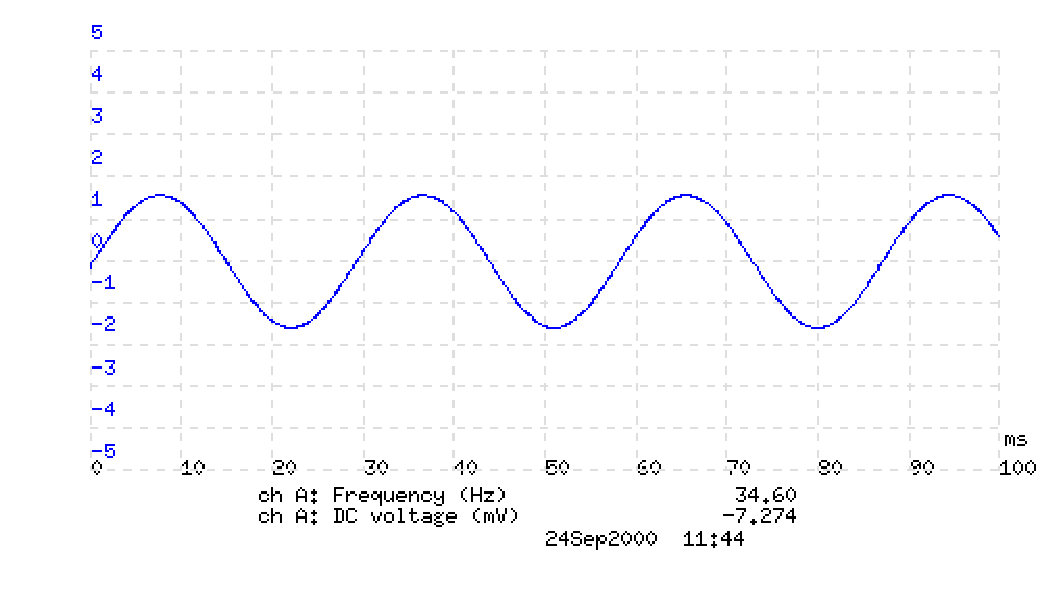
\includegraphics[width=\textwidth]{SME352.ps}
    \caption{SME 35~Hz ($\gamma$) source time signal [V/time]}
    \label{fig:sme35-2}
\end{center}
\end{figure}

Figure~\ref{fig:sme35-2} is a [V/time] trace as measured from the
output of the 35~Hz~($\gamma$) SME sinusoidal signal generator. The
Y--axis represents volts. The realized $\gamma$ frequency is 34.6~Hz
with a peak--to--peak amplitude of 3.6~V. A small -7.44~mV DC offset
is present. The measured frequency differs by $\pm$4.6~Hz from the
design value.


\begin{figure}[htbp]
\begin{center}
	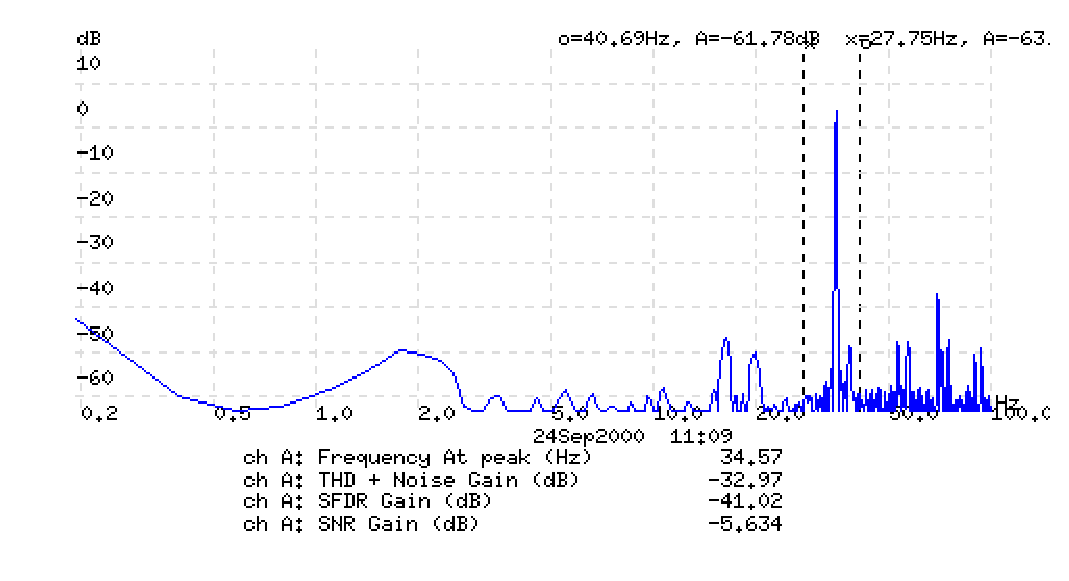
\includegraphics[width=\textwidth]{SME351.ps}
    \caption{SME 35~Hz ($\gamma$) source spectrum [dB/Hz]}
    \label{fig:sme35-1}
\end{center}
\end{figure}

Figure~\ref{fig:sme35-1} is a [dB/frequency] trace as measured from
the output of the 35~Hz~($\gamma$) SME sinusoidal signal generator.

A 1024 sample Hanning window was used to create the trace. The large
spike to the right (A -35~dB spike at approximately 70~Hz) is the
first multiple of the 35~Hz signal. Parasitic capacitances in the
circuit layout are believed to be responsible for the high power
spikes. The low power spikes surrounding the base frequency and
harmonies are artifacts of the FFT algorithm used and a function of
the width of the Hanning window. In this case the window was chosen as
1024 samples, half that of the previous measurements. Increasing the
width of the window increases the spectrum resolution and reduces
algorithm artifacts at a cost of computing time.


\begin{figure}[htbp]
\begin{center}
	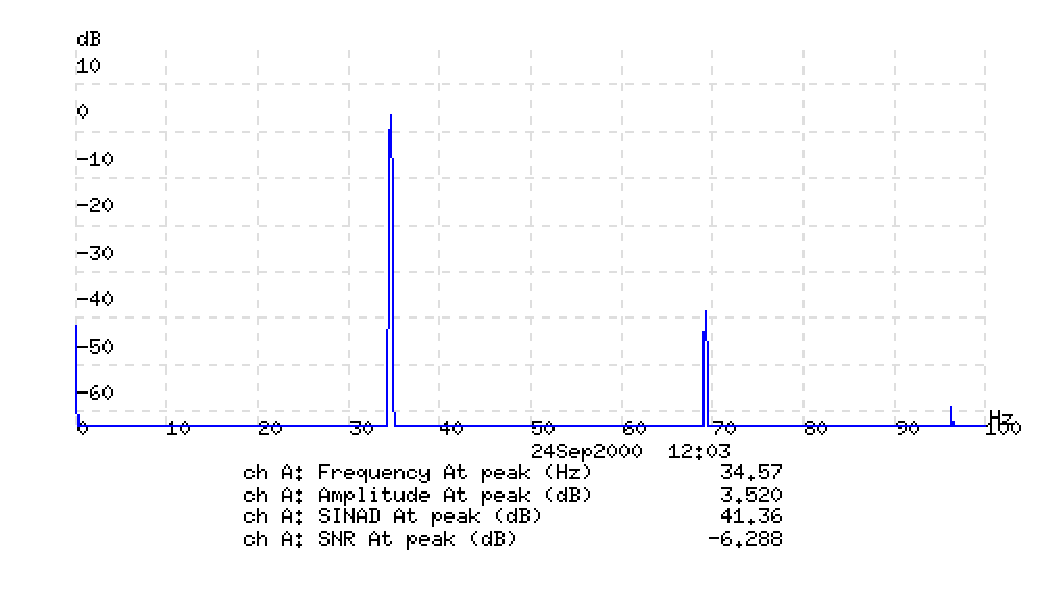
\includegraphics[width=\textwidth]{SME353.ps}
    \caption{SME 35~Hz $\gamma$ source spectrum [dB/Hz], 4096 Hanning window}
    \label{fig:sme35-3}
\end{center}
\end{figure}

Figure~\ref{fig:sme35-3} is reproduced as it illustrates a important
caveat when dealing with digital Fourier Transform (DFT)
implementations and their various algorithms. Figure~\ref{fig:sme35-3}
represents exactly the same signal as that of
Figure~\ref{fig:sme35-1}. The difference in representations are a
result of the width of the Hanning window used in creating the
result. Figure~\ref{fig:sme35-3} was created using a 4096 sample width
Hanning window, Figure~\ref{fig:sme35-1} used a 1024 width
window. Visual inspection of both graphs would imply that
Figure~\ref{fig:sme35-1} is more 'noisy' than
Figure~\ref{fig:sme35-3}, this assumption is false and may lead to a
incorrect interpretation of the signal trace.

\section{General Testing procedure} \label{section:test-proc}

The $\alpha$ signal from Table~\ref{table:test-pros} is used as the
standard test signal throughout the implementation of a specific
module. When it was deemed necessary other test frequencies were also
used. All test signals used were chosen from the signals specified in
Table~\ref{table:test-pros} and implemented using the Wein--bridge
oscillators previously discussed.




\chapter{Signal acquisition} \label{chap:sa}
%signal acquisition
%included in skripsie.tex

\section{Overview}

The signal acquisition module (SAM) captures all signals present on
the scalp surface and passes it on to the low--level signal processing
module's differential inputs. The signal acquisition module is
implemented using a set of active electrodes mounted on a removable
head--band.


The design and implementation of SAM entails the realization of the
physical electrodes as well as the electronic implementation of the
active electrode circuitry. The positioning of the device on the
cranium and the corresponding placement of the electrode's contact
surfaces is dependent on the design of the SAM container or
head--band. While all aspects of SAM design and implementation is
explored in some detail special consideration is given to noise
containment and elimination.


The goal of replacing passive electrodes with active devices implies a
redesign or enhancement of the standard passive electrodes as well as
their method of application. The traditional methods of reducing
electrode noise and motion artifacts are incompatible with the
high--level requirements of user friendliness and ease of use. 


Passive electrodes are the main injection point for external
interference into a EEG capturing system. By using active circuitry to
address the problems associated with traditional EEG electrodes the
noise and interference problems are addressed and the system's
usability enhanced.

\section{SAM design specification}

The signal acquisition module is required to produce a EEG signal of
at least comparative quality than that of current silver or gold
electrodes. The signal quality is defined in terms of noise present in
the output signal from the signal acquisition module. It is inevitable
that the active components of the active electrode will inject more
noise into the system that normal passive electrodes will. The
benefits derived from using a AE in terms of interference reduction
and greater CMRR due to reduced DC offset levels at the
instrumentation amplifiers input must compensate for the noise
injected by the active components.


The SAM submodule must also circumvent the current usability problems
associated with traditional electrodes.


The SAM must be able to deliver a low-noise EEG signal to the the
low-level signal processing module's (Chapter~\vref{chap:sa})
differential input stage. The EEG signal must be spectrally unaltered
in the band of interest (0.1~Hz~--~35~Hz) with a flat frequency
response within $\pm$0.5~dB of the source signal.


The SAM must also comply to the high--level design constraints set in
Table~\vref{table:hl-design-contraints}, that is a maximum permissible
application and adjust time of 10~s, a maximum removal time of 5~s and
no skin preparation.

The SAM design specification is logically sub-dived into a active
electrode and active electrode container specification:
\begin{itemize}
	\item{Active Electrode design specification} 
		\begin{itemize} 

			\item{The active electrode electronic design. Signal to
			noise ratio values, input and output impedances and the
			AE's transfer function are specified.}

			\item{The active electrode physical design dealing with
			physical aspects of the active electrode parameters including
			contact area and manufacturing processes.}

		\end{itemize}
	\item{Active Electrode container specification}
	
		\begin{itemize}
			\item{Specification of the montage protocol, and the degree of
			adjustment variability}
		\end{itemize}
\end{itemize}


Separating the design allows for the substitution of either designs or
subsequent implementations by another design or implementation for
comparative analysis. For example the contact area of the physical
electrode may be varied or the metal used in manufacturing may be
changed without changing the electronic design, and vice versa.


\subsection{AE electronic design specification}

In order to effectively develop the AE electronic design specification
cognizance must be taken of noise and interference problems
experienced when using traditional passive electrodes.

\subsubsection{Noise and interference analyses of passive electrodes}
\label{section:passive-analyses}
\begin{figure}[htb]
	\begin{center}
	\psfrag{eeg}{$e_{EEG}$}
	\psfrag{re}{$R_e$} 
	\psfrag{rc}{$R_c$} 
	\psfrag{cc}{$C_c$}
	\psfrag{rsg}[][]{$R_{sg}$}
	\psfrag{rsg}[][]{\colorbox{white}{$R_{sg}$}}
	\psfrag{electrolyte}{Electrolyte}
	\psfrag{movement}{Movement}  
	\psfrag{emi}[][]{EM interference}
	\psfrag{fields}{fields}  
	\psfrag{stratum granulosum}{\em stratum granulosum \em}  
	\psfrag{soft tissue}{Soft tissue}
	\psfrag{cranium}{Cranium}
	\psfrag{Brain}{Brain}
	\psfrag{metal}{Metal}
	\psfrag{contaminant}{Contaminant}
	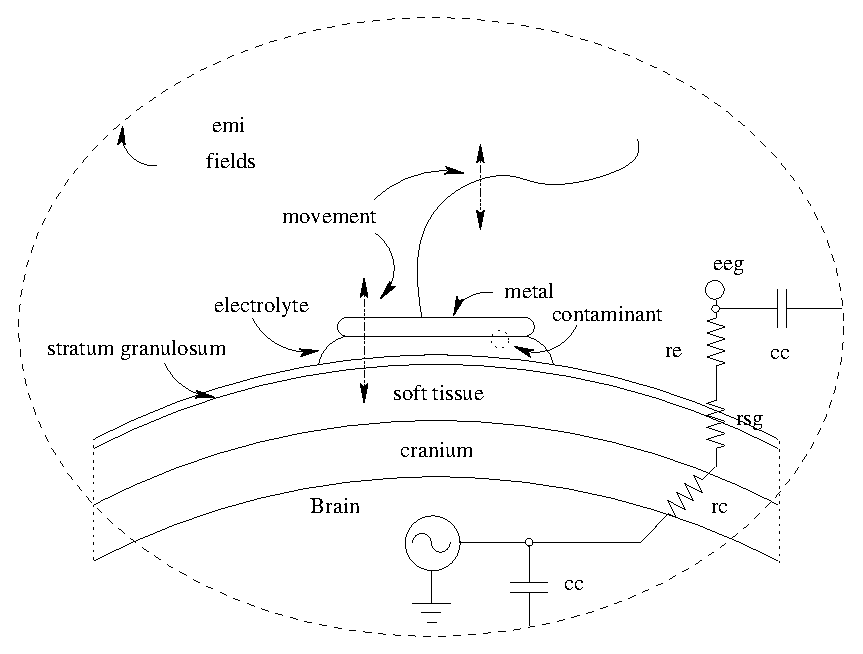
\includegraphics[width=\textwidth]{electrode-noise.eps}
	\caption{Passive electrode noise sources}
	\label{fig:electrode-noise} 
	\end{center}
\end{figure}


Electrodes are subject to a range of interference and noise.
Figure~\vref{fig:electrode-noise} depicts a traditional passive
electrode applied to the scalp surface using electrolytic gel. Various
noise and interference sources are shown at their individual injection
points. The cranial resistance $R_c$ and \em stratum granulosum \em
resistance $R_{sg}$ is lumped together as the skin resistance
$R_{skin}$. $R_c$ is small in comparison with $R_{sg}$ and is usually
ignored.


Traditionally electrodes are applied to carefully prepared surfaces on
the subject's skin. A major source of signal artifacts is the
potential difference ($e_{sg}$) between the outer and inner layers of
\em stratum granulosum \em of the human scalp. The $e_{sg}$ potential has a
magnitude of around 30~mV \cite{reducing-motion-artifacts} and varies
according to the mechanical stress exerted on the skin. Any electrode
movement is directly translated into a movement artifact. Preparing
the skin by removing the top layer of dead isolating skin cells
effectively reduces the $e_{sg}$ potential to a negligible value
\cite{reducing-motion-artifacts}. 


The \em stratum granulosum \em is responsible for the dominant
component of human skin resistance at 10--100~k$\Omega$/cm$^{2}$
\cite{active-electrode-ca}. The skin resistance acts as part of the
voltage divider circuit attenuating the EEG signal amplitude when
measured with a low--input impedance device. 


Electrodes can induce large motion artifacts due to physical movement
of the electrical double layer that forms at the electrolyte--metal
interface \cite{reducing-motion-artifacts}.  Electrode--electrolyte
induced artifacts have a amplitude of approximately 15~mV depending on
the metal being used. The use of electrolyte permits a secure and
relatively constant impedance between electrode and skin surfaces. The
electrode gel ensures the availability of conductive ions and isolates
the metal electrode from foreign substances. The effective conduction
area and signal conduction path characteristics are also kept
constant. A variation in the electrode conduction area and its
effective resistance translates into a signal artifact in the measured
signal \cite{reducing-motion-artifacts}.


Another source of electrode noise is the electrode's potential
stability. Small contamination of foreign substances on electrode
surfaces can lead to large fluctuating signal potentials of up to 1~mV
\cite{electrode-stability}. The contaminating metal and electrode
effectively constitutes a short-circuited electro-chemical cell that
induces a localized current into the electrolyte surrounding the cell,
leading to spurious signal artifacts.


Mains power line interference enters the system via the connecting
electrode cables. Triboelectric cable noise is caused by the resulting
friction and deformation of the cable isolation during cable
movement. Long cables which are physically far from the body also
increases the effective area exposed to power line induced magnetic
fields. The magnetic field passes through the loop created by the
cable and body and induces current flow in the circuit
\cite{reducing-motion-artifacts}. The current flow translates to a large
common mode 50~Hz interference signal.


Power line induced 50~Hz interference usually constitutes the largest
amplitude component of the common mode signal seen from the
differential inputs of a instrumentation amplifier. Other large common
mode signal components are introduced by fluorescent lights which
radiates at factors of the power line frequency. External
electromagnetic interference sources are capacitively (via $C_c$ of
Figure~\vref{fig:electrode-noise}) coupled into the system at various
points.

Having identified the major sources of noise and interference in
passive electrodes it is now possible to specify active electrode
circuit characteristics curbing the impact of contamination on signal
quality. Noise reduction techniques can now be employed to reduce the
noise levels to the lowest possible level.


\subsubsection{AE electronic specification synopsis}
If the input impedance of the electrode ($R_e$) is more than 100 times
larger than that of $R_{skin}$ the preparation of the skin surface and
the application of electrode gel to enhance signal conduction becomes
largely unnecessary. A low electrode output impedance will reduce
environment noise introduced in the lead cables. The active electrode
must have a high input impedance and a low output impedance.


At every electrode a contact potential is generated between the
electrode--electrolyte layer, the ever present mixture of sweat and
normal skin secretions acts as a electrolyte.  When using similar
materials the electrode offset potentials are in the same order but
very seldom equivalent
\cite{buffer}. The active electrode must be capable of negating
relatively large DC offset values thus enabling the differential
amplifier of the the low--level signal processing module to have a
gain setting of at least 80~dB without fear of saturation.


\subsection{AE physical design specification}

Bio--compatibility requires that the material used on the surface of
the electrode be non--toxic and capable of withstanding the harsh
chemical conditions of the normal human skin. This material must also
be cost effective and easily replaceable with more traditional
electrodes. This aspect of the electrode design enables the comparison
of noise and impedance figures with that of traditional passive
electrodes.


Since the cranial surface potential is a superposition of potentials
induced by a great number of nerve fibers, the size of the electrode
will influence the EEG signal strength. A large electrode will yield a
stronger signal with a comparable loss in resolution, and vice
versa. The placement of the various electrodes will also influence the
size of an individual electrode. The electrode material must also be
electrically suitable, exhibiting low material--contamination noise
characteristics \cite{electrode-stability}.

\subsection{SAM container specification}
The electrodes must be contained in a semi--rigid array to ensure
constant relative electrode positions for different electrode
configuration measurements (mono-polar, bipolar etc.). This suggests a
headset or head--band. The container must be able to apply the
electrode contact areas with equal and constant pressure unto the skin
surface reducing motion artifacts and keeping skin impedance constant.

\section{SAM  implementation}
\subsection{Active electrode implementation}
\label{section:ae-imp}
In order to effectively design and implement an active electrode it is
necessary to note the relevant characteristics of the devices
receiving the active electrode output signal.

\begin{figure}[htbp]
	\begin{center}
	\psfrag{ze1}{$Z_{e1}$}
	\psfrag{ze2}{$Z_{e2}$}
	\psfrag{a}{$a$}
	\psfrag{b}{$b$}
	\psfrag{zc1}{$Z_{c1}$}
	\psfrag{zc2}{$Z_{c2}$}
	\psfrag{zd}{$Z_d$}
	\psfrag{rs1}{$R_{s1}$}
	\psfrag{rs2}{$R_{s2}$}
	\psfrag{vc}{$V_c$}
	\psfrag{+}{+}
	\psfrag{-}{--}
	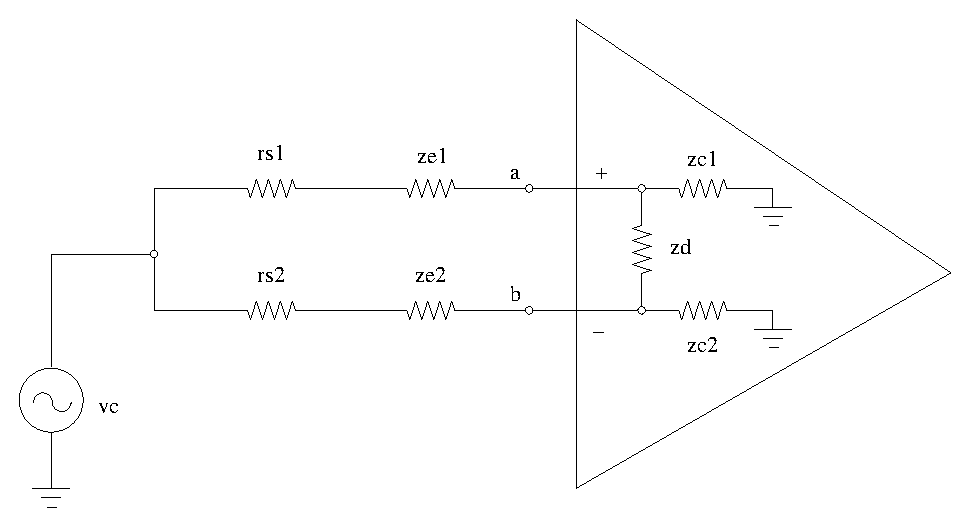
\includegraphics[width=\textwidth]{diff-amp-frontend.eps}
	\caption{ Differential amplifier input}
	\label{fig:diff-amp-frontend}
	\end{center}
\end{figure}

Figure~\vref{fig:diff-amp-frontend} represents the EEG signal path
from the skin surface to the inputs of a differential
amplifier. Figure~\vref{fig:diff-amp-frontend} extends
Figure~\vref{fig:sme-eq} to include the input impedances of the
receiving amplifiers front end. $Z_{e1}$ and $Z_{e2}$ are electrode
impedances, $Z_{c1}$ and $Z_{c2}$ are the common mode amplifier
impedances and $Z_d$ the differential mode amplifier impedance. Any
difference between either $R_{s1}$ -- $R_{s2}$, $Z_{e1}$ -- $Z_{e2}$
or $Z_{c1}$ -- $Z_{c2}$ translates into a false differential signal
voltage over $Z_d$. In commercial instrumentation amplifier (IA)
packages, $Z_{c1}$ and $Z_{c2}$ are usually the non--inverting inputs
of balanced on--chip operational amplifiers. Because the input
impedances of the buffer amplifiers used in IA's are very high the
erroneous differential signal introduced by variations between the
impedance pairs $Z_{c1}$ -- $Z_{c2}$ and $R_{s1}$ -- $R_{s2}$ are
greatly reduced \cite{buffer}.

Due to the low order of EEG signals (1--100~$\mu$Vpp at 0.1--35~Hz)
at the cranial surface) \cite{intro-to-bio} and the fact that
unprepared skin surfaces are used, all possible precautions to prevent
EEG signal attenuation and noise contamination is considered and
implemented where possible.

If the input impedance of the electrode is very high ($>$10M~$\Omega$)
and the output impedance very low ($<$1~$\Omega$) the active electrode
acts as a impedance transformer negating the need for surface
preparation \cite{active-electrode-ca}. The active electrode must be
AC coupled in order to remove electrode offset potentials and allow for
a high gain differential stage in the low level signal processing
module \cite{buffer}.

\subsubsection{Active electrode circuit design and analysis}
\begin{figure}[htbp]
	\begin{center}
	\psfrag{+}{+}		
	\psfrag{-}{--}		
	\psfrag{a}{$a$}		
	\psfrag{b}{$b$}		
	\psfrag{v1}{$v_i$}		
	\psfrag{vo}{$v_o$}		
	\psfrag{c2}{$C_2$}		
	\psfrag{r1}{$R_1$}		
	\psfrag{r2}{$R_2$}		
	\psfrag{c1}{$C_1$}		
	\psfrag{va}{$V_a$}		
	\psfrag{vb}{$V_b$}		
	\psfrag{TL071}[][]{071}
	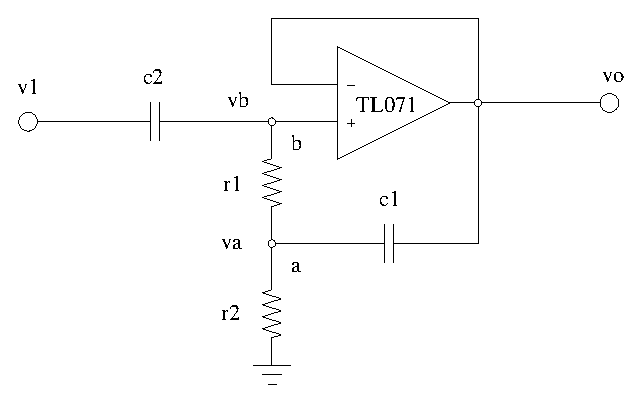
\includegraphics[]{active-electrode.eps}
	\caption{Active electrode circuit diagram \cite{buffer}}
	\label{fig:active-electrode}
	\end{center}
\end{figure}
The active electrode specification requirements are satisfied by using
a FET--input operational amplifier in the bootstrapped voltage
follower circuit of Figure~\vref{fig:active-electrode} as the active
electrode buffer circuitry.

Capacitor $C_2$ Figure~\vref{fig:active-electrode} decouples any DC
components of the input voltage $v_i$. The inclusion of $C_2$ enables
the active electrode to deliver a AC signal to the differential
amplifier inputs of the low level signal processing module. For a
low--noise design it is important to have the highest gain possible
concentrated in the first amplifier stage of the system
\cite{buffer}. If the applied signals have no DC offsets the
differential stage gain may be set to 60~dB or more without amplifier
saturation problems. The inclusion of $C_2$ makes the addition of a
bias current path mandatory. The bias path can compromise the high
input impedance of the operational amplifier input, negating the
primary benefit of using a operational amplifier as active
electrode. The inclusion of $C_1$ in the bias path enables $R_1$ to
act as a high impedance current source to $v_i$ restoring the input
impedance. Reducing the value of $C_2$ because it feeds a
high-impedance load may lead to unwanted peaks in the AE frequency
response, distorting the measured EEG signal, \cite[p183-184]{art}.

\subsubsection{Active electrode transfer function}
The transfer function of the active electrode circuit of
Figure~\vref{fig:active-electrode} is deduced by summing currents at
nodes $a$ and $b$ and noting the closed loop voltage gain.
\begin{equation}
	\frac{V_a - V_b}{R_1} + \frac{V_a}{R_2} = (v_o - V_a)sC_1
	\label{eq:node-a}
\end{equation}
\begin{equation}
	(V_b - v_i)sC_2 = \frac{V_a - V_b}{R_1}
	\label{eq:node-b}
\end{equation}
With $A_o >> 1$ the open loop gain of the operational amplifier and
$\omega_a$ the corner frequency:
\begin{equation}
	\frac{(V_b - v_o)A_o\omega_a}{s + \omega_a} = v_o
	\label{eq:gain}
\end{equation}
The time constants are defined as follows:
\begin{equation}
	\tau_1 = \frac{R_1\/R_2}{R_1 + R_2}C_1
	\label{eq:tau1}
\end{equation}
\begin{equation}
	\tau_2 = (R_1 + R_2)C_2
	\label{eq:tau2}
\end{equation}
\begin{equation}
	\tau_m = R_2\/C_2
\end{equation}
\begin{equation}
	\tau_a = \frac{1}{\omega_a}
\end{equation}
\begin{equation}
	\tau^2_n = R_1\/R_2\/C_1\/C_2 = \tau_1\/\tau_2
\end{equation}
The active electrode transfer function in terms of input and output
signal voltage is:
\begin{equation}
	\frac{v_o(s)}{v_i(s)} = 
	\frac{s\tau_2(1 + \frac{\tau_1}{s})}{1 + s[\tau_2 + \frac{\tau_m +
	\tau_a}{A_o}] + s^2[\tau^2_n + \frac{\tau_a(\tau_m + \tau_2)}{A_o}] +
	s^3\frac{\tau^2_n\tau_a}{A_o}}
	\label{eq:trans}
\end{equation}

From Equation~\ref{eq:trans} can be seen that the active electrode is
a unity gain voltage follower only at low frequencies excluding
DC. Equation~\ref{eq:trans} can be simplified for low frequencies by
choosing time constant values reducing all terms containing $A_o$ to
insignificant values. For frequencies below the $A_o$ containing terms
in the transfer function denominator the active electrode transfer
function is reduced to:

\begin{equation}
	H(s) = \frac{v_o(s)}{v_i(s)} = \frac{s(s+\frac{1}{\tau_1})}{s^2 +
	\frac{s}{\tau_1} + \frac{1}{\tau_1\/\tau_2}}
\label{eq:simp-trans}
\end{equation}
The damping factor $\epsilon$ for $H(s)$ is given by : 
\begin{equation}
	\epsilon = \frac{(\tau_1/\tau_2)^\frac{1}{2}}{2}
\end{equation}

\begin{figure}[htbp]
	\begin{center}
	\psfrag{tau1}{$\tau_1$}		
	\psfrag{tau2}{$\tau_2$}		
	\psfrag{eps}{$\epsilon$}		
	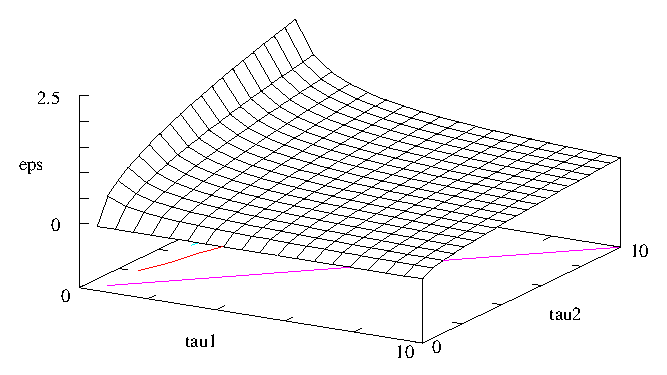
\includegraphics[width=\textwidth]{damping.eps}
	\caption{$\epsilon(\tau_1, \tau_2)$}
	\label{fig:damping}
	\end{center}
\end{figure}

Figure~\vref{fig:damping} plots the damping factor $\epsilon$ as a
function of the time constants $\tau_1$ and
$\tau_2$. Figure~\vref{fig:damping} illustrates the damping factors
greater variance with respect to $\tau_2$ for relatively low $\tau_1$
values. In order to reduce overshoot at $\omega_n$ to acceptable
levels $\tau_1$ and $\tau_2$ values must result in a moderate
$\epsilon$ surface slope.


The natural frequency $\omega_n$ is:
\begin{equation}
	\omega_n = (1/\tau_1\/\tau_2)^\frac{1}{2} = 1/\tau_n
	\label{eq:wn}
\end{equation}

\begin{figure}[htbp]
	\psfrag{tau1}{$\tau_1$}		
	\psfrag{tau2}{$\tau_2$}		
	\psfrag{wn}{$\omega_n$}		
	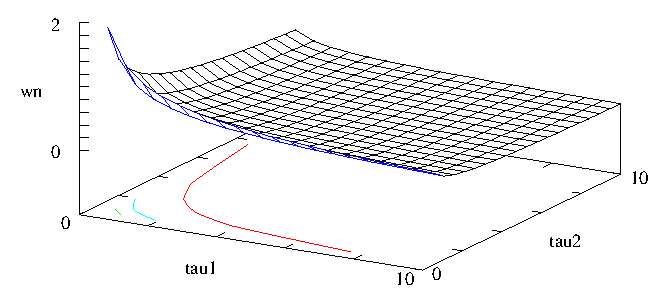
\includegraphics[width=\textwidth]{natural.eps}
	\caption{$\omega_n(\tau_1, \tau_2)$}
	\label{fig:natural}
\end{figure}

Figure~\vref{fig:natural} plots the natural frequency $\omega_n$ as a
function of the time constants $\tau_1$ and $\tau_2$.

The active electrode acts as a high--pass filter for low frequencies,
the amount of overshoot at the natural frequency $\omega_n$ is
determined by the damping factor $\epsilon$.  $\tau_1$ and $\tau_2$
are specified by the values of $C_2$, $C_1$, $R_1$ and $R_2$, see
Equations~\ref{eq:tau1} and \ref{eq:tau2}. The frequency response in
the band of interest must be flat within $\pm$0.5~dB over the
0.1~--~35~Hz range.

Input impedance must remain high and the effect of $\tau_1$ and
$\tau_2$ on the active electrode input impedance must be understood
before specifying time constant values.

\subsubsection{Active electrode input impedance}
Noting the signal current flowing into $C_2$ the active electrode
impedance can be described as follows:
\begin{equation}
	Z = \frac{v_i}{(v_i - v_b)C_2s}
	\label{eq:z}
\end{equation}

Substituting the current Equations~\ref{eq:node-a} and \ref{eq:node-b}
into Equation~\ref{eq:z} and discarding high--frequency terms:
\begin{equation}
	Z = \frac{1 + s\tau_2^2 + s^2\tau_1\/\tau_2}{C_2s}
	\label{eq:z-long}
\end{equation}
substituting $\tau_1$ and $\tau_2$ with the component constants
yields:
\begin{equation}
	Z = \frac{1}{C_2s} + R_1 + R_2 + sR_1R_2C_1
	\label{eq:z-long2}
\end{equation}


\subsubsection{Design for optimal $\tau_1$ and $\tau_2$}
A active electrode must have a high input impedance as well as a flat
frequency response over the band of interest. $\tau_1$ and $\tau_2$
must therefore be designed to ensure that the overshoot at the natural
frequency $\omega_n$ and the attenuation at the low frequency side
does not go beyond the $\pm$0.5~dB specification.

To ensure a high input impedance for interference frequencies it is
necessary to design the electrode's transfer function to act
inductively in the interference frequency range. In general:
\begin{equation}
	R_1 + R_2 < \omega_{int}R_1R_2C_1
	\label{eq:wint}
\end{equation}
$\omega_{int}$ is the interference frequency signal. The modulus of
the transfer function $ \left | H(s) \right | = \left |
\frac{v_o(s)}{v_i(s)} \right | = 1$, at the frequency $\omega_l =
\frac{\omega_n}{\sqrt{2}}$. The same holds for frequencies larger than
the natural frequency $\omega_n$. The lowest frequency in the band of
interest must therefore not be below that of $\omega_l$.

The maximum amplitude of the transfer function $H(s)$ occurs at the
frequency $\omega_{max}$:
\begin{equation}
	\omega_{max} = \frac{\omega_n\sqrt{1 + \sqrt{1 +
	8\epsilon^2}}}{\sqrt{2}}
	\label{eq:omega-max}
\end{equation}
Substituting Equation~\ref{eq:omega-max} into the modulus of the
transfer function yields:
\begin{equation}
	\left | \frac{v_o(s)}{v_i(s)} \right | ^2 = \frac{1 + 8\epsilon^2 +
	(4\epsilon^2 + 1)\sqrt{1 + 8\epsilon^2}}{1 + 8\epsilon^2 +
	(4\epsilon^2 - 1)\sqrt{1 + 8\epsilon^2}}
	\label{eq:max-mag}
\end{equation}

Equation~\ref{eq:max-mag} describes the maximum magnitude of the
transfer function at a specified damping factor $\epsilon$. The
magnitude of the overshoot ($\xi$) is the root of the maximum
magnitude - 1:
\begin{equation}
	\xi = \left | \frac{v_o(s)}{v_i(s)} \right | - 1
	\label{eq:overshoot}
\end{equation}

The rate of attenuation below $\omega_l$ is influenced by
$\epsilon$. The -3~dB frequency $\omega_{-3~dB}$ for $H(s)$
at a specified $\epsilon$ is:
\begin{equation}
	\omega_{-3dB} = \omega_n\sqrt{\sqrt{(2\epsilon^2 + 1) + 1} -
	(2\epsilon^2 + 1)}
	\label{eq:wm1}
\end{equation}

\begin{figure}[htbp]
	\begin{center}
	\psfrag{eps}{$\epsilon$}		
	\psfrag{-3db}{$\omega_{-3dB}$}		
	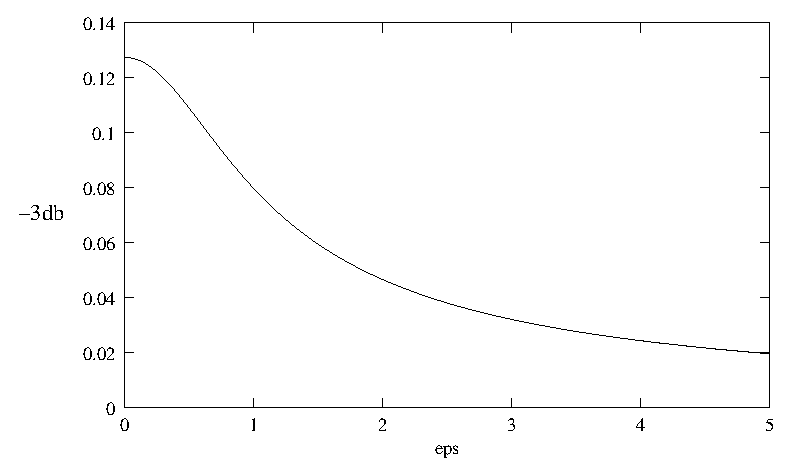
\includegraphics[width=\textwidth]{3db.eps}
	\caption{$\omega_{-3dB}(\epsilon)$}
	\label{fig:3db}
	\end{center}
\end{figure}

Figure~\vref{fig:3db} describes the system roll--off dependency on the
damping factor $\epsilon$. As $\epsilon$ increases the half--power
frequency $\omega_{-3dB}$ decreases. The time constant values must be
chosen to keep $\epsilon$ as small as possible while keeping the
pass--band overshoot within the $\pm$0.5~dB margin.

\subsubsection{Component value calculations}
\label{section:comp-values}
Applying the design equations described in the previous sections
allows for the effective selection of the active electrode component
values.

\begin{table}
\begin{center}	
	\begin{tabular}[htpb]{|c|c|c|c|} \hline
	Parameter & Value \\ \hline
	Minimum input impedance at 50~Hz & 100~M$\Omega$ \\
	Maximum resistor value & 10~M$\Omega$ \\ 
	$f_c$ & 0.1~Hz \\
	\hline
	\end{tabular}
	\caption{AE component specification parameters}
	\label{table:ae-specs}
\end{center}	
\end{table}

With the interference frequency $f_i$~=~50~Hz Equation~\ref{eq:wint}
becomes:

\begin{equation}
	R_1R_2C_1 = \frac{10^8}{100\pi} 
\end{equation}

From Equation~\ref{eq:wn} and $\omega_l = \frac{\omega_n}{\sqrt{2}}$
follows that:
\begin{equation}
	R_1R_2C_1C_2 = \frac{1}{2(0.2\pi)^2} = 1.267 
\end{equation}

For maximum attenuation below 0.1~Hz from Equation~\ref{eq:wm1}
$\epsilon$ must be 1.82. From the definition of $\epsilon$:
\begin{equation}
 	\epsilon =
	\frac{\sqrt{\frac{\tau_2}{\tau_1}}}{2}
\end{equation}
and the preceding equations the active electrode component values can
be calculated. Table~\vref{table:ae-val} is a summary of the component
values used in the realization of the active electrodes. These values
are identical to those specified in \cite{buffer} as the frequency
range is almost identical.

\begin{table}
\begin{center}	
	\begin{tabular}[htpb]{|c|c|} \hline
	Component & Value  \\ \hline
	$C_2$ & 2~$\mu$F \\
	$C_1$ & 680~nF \\ 
	$R_1$ & 680~k$\Omega$ \\
	$R_2$ & 680~k$\Omega$ \\
	\hline
	\end{tabular}
	\caption{Active Electrode component values}
	\label{table:ae-val}
\end{center}	
\end{table}

\section{SAM noise analysis}
\label{section:noise-analysis}
The various active and passive components used in the realization of
the signal acquisition module all contribute to system noise. Each
component acts as either a Shot, Thermal or Flicker noise generator
\cite[p2]{noise-analysis}. The internal noise contributed by the
system components constitutes the ultimate limitation on the signal
acquisition module's resolution \footnote{Analog Dialog,
http://www.analog.com/}.

The lowering of the system signal to noise ratio may lead to the
swamping of low amplitude $\alpha$, $\beta$ and $\gamma$ EEG
components negating the gains won by applying a active electrode for
signal acquisition.

It is prudent to note the relative contribution of system noise by
every system component. Reducing or eliminating factors contributing
to system noise enhances overall system quality and enables the design
to allow for concessions when the noise budget allows it. The SAM
noise analysis concentrates on the system noise introduced by the
active electrode circuit components.


\subsection{Noise types}
To facilitate the process of system noise analysis the definitions of
the most prevalent noise types encountered in the active electrode
circuitry are briefly noted:

\begin{itemize}
	\item\textbf{Shot noise} is associated with current flow and is
	the result of charges crossing a potential barrier. The
	instantaneous current $i$ is therefore the sum of a large number
	of independent random current pulses with a average value of
	$i_{A}$. Shot noise is described as the mean-square deviation from
	the average value for a specified bandwidth. The active electrode
	operational amplifier is the only source of shot noise in the
	active electrode circuit. A low-noise device such as the TL071
	will be employed as the active amplifier.

	\begin{equation}
		\overline{i_S^2} = \overline{i - i_A} = \int{2qi_Adf}
	\end{equation}

	With $df$ the differential frequency and $q$ the electron
	charge. Shot noise has a uniform power density independent of
	temperature. $qi_{A}$ [$\frac{A^2}{Hz}$], the current power
	density is normally used to specify device Shot noise values.

	\item\textbf{Thermal noise} is present in all passive resistive
	elements and is caused by the addition of thermal energy to a
	conductor. Thermal noise is independent of current flow and
	spectrally flat. The mean-square average value of thermal noise
	can be modeled as either a current or a voltage source:

	\begin{equation}
		\overline{e_T^2} = \int{4kTRdf}
		\label{eq:noise-thermal}
	\end{equation}
	\begin{equation}
		\overline{i_T^2} = \int{\frac{4kT}{R}df}
	\end{equation}

	With $df$ the differential frequency, $k$ Boltzmann's constant,
	$T$ absolute temperature [Kelvin] and
	$R$~[$\Omega$]. $4kTR$~[$\frac{V^2}{Hz}$] and
	$\frac{4kT}{R}$~[$\frac{A^2}{Hz}$] are usually noted in a device's
	specification sheet. The largest contributions of thermal noise
	are the resistive components in the AE circuit. In order to curb
	the addition of thermal noise to the system the lowest possible
	resistors are used.

	\item\textbf{Flicker noise} or $\frac{1}{f}$ noise is present in
	all active devices and is associated with DC currents. Flicker
	noise is also found in carbon composition resistors where it is
	usually summed with the device's thermal noise. The average
	mean-square current and voltage values are:
	
	\begin{equation}
		\overline{e_F^2} = \int{\frac{K_e^2}{f}df}
	\end{equation}
	\begin{equation}
		\overline{i_F^2} = \int{\frac{K_i^2}{f}df}
	\end{equation}


	With $K_e$~[V]and $K_i$~[A] are device constants, f~[Hz] frequency
	and $df$ differential frequency. If device current is kept low,
	thermal noise will dominate and the device will not contribute to
	the system flicker noise level. A device's
	$\frac{K_e^2}{f}$~[$\frac{V^2}{Hz}$] or
	$\frac{K_i^2}{f}$~[$\frac{A^2}{Hz}$] noise power density is
	usually noted on it specification sheet.	
\end{itemize}


\subsection{Noise type characteristics}
Thermal and shot noise have Gaussian probability density functions
\cite[p4]{noise-analysis}. With $\delta$ the standard deviation 
of a Gaussian distribution the instantaneous value of a noisy signal is
the signal mean $\pm\delta$ 68\% of the time for any arbitrary signal
sample. The signal variance $\delta^2$ is the average mean-square
variation from the average signal value. For noisy Gaussian signals the
RMS noise value is the standard deviation $\delta$ and the average
mean-square variation around the average value ($\overline{e^2},
\overline{i^2}$) is $\delta^2$ \cite[p4]{noise-analysis}.


The average mean square value of a sum of separate independent noise
sources is the sum of the individual mean square values:
\begin{equation}
	E_{RMS} = \sqrt{e_{1RMS}^2 + e_{2RMS}^2 + ... +e_{nRMS}^2}
	\label{eq:noise-rms}
\end{equation}

The probability of a noise amplitude exceeding $\pm$3$\delta$ is
approximately 0.3\%. To ensure that a noise signal is within
peak-to-peak limits 99.7\% of the time a system must be designed with a
peak-to-peak noise specification 6x the RMS value, that is:
\begin{equation}
	E_{pp} = 6E_{RMS}
	\label{eq:noise-pp}
\end{equation}

The input noise of an operational amplifier contains both white and
$\frac{1}{f}$ noise \cite[p7]{noise-analysis}. The frequency where
white noise equals the $\frac{1}{f}$ noise is referred to as the noise
corner frequency $f_{nc}$.

The average mean-square white noise voltage is a bandwidth dependent
value. Assuming brick-wall pass-bands the following system noise
relationships holds:
\begin{equation}
	\overline{e^2} = \int_{f_l}{f_h}Cdf = C(f_h - f_l) 	
	\label{eq:noise-white}
\end{equation}
With $C$~[$\frac{P}{Hz}$] the spectral power density constant. $C$ is
calculated by squaring the data sheet specified noise value $e_{spec}$
For a $\frac{1}{f}$ noise source the average mean square voltage is:
\begin{equation}
	\overline{e^2} = \int_{f_l}{f_h}\frac{K^2}{f} = K^2ln(\frac{f_h}{f_l}) 	
	\label{eq:noise-1f}
\end{equation}
With $K$~[V] a device constant usually available from the product's
data sheet.

From Equations~\ref{eq:noise-white} and \ref{eq:noise-1f} follows
that:
\begin{equation}
	\frac{K^2}{f_{nc}} = C	
\end{equation}
Adding Equations~\ref{eq:noise-white} and \ref{eq:noise-1f} produces a
equation for the total average mean square noise:

\begin{equation}
	\overline{E^2} = C(f_{nc}ln\frac{f_H}{f_L} + f_{H} - f_{L})
	\label{eq:noise-tot}
\end{equation}

The noise corner frequency ($f_{nc}$) can be determined from the
$nV\sqrt{Hz}$~vs~$f$ graph specified in the active device's product
data sheet. At $f_{nc}$ the white ($n_{white}$)and $\frac{1}{f}$ noise
are equal, $f_{nc}$ is therefore the frequency at which the device
noise equals $\sqrt{2}n_{white}$.

$f_{nc}$ may also be determined by by calculating the value of $K^2$
and dividing by the square of the data sheet noise figure $e_{spec}$:
\begin{equation}
	f_{nc} = \frac{(e_{l}^2 + e_{spec}^2)f_l}{e_{spec}^2}
\end{equation}

In order to apply Equations~\ref{eq:noise-white}, \ref{eq:noise-1f}
and \ref{eq:noise-tot} for realistic noise bandwidth calculations a
equivalent noise bandwidth (ENB) is adapted. For high-order low-pass
filters $f_c$ approaches ENB and no scaling factor is applied
\cite[p10]{noise-analysis}.

\subsection{AE noise analysis}
\label{section:noise-analyses}
\begin{figure}[htbp]
	\begin{center}
    \psfrag{noiseless}{noiseless}
    \psfrag{op-amp}{op-amp}	
	\psfrag{a}{a}						
	\psfrag{c2}{$C_2$}		
	\psfrag{c1}{$C_1$}		
	\psfrag{r1}{$R_1$}		
	\psfrag{r2}{$R_2$}		
	\psfrag{Et}{$\overline{E_t}$}		
	\psfrag{en}{$\overline{e_{int}}$}		
	\psfrag{i+}{$\overline{i_p}$}		
	\psfrag{i-}{$\overline{i_n}$}		
	\psfrag{e1}{$\overline{e_{R_1}}$}		
	\psfrag{e2}{$\overline{e_{R_2}}$}		
	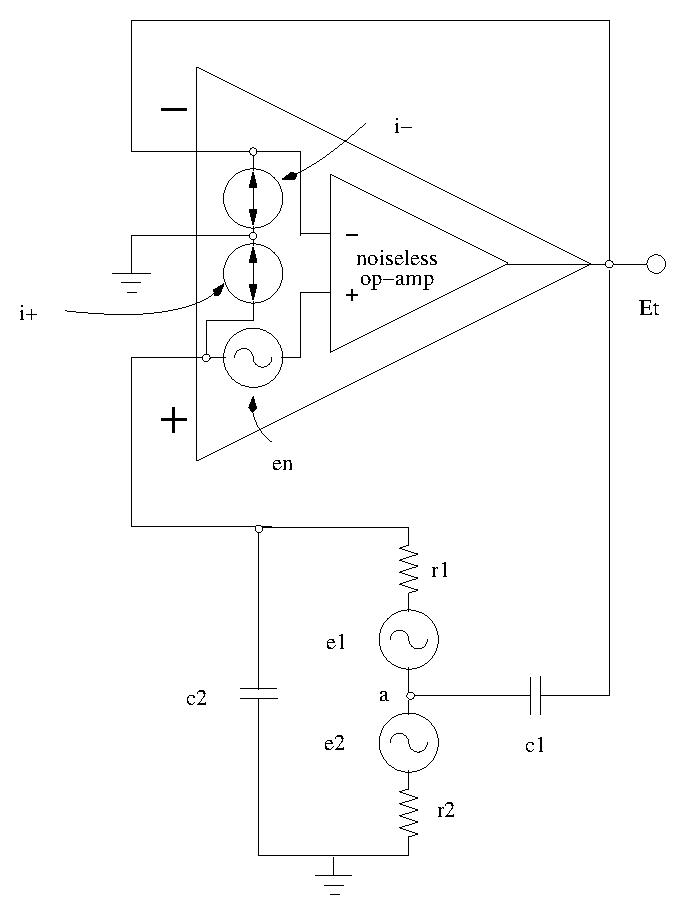
\includegraphics{ae-noise-eq.eps}
	\caption{Active electrode equivalent noise circuit.}
	\label{fig:ae-noise-eq}
	\end{center}
\end{figure}

Random noise sources in operational amplifiers are generally referred
to the amplifier input. The equivalent noisy amplifier are modeled as
a group of uncorrelated noise generators in series and parallel with
the inputs of a noiseless operational amplifier
\cite[11]{noise-analysis}. 

Figure~\vref{fig:ae-noise-eq} depicts the equivalent active electrode
noise circuit of Figure~\vref{fig:active-electrode}. In the equivalent
circuit the signal input is grounded and five noise sources are added:
\begin{itemize}
	\item A internal voltage noise source $\overline{e_{int}}$ referred
	to the non-inverting amplifier input.

	\item Two Johnston noise sources $\overline{e_{R_1}}$ and
	$\overline{e_{R_1}}$ contributed by $R_1$ and $R_2$.

	\item Two internal current noise sources $\overline{i_n}$ and
	$\overline{i_p}$ alternatively referred to the inverting and
	non-inverting amplifier inputs.

\end{itemize}

\subsubsection{Equivalent noise circuit analysis}
The principle of superposition may be applied due to the uncorrelated
nature of the individual noise sources. A single noise source is
isolated and all other sources ignored. By applying standard circuit
analysis techniques the system noise generated by a single source is
calculated. This procedure is followed for all noise sources and the
total noise value calculated by applying Equation~\ref{eq:noise-rms}.


The average value $\overline{E_{R_1}}$ is determined by disregarding
all noise sources except $R_1$ and summing the currents away from node
$a$ in Figure~\vref{fig:ae-noise-eq}:
\begin{equation}
	\overline{E_{R_1}} = \overline{e_1}(\frac{Z_1}{R_1 + Z_2} +
	\frac{Z_1}{R_2} + 1)
	\label{eq:noise-er1t}
\end{equation}
With $Z_1$ and $Z_2$ the impedances due to capacitors $C_1$ and $C_2$
respectively. To minimize the Johnston noise component the maximum
resistance used in the active electrode must be kept to a minimum,
that is $R_1$ = $R_2$ = $R$ as stated in
Section~\ref{section:comp-values}.
\begin{equation}
	\overline{E_{R_1}} = \overline{e_{R_1}}\left(\frac{Z_1(2R +
	Z_2)}{R(R + Z_2}) \right)
\end{equation}

Squaring the mean value $\overline{e_{R_1}}$ and substituting into the
thermal noise equation (Equation~\ref{eq:noise-thermal}) leads to the
system thermal noise due to $R_1$:
\begin{equation}
		\overline{E_{R_1}}^2 = \overline{e_{R_1}}^2\left (\frac{Z_1(2R +
	Z_2)}{R(R + Z_2)} \right )^2
\end{equation}

\begin{equation}
	\Rightarrow	\overline{E_{R_1}}^2 = 4kTR\int\/\left (\frac{Z_1(2R +
	Z_2)}{R(R + Z_2)} \right )^2df
	\label{eq:noise-therm1}
\end{equation}

Similar reasoning holds for $R_2$:
\begin{equation}
	\Rightarrow	\overline{E_{R_1}}^2 = 4kTR\int\/\left (\frac{Z_1(2R +
	Z_2)}{R(R + Z_2)} \right )^2df
	\label{eq:noise-therm2}
\end{equation}

From Equation~\ref{eq:noise-rms} follows that the total RMS noise
voltage due to the active electrode external resistors is the root sum
of Equations~\ref{eq:noise-therm1} and \ref{eq:noise-therm2}:
\begin{equation}
	E_{RMS} = \sqrt{\overline{E_{R1}^2} + \overline{E_{R_2}^2}}
	\label{eq:noise-rtot1}
\end{equation}
\begin{equation}
	\Rightarrow E_{RMS} = \sqrt{\int \left (8kTR
	\left(\frac{Z_1(2R + Z_1)}{R(R + Z_2)} + 1\right)^2 \right) df}
	\label{eq:noise-rtot2}
\end{equation}

The external resistors are the only devices that can be varied in the
circuit design. The other noise sources are inherent to the active
devices and cannot be manipulated short of choosing the device
according to its published noise specifications.

For this reason the lowest resistor values were chosen that a design
will allow. The TL071 ($v_n = 18~\frac{nV}{\sqrt{Hz}}$)\footnote{TL071
Data sheet} operational amplifier were chosen to implement all active
components of the system excluding the instrumentation amplifier.

\subsection{Physical electrode implementation}
\begin{center}
\begin{figure}[htbp]
	\begin{center}
	\psfrag{x1}{$x_1$}						
	\psfrag{x2}{$x_2$}						
	\psfrag{x3}{$x_3$}						
	\psfrag{x4}{$x_4$}						
	\psfrag{y1}{$y_1$}
	\psfrag{y2}{$y_2$}
	\psfrag{y3}{$y_3$}
	\psfrag{a}{a}
	\psfrag{b}{b}
	\psfrag{c}{c}
	\psfrag{d}{d}
	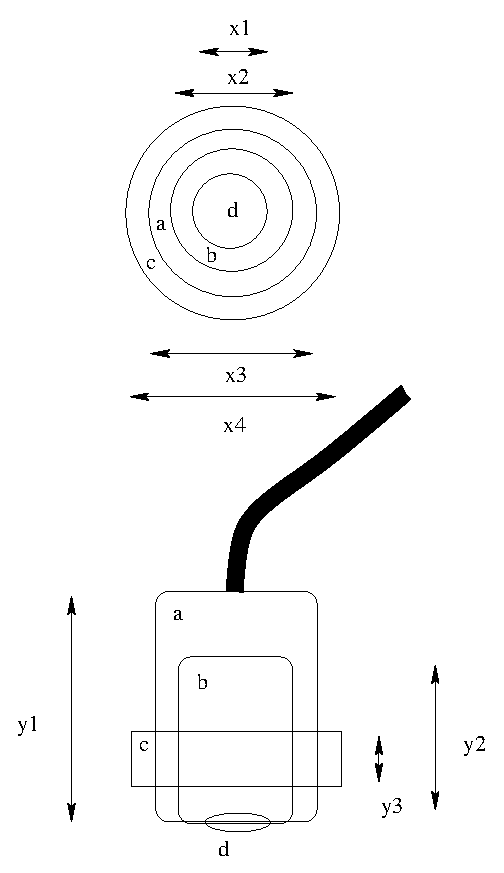
\includegraphics{electrode-imp.eps}
	\caption{Active electrode structural design parameters.}
	\label{fig:electrode-structure}
	\end{center}
\end{figure}
\end{center}

\begin{table}
\begin{center}	
	\begin{tabular}[htpb]{|c|c|} \hline
	Measurement & Value [mm] \\ \hline
	$x_1$ & 13 \\
	$x_2$ & 20 \\ 
	$x_3$ & 25 \\
	$x_4$ & 33 \\
	$y_1$ & 30 \\
	$y_2$ & 20 \\
	$y_3$ & 7 \\
	\hline
	\end{tabular}
	\caption{Active electrode dimensions}
	\label{table:ae-dim}
\end{center}	
\end{table}

Figure~\vref{fig:electrode-structure} depicts the active electrode as
a single physical unit. Table~\ref{table:ae-dim} lists the electrode
dimensions. Casings a,b and c are press--molded vulcanized rubber
plugs available commercially. The active electrode circuitry is
contained in plug b. The passive electrode (d) may be silver--plated
\footnote{The process of Ag--plating is outlined in
Appendix~\ref{appendix:plating} } to reduce contamination noise levels
\cite{electrode-stability}. 

Encapsulating the AE electronics in the electrode body allows for a
neat and manageable device. The encapsulating rubber also acts as a
robust cage, protecting the electronics against impact. The external
electrode housing surface were treated with Graphit\footnote{GRAPHIT,
Kontakt Chemie, CRC Industries, Belgium}, a graphite containing
surface paint. The surface paint aids in the prevention of possible
destructive static build--up on the electrode housing.


\begin{center}
\begin{figure}[htbp]
	\begin{center}
	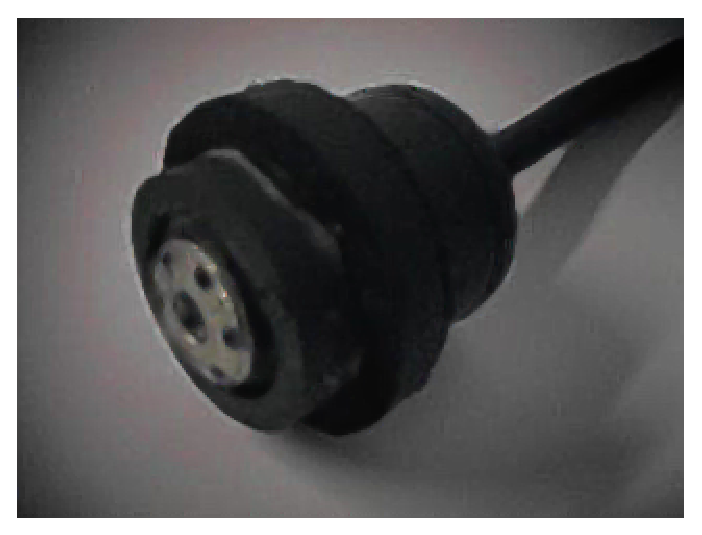
\includegraphics{electrode.ps}
	\caption{Active electrode implementation.}
	\label{fig:electrode-implimentation}
	\end{center}
\end{figure}
\end{center}

Figure~\ref{fig:electrode-implimentation} is a photograph of an active
electrode ('Blue')\footnote{The AE's were labeled 'Blue' and 'Red'}
used in the project. The outer and inner housing as well as the
mounting ring is visible. The inner plug containing the AE electronics
fits into the outer plug with the connecting cable threaded through
the base of the outer plug. The top of the inner plug supports the
passive electrode interface.

During active electrode implementation it was decided to use the
Ag/AgCl metal electrodes embedded in standard ECG gel electrodes as
active electrode tips. The passive electrode was replaced with a clip
that fits most standard ECG electrode fasteners. The clip is visible
at the front of the electrode in
Figure~\ref{fig:electrode-implimentation}.


\subsection{SAM container implementation}
\begin{figure}[htbp]
	\begin{center}
	\psfrag{wool}[][]{Velcro wool}
	\psfrag{hooks}[][]{Velcro hooks}
	\psfrag{x2}[][]{$x_2$}
	\psfrag{x1}[][]{$x_1$}		
	\psfrag{x3}[][]{$x_3$}		
	\psfrag{y1}[][]{$y_1$}
	\psfrag{y2}[][]{$y_2$}
	\psfrag{z}[][]{$z$}
	\psfrag{d}[][]{$d$}
	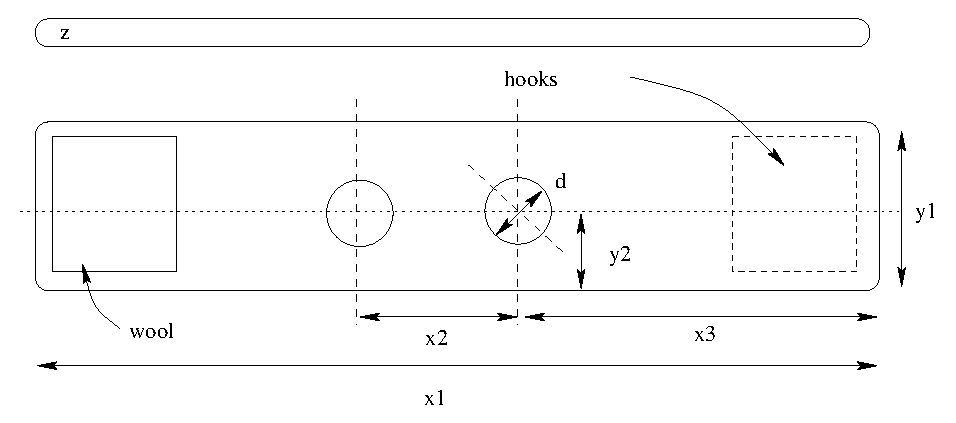
\includegraphics[width=\textwidth]{headband2.eps}
	\caption{SAM container implementation.}
	\label{fig:container}
	\end{center}
\end{figure}

\begin{table}
\begin{center}	
	\begin{tabular}[htpb]{|c|c|} \hline
	Measurement & Value [mm]\\ \hline
	$x_1$ & 670 \\ 
	$x_2$ & 90 \\
	$x_3$ & 280 \\
	$y_1$ & 50 \\ 
	$y_2$ & 25 \\ 
	$d$ & 23 \\ 
	$z$ & 4 \\
	\hline
	\end{tabular}
	\caption{SAM container dimensions}
	\label{table:sam-container}
\end{center}	
\end{table}

Figure~\vref{fig:container} details the SAM container
design. Table~\ref{table:sam-container} lists the SAM container
dimensions. The container resembles a sweat or head--band and is made
using a dense foam rubber strip and Velcro fasteners. The head--band
contains two holes that corresponds to the $F_{p1}$ and $F_{p2}$
montage positions when mounted. The diameter ($d$) of the holes are
slightly less than the diameter of the electrode outer plug, this
ensures a tight and secure fit of the electrode in the head--band.

\begin{center}
\begin{figure}[htbp]
	\begin{center}
	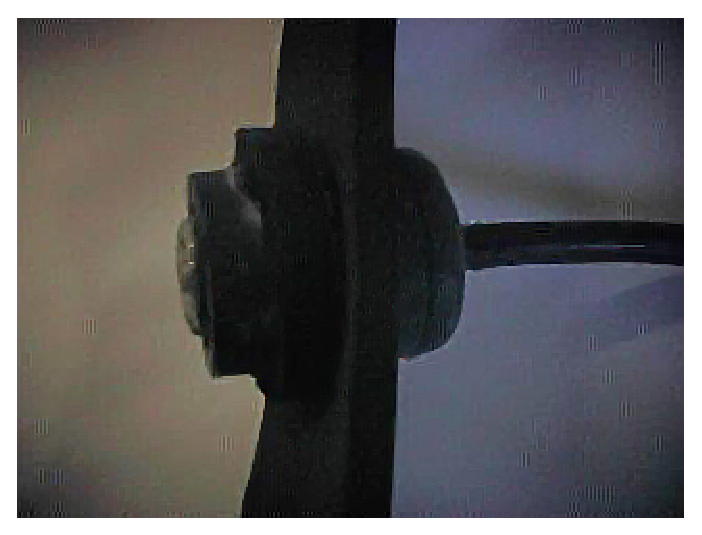
\includegraphics{single-electrode-headband.ps}
	\caption{Head--band mounted electrode.}
	\label{fig:headband-mounted-electrode}
	\end{center}
\end{figure}
\end{center}

Figure~\vref{fig:headband-mounted-electrode} shows an active electrode
mounted on the SAM head--band of Figure~\vref{fig:container}. The
outer plug fits snugly through the head--band hole.  When the
head--band is fastened on the head pressure is applied to the outer
ring and the electrode pressed against the skin. The applied pressure
from the head--band keeps the electrodes firmly in position at their
$F_{p1}$ and $F_{p2}$ positions.


\begin{center}
\begin{figure}[htbp]
	\begin{center}
	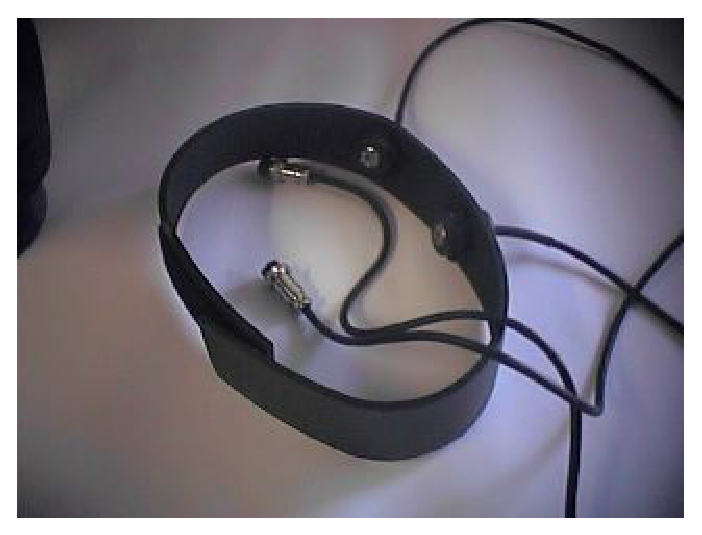
\includegraphics{electrode-headband.ps}
	\caption{Head--band mounted electrodes.}
	\label{fig:headband-mounted-electrodes}
	\end{center}
\end{figure}
\end{center}

Figure~\vref{fig:headband-mounted-electrodes} shows both electrodes
mounted in their respective positions. The head--band is positioned in
the same manner as when it is used during normal system operation. The
Electrode cable terminators are visible in the center of the
head--band circle.


\subsubsection{Electrode placement}
\begin{figure}[htbp]
\begin{center}
	\includegraphics*{electrodes-front-headband.ps}
	\caption{Electrodes mounted at $F_{p1}$ and $F_{p2}$}
\label{fig:mount1}
\end{center}
\end{figure}

The electrodes are positioned on the head--band in such a manner that
the electrode placement on the scalp will correspond to the $F_{p1}$
and $F_{p2}$ 10--20 EEG montage positions when the container is
fastened on the head, see Figure~\ref{fig:mount1}. The active
electrode clips are visible in front of the photograph. The Ag/AgCl
electrode tips are clipped unto the electrodes before use. 


\begin{figure}[htbp]
\begin{center}
	\includegraphics*{unmounted-SMEandSAM.ps}
	\caption{Unmounted SAM and SME}
	\label{fig:unSMEandSAM}
\end{center}
\end{figure}

Figure~\ref{fig:unSMEandSAM} shows the SAM container with the attached
electrodes together with the SME physical head module. The $F_{p1}$
and $F_{p2}$ on both the SAM and SME correspond.

\begin{figure}[htbp]
\begin{center}
	\includegraphics*{mounted-SMEanSAM.ps}
	\caption{Mounted SAM and SME}
	\label{fig:SMEandSAM}
\end{center}
\end{figure}

Figure~\ref{fig:SMEandSAM} shows the signal acquisition mounted on the
standard measurement environment head model. During noise and
interference measurements the SAM and SME modules were used in this
configuration. The test--setup of Figure~\ref{fig:SMEandSAM} was
physically moved closer and nearer suspected interference sources
during testing.

The configuration shown in Figure~\ref{fig:SMEandSAM} is the normal
manner in which the SAM is used when measurements on a human subject
is done.

\section{SAM measurements and characterization}

\subsection{Noise and interference measurements}

\begin{figure}[htbp]
\begin{center}
	\psfrag{+}[][]{+}
	\psfrag{-}[][]{-}
	\psfrag{TL071}[][]{TL071}
	\psfrag{s1}[][]{$S_1$}
	\psfrag{vo}[][]{$v_o$}
	\includegraphics*{ae-m.eps}
	\caption{AE noise measurement circuit}
	\label{fig:ae-m}
\end{center}
\end{figure}

Figure~\ref{fig:ae-m} represents the circuit used during the active
electrode noise measurements. Both AE used in the system were
evaluated. Measurements from each AE were very similar and no
distinction between either of the AE's were noticed or reported.
Measurements from only one AE are represented.

For noise measurements switch $S_1$ are either opened or closed. When
evaluating SME signals $S_1$ is always opened.

\begin{figure}[htbp]
\begin{center}
	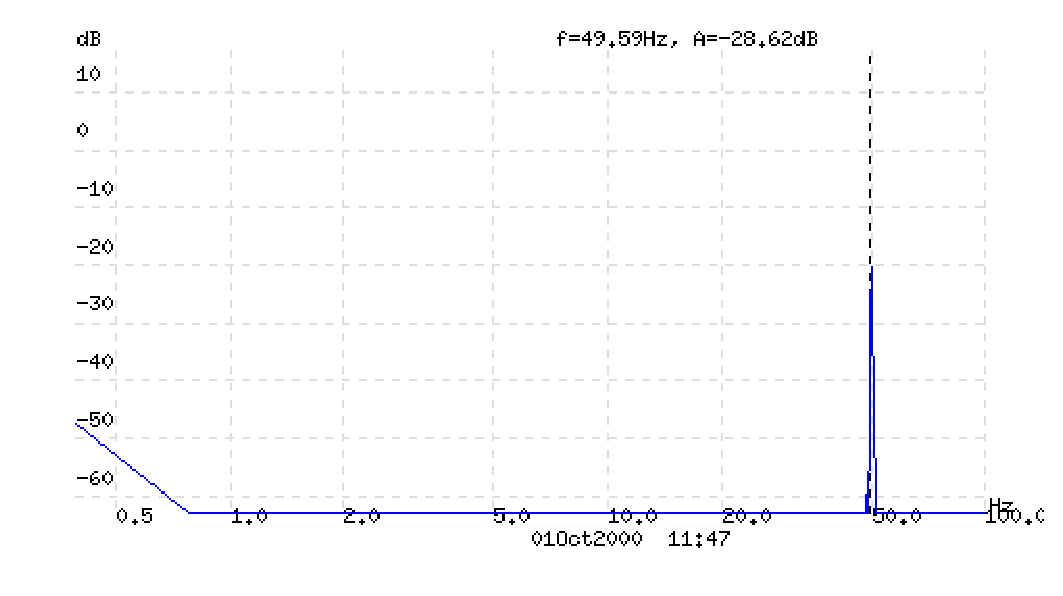
\includegraphics[width=\textwidth]{AE1OF.ps}
	\caption{AE off grounded}
	\label{fig:ae1-n}
\end{center}
\end{figure}
 
Figure~\ref{fig:ae1-n} represents the signal measured at the output of
the grounded ($S_1$ closed) un-powered active electrode. The noise
floor is nominally flat with the -28~dB 50~Hz interference spike the
only relevant feature of the graph. The measurement of
Figure~\ref{fig:ae1-n} and all other measurements note in this section
were done with the 'Blue' AE of
Figure~\ref{fig:electrode-implimentation}. Shielded commercial
oscilloscope probes were used during all measurements, a floating
probe always displayed a -64~dB 50~Hz interference signal, the signal
of Figure~\ref{fig:ae1-n} consists therefore primarily of the
interference coupled into the AE.


\begin{figure}[htbp]
\begin{center}
	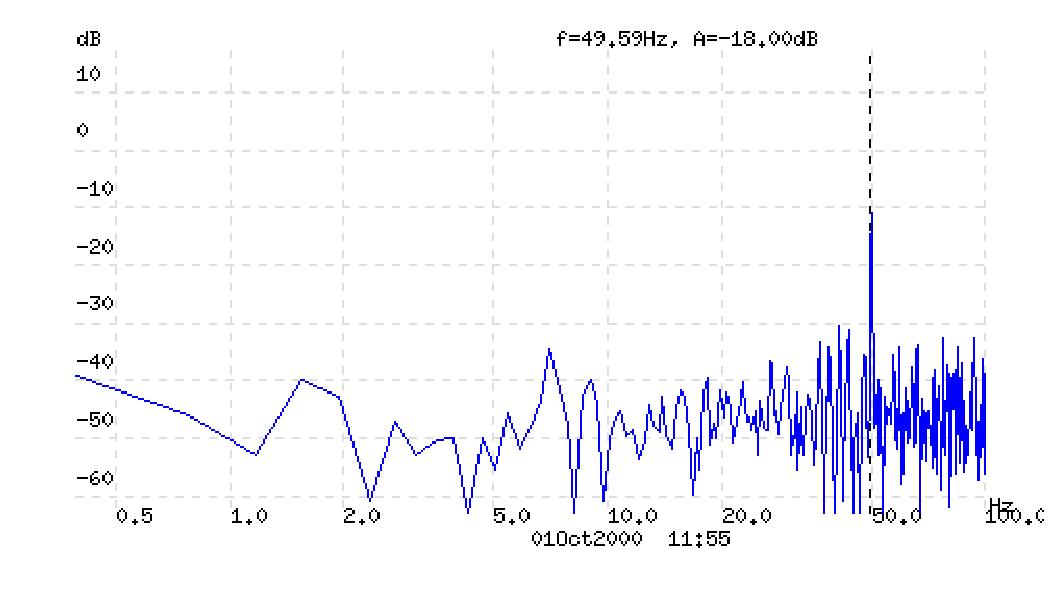
\includegraphics[width=\textwidth]{AE2OFOP.ps}
	\caption{AE off un-grounded}
	\label{fig:ae2-n}
\end{center}
\end{figure}

Figure~\ref{fig:ae2-n} represents the signal measured at the output of
the un-grounded ($S_1$ open) un-powered active electrode. The noise
floor is approximately -20~dB higher than that of
Figure~\ref{fig:ae1-n}. Once more a prominent feature of the graph is
the a -18~dB 50~Hz interference spike. Figure~\ref{fig:ae2-n}
represents the worse case noise scenario for a AE, input noise of this
magnitude will occur when the electrode loses contact with the
subject's skin.


\subsection{SME Measurements}
In order to test the frequency response of the AE the SME test signals
were applied to the AE input. The $100~\mu\/V$ signals from the SME
were to low to register on the test equipment and were raised for the
AE signal tests. Test signals of the magnitude used to test the AE
were very badly clipped even at the AD620 output. For system tests the
SME signals were adjusted to levels that were passed unclipped
throughout the system.


\begin{figure}[htbp]
\begin{center}
	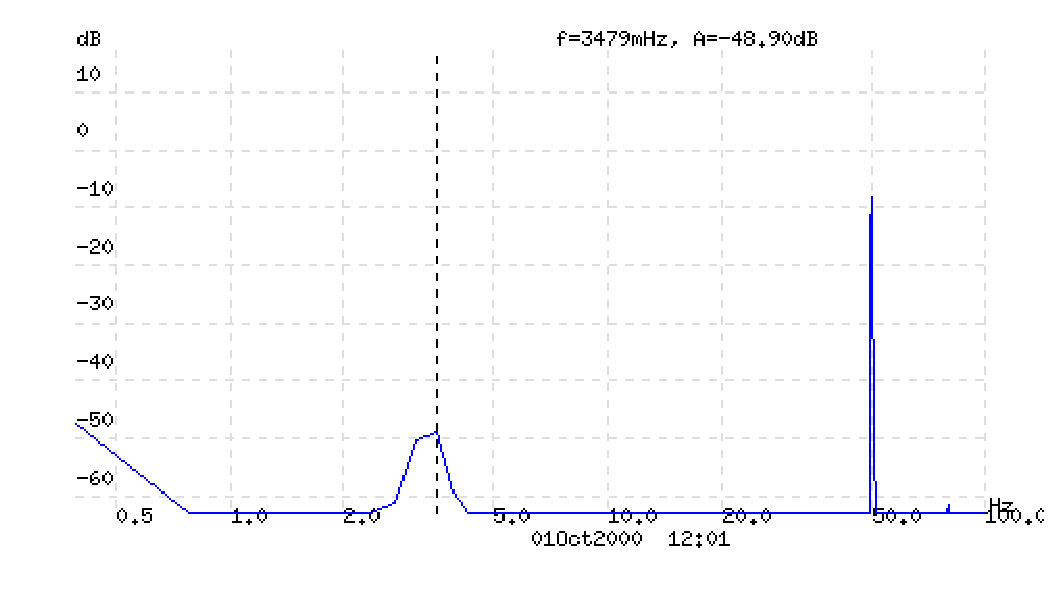
\includegraphics[width=\textwidth]{AE63SME.ps}
	\caption{$\delta$ (3~Hz) signal test}
	\label{fig:ae-sme3}
\end{center}
\end{figure}

Figure~\ref{fig:ae-sme3} represents the signal measured at the output
of the AE while applying a $\delta$ SME test signal at the SME
input. The $\delta$ signal amplitude were set at a visible value of
-50~dB (-48,9~dB measured). The 50~Hz interference signal is markedly
larger ($\pm$15~dB) than that of Figure~\ref{fig:ae1-n}. This is due
to the unshielded signal cables used to carry the test signal from the
SME to the AE.


\begin{figure}[htbp]
\begin{center}
	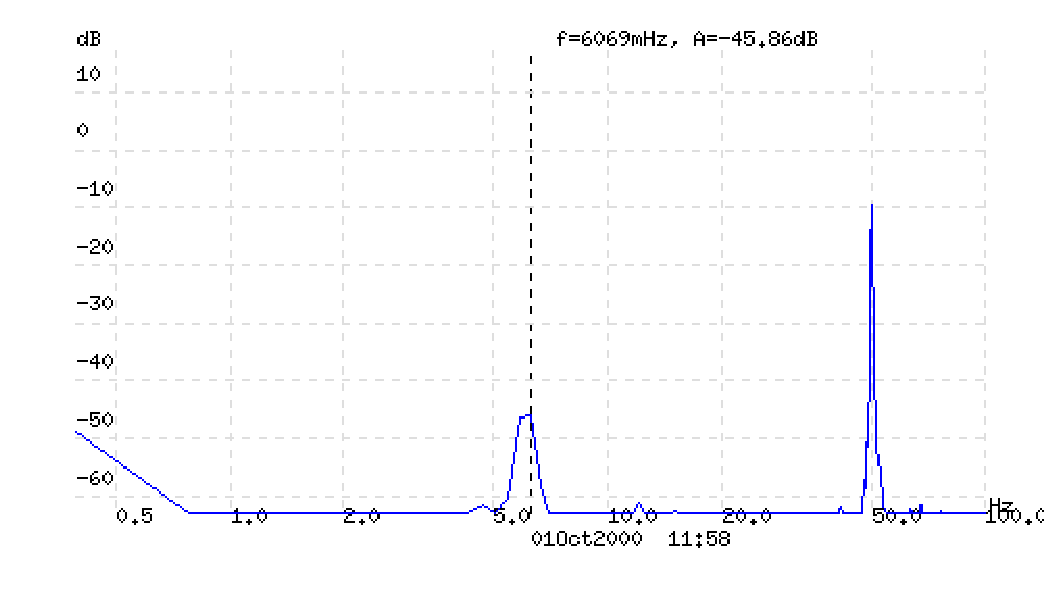
\includegraphics[width=\textwidth]{AE36SME.ps}
	\caption{$\theta$ (6~Hz) signal test}
	\label{fig:ae-sme6}
\end{center}
\end{figure}

Figure~\ref{fig:ae-sme6} represents the signal measured at the output
of the AE while applying a $\theta$ SME test signal at the SME
input. The $\theta$ signal amplitude were set at a visible value of
-50~dB (-45,86~dB measured). The mark at the 6~Hz spike were set
manually and is therefore not completely accurate.

\begin{figure}[htbp]
\begin{center}
	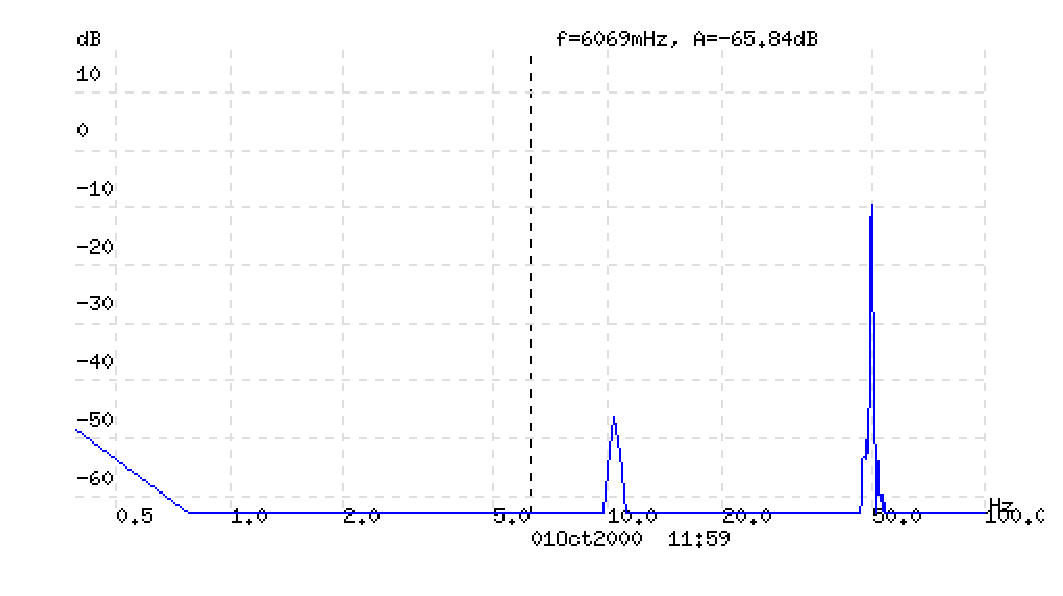
\includegraphics[width=\textwidth]{AE410SME.ps}
	\caption{$\alpha$ (10~Hz) signal test}
	\label{fig:ae-sme10}
\end{center}
\end{figure}

Figure~\ref{fig:ae-sme10} represents the signal measured at the output
of the AE while applying a $\alpha$ SME test signal at the SME
input. The $\alpha$ signal amplitude were set at a visible value of
-50~dB (-49,30~dB measured -- not visible on the graph). Various
points around the 10~Hz peak were tested for signal strength as the
$\alpha$~SME signal is used as the primary test signal during system
tests. The $\alpha$ SME signal has the lowest total harmonic
distortion in the SME test signal suite.


\begin{figure}[htbp]
\begin{center}
	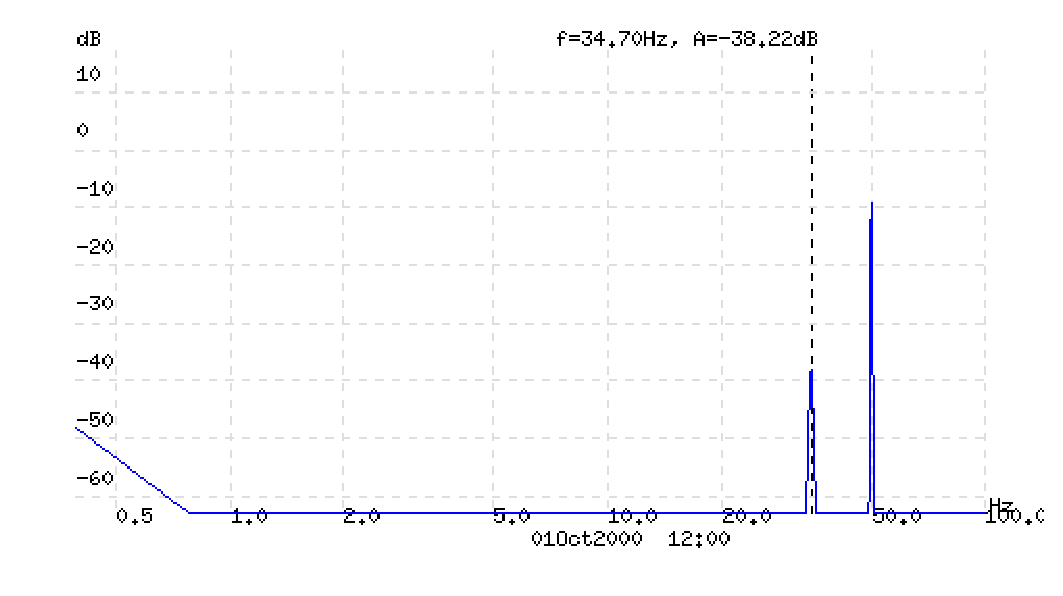
\includegraphics[width=\textwidth]{AE535SME.ps}
	\caption{$\gamma$ (35~Hz) signal test}
	\label{fig:ae-sme35}
\end{center}
\end{figure}

Figure~\ref{fig:ae-sme35} represents the signal measured at the output
of the AE while applying a $\gamma$ SME test signal at the SME
input. The $\gamma$ signal amplitude were set at a visible value of
-50~dB (-38,22~dB measured).

\subsubsection{Measurement conclusion}

The AE were evaluated using SME range of test frequencies. The AE did
not exhibit any unexpected behavior at any of the test
frequencies. The amount of 50~Hz interference present in the shielded
AE is higher than expected. Passive shielding of the AE cabling is not
as effective as was hoped. If time and effort permits a active shield
drive as described in the AD620 data sheet might be investigated.






\chapter{Low-level signal processing} \label{chap:llsp}
%copyright MJ Meintjes
%low level signal processing 
%included in skripsie.tex

\section{Overview}
The low-level signal processing module (LLSPM) extracts and amplifies
the EEG signal from the acquisition module output signal and reduces
the overall signal spectrum to the bandwidth of interest.

An instrumentation amplifier is deployed to isolate the differential
EEG signal from the common mode interference signal present at the
scalp surface. The cranial signal is applied to the instrumentation
amplifier inputs via the active electrodes described in
Chapter~\ref{chap:sa}. The resulting signal is band--limited by a set
of high and low--pass filters. Filtering the signal increases the
system signal to noise ratio by reducing the effective interference
bandwidth. The active and passive components in the filtering circuits
contributes to system noise levels lowering the SNR. Various
techniques and precautions are employed to reduce the filter and
differential stage system noise contributions.

DC components introduced by the instrumentation amplifier stage is
removed by applying a high-pass filter to the instrumentation
amplifier output. The high-pass filter output is amplified by a
variable amount before the signal is passed on to the next filter
stage.

A steep roll-off low-pass filter is employed to remove any signal
components above 50~Hz. A right-leg drive circuit is employed to
further minimize the common mode signal induced by power line and
fluorescent-light interference.


\section{LLSPM design specification}
The low-level signal processing module must be capable of extracting
and amplifying a 5~$\mu$V$_{pp}$ -- 100~$\mu$V$_{pp}$ signal from a
common mode signal several orders of magnitude larger. The resulting
differential signal must be amplified to within a -5~V~+~5~V range and
unwanted signal components removed. Care must be taken to reduce
signal noise and interference.

The LLSPM design specification is logically separated into a
differential signal extraction and a signal filtering submodule. The
design specification for each submodule is separately documented. The
convention of separately stating submodule specifications allows for
the substitution of any submodule with an alternative without adversely
affecting the overall system design. This keeps with the overall
modular tenet adhered to throughout the system design and
implementation process and may aid a process of comparative analysis
should such a requirement arise. The LLSPM must be housed in a small
EMI-resistant container and powered from the same battery pack as the
signal acquisition module.

\subsection{Differential amplifier design specification}
\label{section:dif-spec}
The differential amplifier stage of the LLSPM must reject common-mode
interference signals ($e_c$ Figure~\vref{fig:sme-eq}) and amplify the
differential EEG signal ($e_{EEG}$) as measured on the scalp
surface. In order to simplify design and increase signal quality a
commercial instrumentation amplifier device must be used. Because the
active electrodes employed in the signal acquisition module are AC
coupled (see Figure~\vref{fig:active-electrode}) the instrumentation
amplifier can be set close to its maximum gain setting without fear of
amplifier saturation or signal clipping. Setting gain close to maximum
enhances the CMRR and reduces the common mode interference
accordingly. The design must minimize the intrinsic system noise
contribution of the differential stage and component values must be
selected with cognizance of inherent component noise figures as noted
in Section~\vref{section:noise-analyses}. Table~\vref{table:df-specs}
summarizes the differential stage system parameters of the LLSPM
system specification.

\begin{table}
\begin{center}	
	\begin{tabular}[hpb]{|c|c|} \hline
	Parameter & Value \\ \hline
	Minimum CMRR & 100~dB \\
	Minimum Gain & 25~dB \\ 
	\hline
	\end{tabular}
	\caption{Differential amplifier specification}
	\label{table:df-specs}
\end{center}	
\end{table}



\subsection{Signal conditioning design specification}
\begin{figure}[htb]
\begin{center}
	\psfrag{G}[][]{$G$}
 	\psfrag{0db}[][]{0~dB} 
 	\psfrag{-3db}[][]{-3~dB} 
 	\psfrag{hpa}[][]{$A_{HPs}$} 
 	\psfrag{lpa}[][]{$A_{LPs}$} 
 	\psfrag{hps}[][]{$f_{HPs}$}
 	\psfrag{hpt}[][]{hp-trans} 
	\psfrag{fchp}[][]{$f_{HPc}$} 
	\psfrag{pb}[][]{Pass-band}
	\psfrag{f}[][]{f [Hz]}
	\psfrag{fclp}[][]{$f_{LPc}$}
	\psfrag{lpt}[][]{lp-trans}
	\psfrag{lps}[][]{$f_{LPs}$}
	\psfrag{rip}[][]{ripple}
	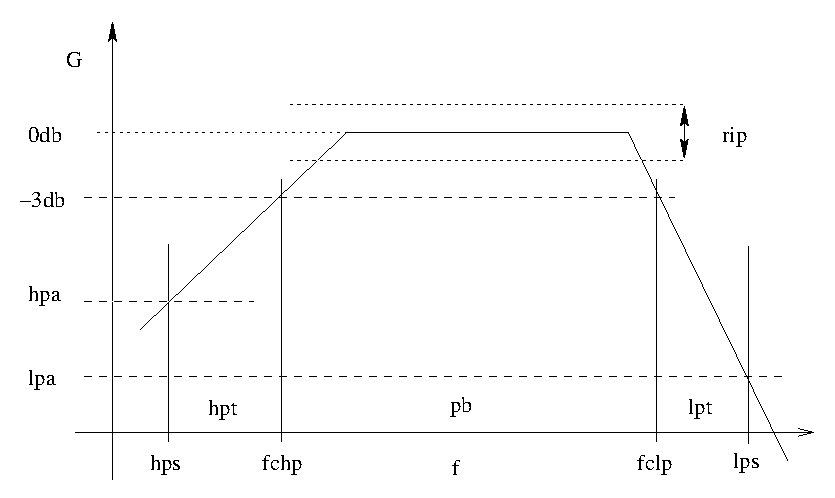
\includegraphics[width=\textwidth]{sig-cond-spec.eps}
	\caption{Signal conditioning specification}
	\label{fig:sig-cond-spec} 
\end{center}
\end{figure}

Figure~\vref{fig:sig-cond-spec} represents the frequency response
requirement for the signal conditioning submodule. The signal gain
($G$) is plotted against frequency from the high-pass filter stop
frequency $f_{HPs}$ to the low-pass filter stop frequency
$f_{LPs}$. The combination of the high-pass and low-pass filters acts
as a band-pass filter with the pass-band stretching from the high-pass
corner frequency $f_{HPc}$ to the low-pass corner frequency
$f_{LPc}$. The corner frequencies are chosen at the customary -3~dB or
half-power attenuation frequencies. Both filters have Butterworth
response characteristics as the $\pm$0.5~dB ripple budget is spent on
the active electrode response of Section~\ref{section:ae-imp}. The
amount of pass-band ripple contributed to the signal response must
therefore be 0~dB.

The slopes of the individual filters are determined by the attenuation
values $A_{HPs}$ and $A_{LPs}$ at the stop band frequencies $f_{HPs}$
and $f_{LPs}$. The slope specification determines the complexity of
the individual filters in number of pole
terms. Table~\vref{table:sc-specs} summarizes the chosen parameter
values indicated in Figure~\vref{fig:sig-cond-spec}.


\begin{table}
\begin{center}	
	\begin{tabular}[htpb]{|c|c|} \hline
	Parameter & Value \\ \hline
	$f_{HPs}$ & 0.05~Hz \\
	$f_{HPc}$ & 0.1~Hz \\ 
	$f_{LPc}$ & 35~Hz \\
	$f_{LPs}$ & 50~Hz \\
	$A_{HPs}$ & -40~dB \\
	$A_{LPs}$ & -50~dB \\
	\hline
	\end{tabular}
	\caption{Signal conditioning specification}
	\label{table:sc-specs}
\end{center}	
\end{table}

The high-pass corner frequency $f_{HPs}$ is chosen as 0.1~Hz in order
to include low $\delta$ frequency EEG signal information. Although
current EEG
research~\footnote{http://www.medizin.uni-tuebingen.de/medpsych/projekte/frequenc.htm}
suggests that human $\gamma$-band EEG activity is correlated with
abstract conceptualization, and does therefore contain relevant EEG
information, the low-pass filter is designed to attenuate all
frequencies above $f_{LPc}$. This decision simplifies system design
and implementation while retaining the bulk of EEG information used in
clinical practice for analysis and diagnosis.

The stop-band attenuation value for the low-pass filter $A_{LPs}$ is
dictated in part by the anti-aliasing requirements of the signal
conversion module of Chapter~\ref{chap:sc}. Because aliasing is a
fundamental mathematical result of the sampling process it is
preventable only by removing the frequency components above the
Nyquist frequency. For a signal undergoing A/D conversion the
amplitude of any frequency component above the Nyquist frequency
should at most influence only the least significant converter bit
\cite[p7]{design-guide}. Attenuation for frequencies above the Nyquist
frequency must be greater than 6$n$~dB with $n$ the bit resolution of
the converter. Because the EEG band is composed of low frequency
components (0.1~Hz~--~35~Hz) the sampling frequency can be set orders
of magnitude larger than $f_{LPc}$ negating most aliasing concerns.

The signal strength of the 50~Hz power line interference signal can be
significantly larger than that of the EEG signal
\cite{noise-rejection} \cite{fluorescent-interference}
\cite{fluorescent-interference2}, and must be effectively suppressed
to preserve signal quality and the system SNR.

\subsection{LLSPM container design specification}
In order to keep connecting signal wiring as short as possible both
the differential amplifier and signal conditioning submodules of the
LLSPM implementation must be situated physically near the SAM
container. To simplify construction and optimize space usage both
submodules will be contained in a single container. Grouping the
submodules together simplifies power and shielding requirements.


\section{LLSPM implementation}
\subsection{Differential Amplifier design and implementation}
\begin{figure}[htbp]
	\begin{center}
	\psfrag{vo}{$v_o$}
	\psfrag{r1}[][]{$R_1$} 
	\psfrag{r2}[][]{$R_2$} 
	\psfrag{r3}[][]{$R_3$} 
	\psfrag{r4}[][]{$R_4$} 
	\psfrag{r5}[][]{$R_5$} 
	\psfrag{r6}[][]{$R_6$} 
	\psfrag{r7}[][]{$R_7$} 
	\psfrag{c1}{$C_1$}
	\psfrag{c2}{$C_2$}
	\psfrag{+}{+}
	\psfrag{-}{--}
	\psfrag{1}{1}
	\psfrag{2}{2}
	\psfrag{3}{3}
	\psfrag{5}{5}
	\psfrag{8}{8}
	\psfrag{6}[][]{6}
	\psfrag{vae1}{$v_{AE_1}$}
	\psfrag{vae2}{$v_{AE_2}$}
	\psfrag{dr}{$drive$}
	\psfrag{AD620}{AD620}
	\psfrag{TL071}{071}
	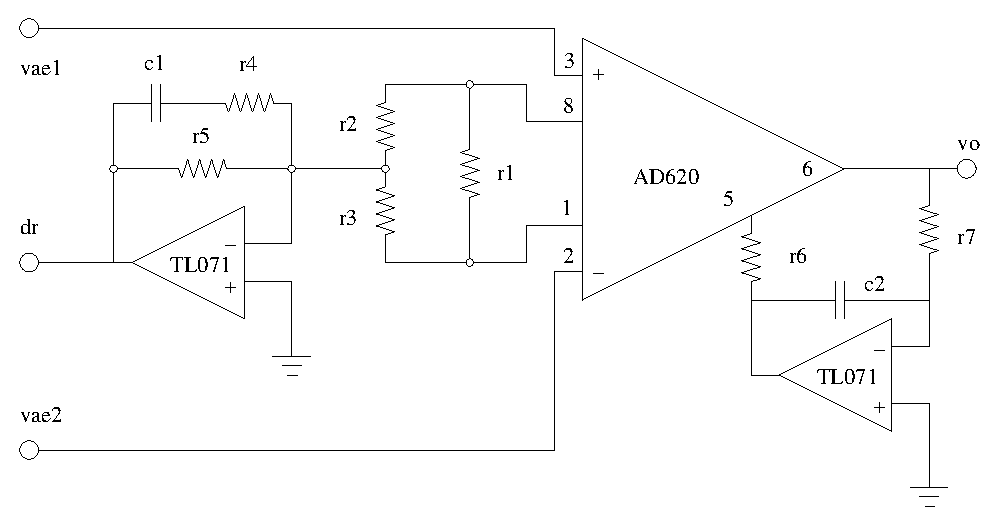
\includegraphics[width=\textwidth]{instrumentation-amp.eps}
	\caption{Differential amplifier implementation}
	\label{fig:instrumentation-amp} 
	\end{center}
\end{figure}

Figure~\vref{fig:instrumentation-amp} depicts the differential
amplifier sub-module deployed in the LLSPM. The differential stage is
implemented using the monolithic AD620 integrated instrumentation
amplifier available from Analog
Devices~\footnote{http://www.analog.com}. 

The AD620 consumes a maximum of 1.3~mA during normal operation making
it suitable for use in a battery operated system as specified in the
general LLSPM specification. The device has maximum nonlinearity of
40~parts per million, a maximum offset drift of
0.6~$\frac{\mu\/V}{^oC}$ and a maximum input offset value of
50~$\mu$V. The device has low input noise figures,
9~$\frac{nV}{\sqrt{Hz}}$ at 1~kHz, $\pm$0.28~$\mu\/V_{pp}$ in the
0.1~Hz~--~35~Hz band and 0.1~$\frac{pA}{\sqrt{Hz}}$ input current
noise~\footnote{AD620 data sheet}, which makes it suitable for use as
a pre-amplifier in the microvolt stages of a EEG signal amplitude
level (2~--~100~$\mu$V) data acquisition system.

The AD620 has a minimum CMRR of 110~dB ranging from DC to 60~Hz. This
performance specifications satisfies the differential amplifier design
specification noted in Section~\vref{section:dif-spec} and
Table~\ref{table:df-specs}.

\begin{table}
\begin{center}	
	\begin{tabular}[htpb]{|l|l|} \hline
	CMRR$_{min}$ (0 -- 60~Hz) & 110~dB \\
	Maximum Gain error ($\pm$10V) & 0.7\% \\
	$f_{-3~dB}$ & 12~kHz \\
	RTI (0.1~Hz -- 10~Hz) & 0.28~$\mu$V$_{p-p}$ \\
	\hline
	\end{tabular}
	\caption{AD620 specifications at $G = 500$}
	\label{table:ad620-1k}
\end{center}	
\end{table}
Table~\vref{table:ad620-1k} summarizes the relevant device
specifications as noted in the AD620 data sheet for a gain setting of
500.

The AD620's gain can be set accurately to within 0.15\% using a
single external gain resistor $R_g$. The gain resistance value is
calculated from the gain equation specified in the product data sheet:
\begin{equation}
	R_g = \frac{49.4~k\Omega}{G - 1}
	\label{eq:620-gain}
\end{equation}
With the device's gain set to $G = 500$, $R_g = 100~\Omega$. The gain
resistor $R_g$ is formed by the parallel $R_1$, $R_2$ and $R_3$
combination:
\begin{equation}
	R_g = \frac{R_1(R_1 + R_2)}{R_1 + R_2 + R_3}
	\label{eq:par}
\end{equation}
From Equation~\ref{eq:par} follows:
\begin{center}	
	\begin{tabular}[htpb]{|c|c|} \hline
	$R_1$ & 100~$\Omega$ \\
	$R_2$ & 100k~$\Omega$ \\
	$R_3$ & 100k~$\Omega$ \\
	\hline
	\end{tabular}
\end{center}	

The total resistance between pins 1 and 8 sets the AD620's gain value
to the value specified by Equation~\ref{eq:620-gain}. Where possible
1\% accurate metal film resistors where used.

\subsubsection{DC offset reduction}
The AD620 has a reference pin (5) from which can be used to set the
internal reference of the device. The output appearing at pin 6 is
referred to the voltage at pin 5. The DC--correcting circuit at the
AD620 output samples the output and feeds back a DC offset voltage to
the reference pin via the operational amplifier. This circuit
configuration reduces any DC offset voltages that may be present in
the output signal.

\begin{table}
\begin{center}	
	\begin{tabular}[htpb]{|l|l|} \hline
	$R_6$ & 10~k$\Omega$ \\
	$R_7$ & 1~M$\Omega$ \\
	$C_2$ & 300~nF \\
	\hline
	\end{tabular}
	\caption{AD620 reference pin driver}
	\label{table:dc}
\end{center}	
\end{table}

Table~\ref{table:dc} summarizes the component values of the reference
driver.

\subsubsection{Interference reduction}
The primary source of signal contamination in EEG acquisition systems
is environmental interference. The most prevalent sources of
interference are indoor power lines as well as fluorescent--light EMI
radiation. Power line interference is present as constant 50Hz signal
while the EMI radiated from the high--tension fluorescent--light coils
are present in the 1--10kHz range \cite{drive},
\cite{fluorescent-interference},
\cite{fluorescent-interference2}. These interference sources manifest
as large common mode voltage sources at the differential amplifier
inputs.

Due to non-linearities and component tolerances in the signal
acquisition paths the common mode voltage $v_c$ can be interpreted by
the instrumentation amplifier as a valid differential signal
\cite{drive}. 

In order to reduce $v_c$ a third electrode is used to provide a
low-impedance path between the subject and the amplifier
common. Directly connecting the electrode to the circuit ground is
undesirable for two reasons:
\begin{itemize}
	\item{A grounding electrode suffers from the same impedance
	problems as signal acquisition electrodes. A grounding electrode
	may represent up to 100k$\Omega$ between circuit ground and the
	subject's skin surface.}

	\item{Dangerous currents may flow through the grounding electrode
	if the patient should touch live power wiring. The threat of
	micro-shock is not as prevalent as in the case of ECG
	measurements, depending on the physical location of the grounding
	electrode, but may still lead to current burns.}
\end{itemize}

For these reasons the grounding electrode is usually driven by a
``right--leg drive circuit'' (RLD), named after the circuit's use in
ECG systems which uses a driven ground electrode attached to the
subjects right leg. The use of a driving circuit reduces the effective
electrode resistance by several orders of magnitude while allowing
only a save amount of current to flow through the grounding electrode.


\subsubsection{Right--leg drive design and implementation}

The reason for using a RLD circuit is to reduce $v_c$ to the lowest
possible level. Because of the exceptionally low voltage levels of EEG
signals (1--100~$\mu$V) a RLD needs to be optimally designed.

\subsubsection{Optimal Right--leg drive design}

The optimal RLD design was attempted according to a method by Winter
and Webster \cite{drive}.


\begin{figure}[htbp]
	\begin{center}
	\psfrag{i}[][]{100~nA}
	\psfrag{+}[][]{+}
	\psfrag{-}[][]{-}
	\psfrag{ad}[][]{$A_d$}
	\psfrag{ae}[][]{$A_e$}
	\psfrag{vo}[][]{$v_o$}
	\psfrag{vc}[][]{$v_c$}
	\psfrag{f}[][]{50~Hz}
	\psfrag{id}[][]{$i_d$}
	\psfrag{id1}[][]{$i_{d1}$}
	\psfrag{id2}[][]{$i_{d2}$}
	\psfrag{id3}[][]{$i_{d3}$}
	\psfrag{c1}[][]{$2~pF$}
	\psfrag{c2}[][]{$C_b$}
	\psfrag{re1}[][]{$R_{e1}$}
	\psfrag{ro}[][]{$R_o$}
	\psfrag{st}[][]{$S_1$}
	\psfrag{sg}[][]{$S_g$}
	\psfrag{rf}[][]{$R_f$}
	\psfrag{ra}[][]{$\frac{R_a}{2}$}
	\psfrag{c3}[][]{$2C_1$}
	\psfrag{c4}[][]{$C_s$}
	\psfrag{r1}[][]{$\frac{R_1}{2}$}
	\psfrag{re2}[][]{$\frac{R_{e2}}{2}$}
	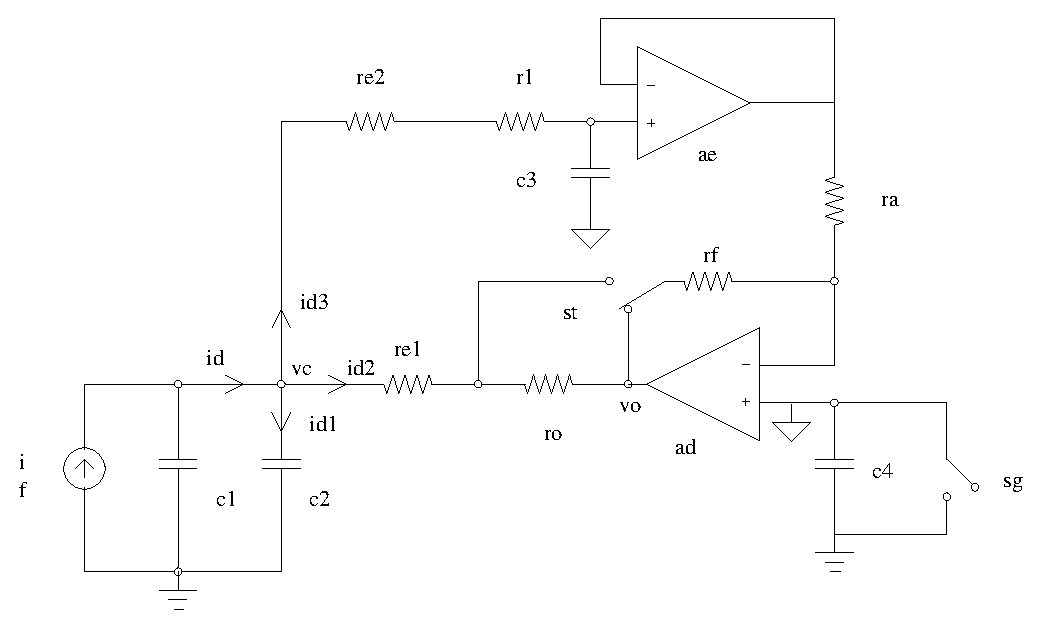
\includegraphics[width=\textwidth]{rld-opt1.eps}
	\caption{Right--leg drive equivalent circuit}
	\label{fig:rld-opt1} 
	\end{center}
\end{figure}


Figure~\vref{fig:rld-opt1} depicts the equivalent input side of the
differential input circuit of
Figure~\ref{fig:instrumentation-amp}. The averaging resistor
$\frac{R_a}{2}$ is equal to $\frac{R_2}{2}$ and $\frac{R_1}{2}$ of
Figure~\ref{fig:instrumentation-amp} ($R_1 = R_2 = 100~k\Omega$). The
electrode resistance $R_{e2}$ is the resistance introduced by the
stratum granulosum and is chosen as $100~k\Omega$. The low-pass filter
existing at the electrode input may be implemented in order to filter
out RF range frequencies. The RF interference could be demodulated by
the active electrodes into interference in the 0.1--35~Hz range. In
the implementation of the LLSPM these LP filters have been omitted as
they impair the effective CMRR of the amplifier at higher frequencies.

A low--pass filter due to parasitic capacitances between the cable
lead and common already exist at the input side of the operational
amplifier. The $R_1$ and $C_1$ values are lumped equivalents of a
implemented as well as the ever--present parasitic lead filter.

With the switch $S_g$ open the circuit of Figure~\ref{fig:rld-opt1}
represents an isolated amplifier with $C_s$ a stray capacitance to
environment ground. The capacitance between environment ground and the
subject is represented by $C_b$.

The object of a optimal RLD design is to calculate values for $R_o$
and $R_f$ for which the common mode voltage $v_c$ will be a minimum.


A displacement current $i_d$ flows between nearby power lines and the
body of the subject via stray capacitances. The capacitances are
lumped together as a 2~pF capacitor and exists in parallel with a
100~nA 50~Hz current source. The current $i_{d3}$ flowing into the
active electrode is assumed to be at least a order of magnitude
smaller that the $i_{d2}$ current flowing via the RLD to ground, that
is $i_{d3}~<<~i_{d2}$. The displacement current divides into $i_{d1}$
which flows directly to ground via $C_b$ and the $i_{d2}$ current
which flows to ground via the RLD circuit as follows:
\begin{equation}
	i_{d2} = \frac{i_dC_s}{C_s + C_b}
	\label{eq:id2}
\end{equation}

The gain ($G$) of the RLD amplifier $A_d$ is determined by $R_a$ and
$R_f$ with the normal inverting amplifier equation:
\begin{equation}
	G = \frac{2R_f}{R_a}
	\label{eq:G}
\end{equation}

From Equation~\ref{eq:G} follows the output voltage of $A_d$ ($v_o$):
\begin{equation}
	v_o = -Gv_c = v_c - (R_o + R_{e1})i_{d2}
	\label{eq:vo}
\end{equation}
With $R_{e1}$ the ground electrode resistance and $R_o$ the output
current limiting resistor.

From Equation~\ref{eq:G} and Equation~\ref{eq:vo} follows a expression
for $R_c$ the equivalent common mode resistance:
\begin{equation}
	R_c = \frac{R_o + R_{e1}}{G + 1}
	\label{eq:rc}
\end{equation}
From which follows that $v_c = R_ci_{d2}$.

If the ground electrode is directly connected to circuit ground
(common) the effective resistance between the subject and common is
$R_{e1}$, the electrode resistance. If the ground electrode is driven
by a RLD circuit like that of Figure~\ref{fig:rld-opt1} and $G >
\frac{R_o}{R_{e1}}$, the effective resistance is $R_c$, reducing the
common mode voltage $v_c$. The common mode voltage may also be reduced
by decreasing the isolation capacitance $C_s$ with respect to the body
capacitance $C_b$.


Good amplifier isolation is essential for subject or patient
safety. International respected standards
(NFPA)\footnote{http://www.nfpa.org/About\_NFPA/about\_nfpa.html}
require that less than 20~$\mu$A of current flow through any connecting
leads should the patient come in contact with power line voltage. This
includes the two sensing electrodes as well as the ground electrode.

If switch $S_g$ is closed somehow (common = environmental ground) the
design must ensure that at least 11~M$\Omega = (\frac{220V}{20\mu\/A})$
of impedance exists between all amplifier leads and ground. The output
resistance $R_o$ can be increased to limit current flowing through the
RLD circuit, it does however not ensure save current levels through
the sensing electrodes.

The isolation capacitance must be low enough to ensure that only the
allowed current flows should a power line voltage appear on the
amplifier: $C_s < \frac{20~\mu\/A}{(2\pi\/50)(220~V)} =
260~pF$\footnote{South--African conditions}. This means that isolated
amplifiers with $C_s < 260~pF$ do not require $R_o$ to reduce current
flow from external sources. The necessity of using $R_o$ to protect
against transient currents during startup or shutdown is doubtful as
current flow of up to 5~mA for a duration of less than 200~ms does not
seem to pose a micro-shock hazard \cite{drive}.

Should $R_o$ be included, the RLD circuit can be improved by switching
$S_1$ to the up position. The circuit will now measure the voltage at
the electrode in stead of $A_d$'s output. The ground electrode voltage
is now $-Gv_c$ and $R_c$ is independent of $R_o$: $R_c =
\frac{R_{e1}}{G + 1}$. For large gain ($G$) values $v_c$ is inversely
proportional to the gain. That is to minimize $v_c$ the gain must be
maximized.

The RLD maximum gain value is limited by the circuit's stability. For
the RLD to oscillate a $-180^o$ phase shift must be introduced
somewhere in the circuit. As the active electrodes have unity gain
they do not contribute much phase shift in the 0.1--35~Hz band of
interest. The RLD's $A_d$ amplifier does however introduce a pole at
$f = \frac{B}{G}$ with $B$ the gain-bandwidth product of $A_d$,
(3~MHz)\footnote{TL071 data-sheet} and $G = \frac{2R_f}{R_a}$.



\begin{figure}[htbp]
\begin{center}
	\psfrag{+}[][]{+}
	\psfrag{-}[][]{-}  
	\psfrag{s2}[][]{$S_2$} 
	\psfrag{vc1}[][]{$v_{c1}$}
	\psfrag{vc2}[][]{$v_{c2}$}  
	\psfrag{ad}[][]{$A_d$} 
	\psfrag{r1}[][]{$R_o + R_{e1}$}
	\psfrag{r2}[][]{$\frac{R_{e2} + R_1}{2}$}
	\psfrag{c1}[][]{$\frac{C_bC_s}{C_b + C_s}$}
	\psfrag{c2}[][]{$2C_1$}    
	\psfrag{ae1, ae2}[][]{$A_{e1}, A_{e2}$} 
	\psfrag{g1}{$\frac{G}{1 + \frac{G}{2\pi\/B}s}$}
	\psfrag{g2}{$\frac{G}{1 + \frac{1}{2\pi\/B}s}$}
	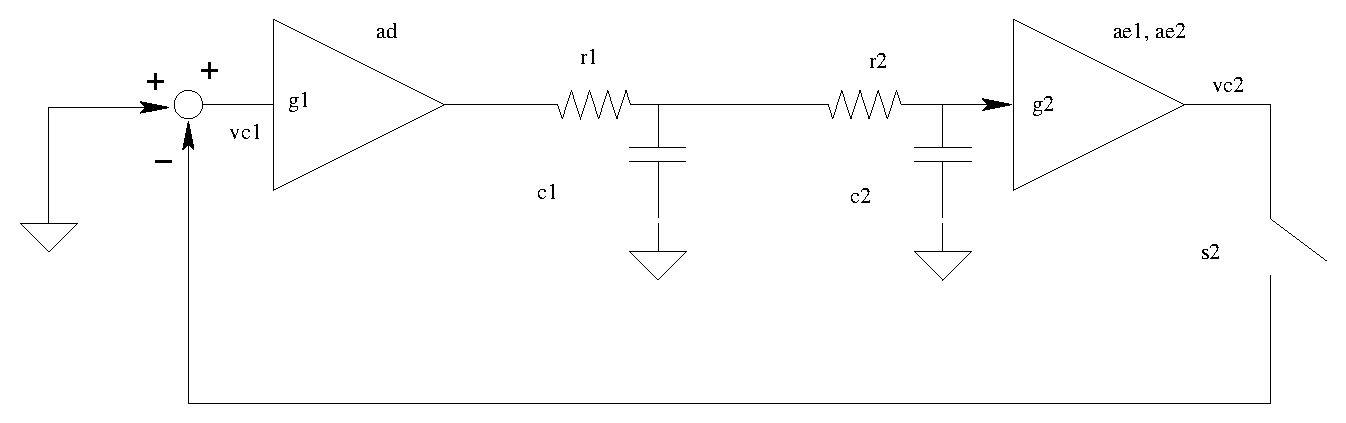
\includegraphics[width=\textwidth]{rld-gain.eps}
	\caption{Right-leg drive equivalent gain loop}
	\label{fig:rld-gain} 
\end{center}
\end{figure}

From Figure~\ref{fig:rld-gain} can be seen that two RC stages exist
which may introduce additional phase shifts in the RLD gain loop. The
first stage consist of the $R_o + R_{e1}$ series combination forming a
low pass filter with the $C_b + C_s$ combination. The other stage
consists of the $R_1 - C_1$ low pass filter discussed previously.

The low--frequency open--loop gain for the circuit depicted in
Figure~\ref{fig:rld-gain} is:


\begin{equation}
	\frac{v_{c1}}{v_{c2}} = \frac{G}{(1 + \frac{s}{2\pi\/f_a})(1 +
	\frac{ks}{2\pi\/f_n})(1 + \frac{s}{2\pi\/kf_n})}
	\label{eq:rld-gain}
\end{equation}

With $f_a$ the corner frequency of $A_d$ ($\frac{B}{G}$) and $B$ the
gain -- bandwidth product of $A_d$, and:
\begin{equation}
	G = \frac{2R_f}{R_a}
\end{equation}

\begin{equation}
	f_n = \frac{1}{2\pi\sqrt{\tau_1\tau_2}}
\end{equation}

\begin{equation}
	k = \zeta + \sqrt{\zeta^2 - 1}
\end{equation}

\begin{equation}
	\zeta = (\tau_1 + \tau_2 + \tau_3)\pi\/f_n
\end{equation}


The time constant for the first RC stage in Figure~\ref{fig:rld-gain}:
\begin{equation}
	\tau_1 = (R_o + R_{e1})\frac{C_bC_s}{C_b + C_s}
\end{equation}

The time constant for the second RC stage in Figure~\ref{fig:rld-gain}:
\begin{equation}
	\tau_2 = (R_{e2} + R_1)C_1
\end{equation}

The time constant $\tau_3$ relates how the second stage impedance loads
the first stage impedance:
\begin{equation}
	\tau_3 = 2(R_o + R_{e1})C_1
\end{equation}

If the loading effects of the second RC stage on the first RC stage
can be ignored, that is $\tau_3 << \tau_1$ or $\tau_3 << \tau_2$ then
Equation~\ref{eq:rld-gain} can be reduced to:
\begin{equation}
	\frac{v_{c2}}{v_{c1}} = \frac{G}{(1 + \frac{s}{2\pi\/f_a})(1 +
	s\tau_1)(1 + s\tau_2)}
\end{equation}

In order to keep the gain as high as possible while avoiding
oscillation the RLD is stabilized by using lag compensation. Lead
compensation is more difficult as the RLD circuit poles depend on
$R_{e1}$, $R_{e2}$ and $C_b$, which are variable depending on
environmental conditions.


In order to introduce lag compensation the corner frequency of the RLD
is lowered from $f_a$ to $f_{ac}$. The feedback impedance $R_f$ is can
be replaced with a capacitor $C_f$ as DC gain need not be limited.

The feedback capacitance in the RLD for the circuit in
Figure~\ref{fig:instrumentation-amp} is calculated using the following
values:
\begin{table}
\begin{center}	
	\begin{tabular}[htpb]{|c|c|} \hline
	$C_s$ & 200~pF \\
	$R_{e1}$, $R_{e2}$ & $1~\Omega$ \\
	$C_b$ & 200~pF \\
	$R_o$ & 10~k \\
	$C_1$ & 200~pF \\
	$R_1$ & 10~k \\
	\hline
	\end{tabular}
	\caption{RLD $C_f$ design values}
	\label{table:rld-cf}
\end{center}	
\end{table}

The values are chosen for a worse case scenario. From the above
follows that:

\begin{table}
\begin{center}	
	\begin{tabular}[htpb]{|c|c|} \hline
	$\tau_1$ & $1.001~\mu\/s$ \\
	$\tau_2$ & $2.002~\mu\/s$ \\
	$\tau_3$ & $4.004~\mu\/s$ \\
	$k$ & 4.7387 \\
	$f_n$ & 11.234~kHz \\
	\hline
	\end{tabular}
	\caption{RLD design constants}
	\label{table:rld-cfc}
\end{center}	
\end{table}

Seeing that the RC poles differ by more than a decade $f_ac$ must be
chosen in such a manner that the open loop gain of the RLD circuit has
at least a $45^o$ phase margin. With $f_{ac}$ the corner frequency of
$A_d$ with $C_f$ the capacitor in the feedback path:
\begin{equation}
	f_{ac} = \frac{1}{\pi\/G_oR_aC_f}
\end{equation}

With $f_L$ the lowest RC pole, that is:
\begin{equation}
	f_L = \frac{f_n}{k}
\end{equation}
And $G_o$ the low--frequency open loop gain of $A_d$:
\begin{equation}
	R_aC_f > \frac{k}{\pi\/f_n} = 134,2~\mu\/s
	\label{eq:rld-cf}
\end{equation}

\subsubsection{RLD bandwidth}
The gain of the RLD circuit at frequencies other than 50~Hz will
influence the reduction of interference at those frequencies. A large
contributer of high--frequency interference is fluorescent light
sources. Fluorescent light sources emit interference in the 1--10~kHz
range at a 100~Hz rate (2$f_l$, where $f_l$ is the power line
frequency, 50~Hz in South Africa). Parasitic low--pass filters at the
AD620 input may lower the CMRR for higher frequencies. For this reason
low pass filters were omitted from the IA front--end although they are
present in many commercial EEG systems. In order to reduce the
influence of high--frequency interference the bandwidth of the RLD must
include these interference frequencies.


\subsubsection{RLD realization}

\begin{figure}[htbp]
\begin{center}
	\psfrag{dr}[][]{$drive$}
	\psfrag{vc}[][]{$mv_c$}  
	\psfrag{r5}[][]{$R_5$} 
	\psfrag{r4}[][]{$R_4$} 
	\psfrag{ro}[][]{$R_o$} 
	\psfrag{c1}{$C_f$}
	\psfrag{+}{+}
	\psfrag{-}{--}
	\psfrag{TL071}{071}
	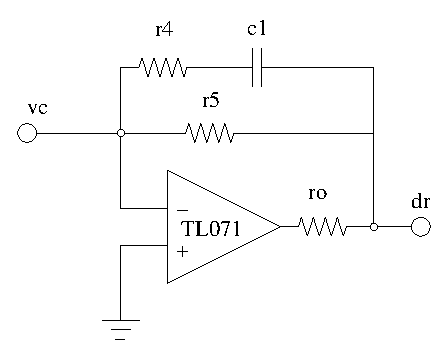
\includegraphics{rl-drive.eps}
	\caption{RLD drive circuit}
	\label{fig:rl-drive} 
\end{center}
\end{figure}


Figure~\vref{fig:rl-drive} represents the right-leg drive circuit of
Figure~\ref{fig:instrumentation-amp}. The circuit is realized using a
low-noise TL071 operational amplifier deployed as a inverting
integrating amplifier. The right-leg drive (RLD) circuit measures the
average of the common mode signal from the voltage tap created by the
$R_2$~--~$R_3$ voltage divider of
Figure~\vref{fig:instrumentation-amp}. The measured voltage is
inverted, amplified and fed back to the skin surface via the $drive$
electrode.

Non-optimal $v_c$ reducing RLD circuits seem to function as well or
within component error margins as that of optimally designed circuits
when used in ECG recording circuits \cite{drive}. However, for the
sensitive recording requirements of a EEG a optimally designed
right-leg drive is required to obtain the full noise suppression
capability potentially available from a optimally designed RLD. A
optimal circuit has the maximum gain allowed by the equations
governing the circuit's stability. 

The circuit bandwidth must allow for the inclusion and reduction of
fluorescent light interference frequencies. Circuit stability depends
on electrode resistance, RF interference and circuit decoupling
capacitance. The active electrodes described in Chapter~\ref{chap:sa}
reduces electrode resistance to less than 1~$\Omega$ and contributes
significantly to the stability of the RLD circuit \cite{drive}.


Component values were chosen as suggested by Equation~\ref{eq:rld-cf}
as well as the AD620 data sheet, $C_1$ is chosen to maintain stability
of the feedback loop.

\begin{table}
\begin{center}	
	\begin{tabular}[htpb]{|c|c|} \hline
	$R_4$ & 10~k$\Omega$ \\
	$R_5$ & 1~M$\Omega$ \\
	$C_f$ & 1~$\mu$F \\
	$R_o$ & $5~M\Omega$\\
	\hline
	\end{tabular}
	\caption{Right-leg drive component values}
	\label{table:rld}
\end{center}	
\end{table}

Table~\vref{table:rld} summarizes the component values used in the
right-leg drive circuit implementation.




\subsection{Signal Conditioning}
The differential amplifier output signal consists of the EEG
information in the band of interest (0.1~Hz~-~35~Hz), as well as
interference components above 35~Hz and DC components below
0.1~Hz. The undesirable signal components are removed by filtering the
differential signal through a set of active filters. Filtering
confines the signal bandwidth to the band of interest and enhances the
signal to noise ratio by reducing out of band noise. The resulting
signal is amplified and buffered to protect against possible loading
effects from subsequent system modules.

The active filters used in the LLSPM is implemented using standard
Sallen-Key filter architecture. This design is chosen for its
simplicity and low parts count \cite[p273]{art}. Care is taken to
compensate for the architecture's sensitivity to component variations
by using high-accuracy components where possible.


\subsection{Sallen-Key filter analysis}
\label{section:sk}
\begin{figure}[htbp]
	\psfrag{vi}{$v_i$}
	\psfrag{vo}{$v_o$}
	\psfrag{ve}{$v_e$}
	\psfrag{z1}{$Z_1$}
	\psfrag{z2}{$Z_2$}
	\psfrag{z3}{$Z_3$}
	\psfrag{z4}{$Z_4$}
	\psfrag{a}{$a$}
	\psfrag{b}{$b$}
	\psfrag{c}{$c$}
	\psfrag{r4}{$R_4$}
	\psfrag{r3}{$R_3$}
	\psfrag{+}{+}
	\psfrag{-}{--}
	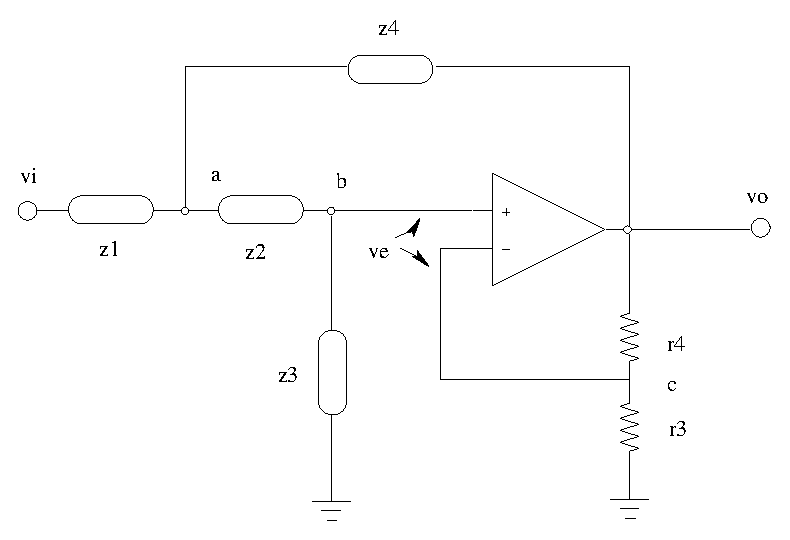
\includegraphics{sallen-key-gen.eps}
	\caption{Sallen-Key architecture.}
	\label{fig:sallen-key} 
\end{figure}

The operation of Sallen-Key filters are based on positive feedback
localized to the filter corner frequency $f_c$
\cite[p1]{sk-analysis}. Positive feedback enables the filter $Q$ to
be extended well above that of passive filters \cite[p267]{art}.

Figure~\vref{fig:sallen-key} depicts the general form of the
Sallen-Key architecture. $R_3$ and $R_4$ creates a non-inverting
voltage amplifier with frequency independent gain $K$. $Z_1$ to $Z_4$
dictates the frequency response characteristics of the filter. The
general 2-pole form of Figure~\vref{fig:sallen-key} is cascaded in
series to form more complex multi-pole filters with any of the
standard Butterworth, Chebyshev or Bessel responses. Each 2-pole
filter stage in a multi-pole filter represents a quadratic polynomial
factor of the $n$'th order polynomial describing the overall filter
transfer function \cite[p274]{art}.

\subsubsection{ Sallen-Key transfer function}
Determining the relationship between $v_i$, $v_o$, $v_b$ and $v_a$
allows the construction of a system gain-block diagram. Describing the
the system in this manner enables the formulation of a general
transfer function easily adopted to different filter configurations.

\begin{figure}[htbp]
	\psfrag{vo}{$v_o$}
	\psfrag{vi}{$v_i$}
	\psfrag{ve}{$v_e$}
	\psfrag{af}{$p(f)$}
	\psfrag{d}{$q$}
	\psfrag{b}{$r$}
	\psfrag{c}{$s$}
	\psfrag{+}[][]{+}
	\psfrag{-}[][]{--}
	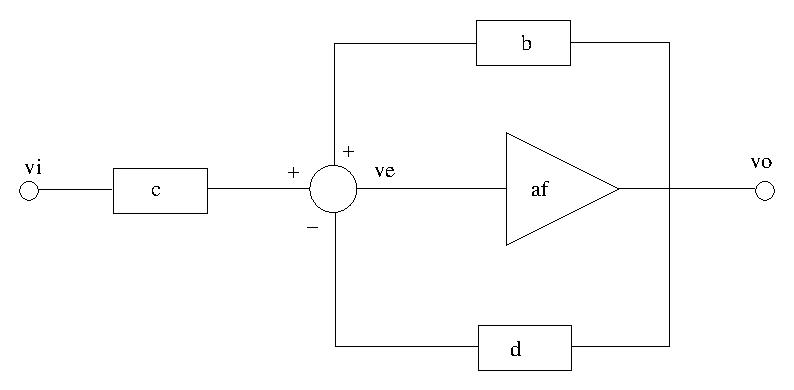
\includegraphics{sk-block.eps}
	\caption{Sallen-Key gain-block diagram.}
	\label{fig:sk-block} 
\end{figure}

Figure~\vref{fig:sk-block} represents the equivalent gain-block
diagram of the Sallen-Key filter described in
Figure~\vref{fig:sallen-key}. The gain values ($p$, $q$, $r$, $s$) in
Figure~\ref{fig:sallen-key} are determined by summing currents at
nodes $a$, $b$ and $c$ in Figure~\vref{fig:sk-block}. The relationship
between the node voltages are described in terms of the calculated
gain values in the feedback and forward-feed paths of the gain-block
diagram:
\begin{equation}
	v_e = sv_i + rv_o - qv_o	
	\label{eq:sk-t1}
\end{equation}
\begin{equation}
	v_o = p(f)v_i
	\label{eq:sk-t2}
\end{equation}
With $p(f)$ the open loop gain of the operational amplifier ($p(f) =
A_{open-loop}$). The frequency independent feedback gain $q$ through
$R_3$ and $R_4$ is that of the standard non-inverting operational
amplifier gain.
\begin{equation}
	q = \frac{R_3}{R_3 + R_4}
\end{equation}
The forward-feed gain of the input signal $v_i$ in terms of the $Z$
impedances.
\begin{equation}
	s = \frac{Z_2Z_3Z_4}{Z_2Z_3Z_4 + Z_1Z_2Z_4 + Z_2Z_3Z_1 + Z_2Z_2Z_4
	+ Z_2Z_2Z1}
\end{equation}
The feedback gain of the output signal $v_o$ in terms of the $Z$
impedances.
\begin{equation}
	s = \frac{Z_1Z_2Z_3}{Z_2Z_3Z_4 + Z_1Z_2Z_4 + Z_2Z_3Z_1 + Z_2Z_2Z_4
	+ Z_2Z_2Z1}
\end{equation}
Describing the circuit of Figure~\vref{fig:sallen-key} in voltage gain
terms simplifies the adaption of the general circuit transfer function
to either low or high-pass behavior. From Figure~\ref{fig:sallen-key}
and Equations~\ref{eq:sk-t1} and \ref{eq:sk-t2} the general Sallen-Key
filter transfer function is described as follows:
\begin{equation}
	\frac{v_o}{v_i} = \frac{s}{q}\left( \frac{1}{1 + \frac{1}{p(f)q}
	-\frac{r}{q}}\right ) 
	\label{eq:sk-trans}
\end{equation}
For a idealized operational amplifier the open loop gain
$p(f)~\rightarrow~\infty$ or
$\frac{1}{p(f)}~\rightarrow~0$. Substituting the impedance terms into
the idealized Equation~\ref{eq:sk-trans} leads to the general
Sallen-Key filter transfer function:
\begin{equation}
\frac{v_o}{v_i} = \frac{K}{\frac{Z_1Z_2}{Z_3Z_4} + \frac{Z_1}{Z_3} +
\frac{Z_1(1 - K)}{Z_4} + 1}
	\label{eq:sk-gen-tans}
\end{equation}
With $K = \frac{1}{q} = \frac{R_3}{R_3 + R_4}$, the frequency
independent feedback gain.

\subsection{High--pass filter design and implementation}
The resulting differential signal from the instrumentation amplifier
output may have a small DC offset voltage due to gain differences and
bias currents in the differential input buffer stages. The offset
voltage is normally very low due to the monolithic nature of the
instrumentation amplifier.

\begin{figure}[htbp]
	\psfrag{vo}{$v_o$}
	\psfrag{vi}{$v_i$}
	\psfrag{r1}[][]{$R_1$} 
	\psfrag{r2}[][]{$R_2$} 
	\psfrag{r3}[][]{$R_3$} 
	\psfrag{r4}[][]{$R_4$} 
	\psfrag{c2}[][]{$C_2$} 
	\psfrag{c1}{$C_1$}
	\psfrag{+}{+}
	\psfrag{-}{--}
	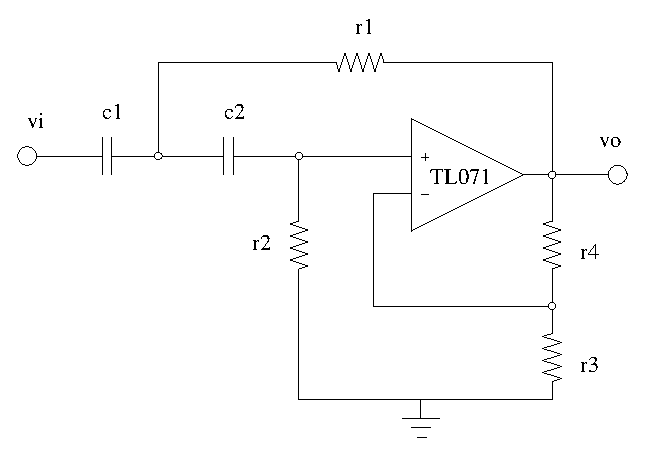
\includegraphics{high-pass.eps}
	\caption{Sallen-Key two-pole high-pass filter}
	\label{fig:high-pass} 
\end{figure}

The high pass-filter is implemented using the Sallen-Key architecture
described in Section~\vref{section:sk} with the $Z$ impedances adopted
for a high-pass filter response. Figure~\vref{fig:high-pass}
represents the circuit diagram for a Sallen-Key high-pass filter.

With $K = 1 + \frac{R_4}{R_3}$, $Z_3 = R_2$, $Z_4 = R_1$, $Z_2 =
\frac{1}{sC_2}$ and $Z_1 = \frac{1}{sC_1}$ the general transfer
function of Equation~\ref{eq:sk-trans} becomes:
\begin{equation}
	H(s)_{hp} = \frac{K(s^2R_1R_2C_1C_2)}{s^2(R_1R_2C_1C_2) + s(R_2C_2
	+ R_2C_1 + R_1C_2(1 - K) + 1)}
	\label{eq:lp-t1}
\end{equation}
Equation~\ref{eq:lp-t1} is significantly simplified by setting the
filter components as equal, $R_1 = R_2 = R$ and $C_1 = C_2 =
C$. Equating component values in this manner reduces system component
diversity and simplifies filter construction.
\begin{equation}
	H(s)_{hp} = \frac{Ks^2(RC)^2}{(RC)^2s^2 + s(2RC + RC(1 - K) + 1)}
	\label{eq:simp-hp}
\end{equation}
The filter design equations are reduced to simple relationships
describing the filter's $Q$ and corner frequency $f_c$.
\begin{equation}
	f_c = \frac{1}{2\pi\/RC}
	\label{eq:hp-fc}
\end{equation}

\begin{equation}
	Q = \frac{1}{3 - K}
	\label{eq:hp-q}
\end{equation}

Equation~\ref{eq:hp-q} illustrates the circuit's $Q$ dependence on the
gain value $K$ only, a additional gain stage must be used to achieve
the desired signal amplification. Because $f_c$ and $Q$ are
independent the filter transfer function can be manipulated to
represent any of the standard filter types. The high-pass filter
functions as expected in the low frequency (0.1~Hz--35~Hz) EEG
bandwidth. The filter has a upper cutoff frequency determined by the
open loop response of the operational amplifier. The TL071 device has
a low--pass cutoff of approximately 100~kHz.

The filter's departure from the ideal transfer function described in
Equation~\ref{eq:simp-hp} does not influence the EEG signal within the
bandwidth of interest.

\subsubsection{High-pass filter implementation}
A single two-pole filter stage is used in the high-pass filter
implementation. In order to preserve the flatness of the response
obtained from the active electrode described in Chapter~\vref{chap:sa}
a Butterworth response is chosen.

From \cite[p274]{art} Table~5.2 the gain $K$ is chosen as 1.586,
applying Equation~\ref{eq:hp-q} results in a $Q$ factor of
0.707. Choosing $C_1 = C_2$~=~2$\mu$F and applying
Equation~\ref{eq:hp-fc} results in $R_1 = R_2$~=~800~k$\Omega$. For
$R_4$~=~10~k$\Omega$, $R_3$ results in 17~k$\Omega$.


\begin{table}
\begin{center}	
	\begin{tabular}[htpb]{|c|c|c|c|} \hline
	Component & Value \\ \hline
	$C_1 = C_2$ & 2~$\mu$F \\
	$R_1 = R_2$ & 800~k$\Omega$ \\ 
	$R_4$ & 10~k$\Omega$ \\
	$R_3$ & 17~k$\Omega$ \\
	\hline
	\end{tabular}
	\caption{High-pass filter component values}
	\label{table:hp-comp}
\end{center}	
\end{table}
Table~\vref{table:hp-comp} is a summary of the component values used in
the high-pass filter implementation. Polyethylene capacitors and 1\%
accurate metal film resistors are used.


\subsection{Low--pass filter design and implementation}
\begin{figure}[htbp]
	\psfrag{vi}[][]{$v_i$} 
	\psfrag{vo}[][]{$v_o$}
	\psfrag{r1}[][]{$R_1$} 
	\psfrag{r2}[][]{$R_2$}
	\psfrag{r3}[][]{$R_3$} 
	\psfrag{r4}[][]{$R_4$} 
	\psfrag{c1}[][]{$C_1$}
	\psfrag{c2}[][]{$C_2$} 
	\psfrag{+}[][]{+} 
	\psfrag{-}[][]{--} 
	\includegraphics{low-pass.eps} 
	\caption{Sallen-Key two-pole low-pass filter.}  
	\label{fig:low-pass}
\end{figure}

The low-pass filter used in the signal conditioning sub-module is
required to reduce all signal components at 50~Hz to a minimum of
-72~dB. The strongest interference component attributed to power line
induction is encountered at 50~Hz and harmonics thereof. The roll-off
of the filter response from pass-band (35~Hz) to stop-band (50~Hz) is
steep and requires a fairly complex filter.

The low-pass filter is implemented using the Sallen-Key architecture
described in Section~\vref{section:sk} with the $Z$ impedances adapted
for a low-pass filter response. Figure~\vref{fig:low-pass} represents
the circuit diagram for a two-pole Sallen-Key low-pass filter.

With $K = 1 + \frac{R_4}{R_3}$, $Z_1 = R_1$, $Z_2 = R_2$, $Z_3 =
\frac{1}{sC_1}$ and $Z_4 = \frac{1}{sC_2}$ the general transfer
function of Equation~\ref{eq:sk-trans} becomes:
\begin{equation}
	H(s)_lp = \frac{K}{s^2(R_1R_2C_1C_2) + s(R_1C_2 + R_2C_2 +
	R_1C_1(1 - K) + 1)}
	\label{eq:hs-lp}
\end{equation}
Equation~\ref{eq:hs-lp} is significantly simplified by equating the
filter passive component values. By letting $C_1 = C_2 = C$ and $R_1 =
R_2 = R$ the filter's component diversity is reduced and the
implementation significantly simplified.
\begin{equation}
	H(s)_lp = \frac{1}{(RC)^2s^2 + s(2RC + RC(1 - K) + 1)}
	\label{eq:hs-lp2}
\end{equation}
The filter design equations are once more reduced to simple
relationships describing the filter's $Q$ and corner frequency
$f_c$. These relationships are identical to those describing the
high-pass filter's gain $K$ and quality factor $Q$ relationship, as
well ass the corner frequency $f_c$.
\begin{equation}
	f_c = \frac{1}{2\pi\/RC}
	\label{eq:lp-fc}
\end{equation}

\begin{equation}
	Q = \frac{1}{3 - K}
	\label{eq:lp-q}
\end{equation}

$f_c$ and $Q$ are independent the filter transfer function can be
manipulated to represent any of the standard filter types. The
low-pass filter functions as expected in the low frequency
(0.1~Hz--35~Hz) EEG bandwidth. For very high frequencies into the stop
band the filter acts as a high-pass filter due to non-linearities in
the open-loop output impedance. This departure from the ideal transfer
function does not influence the filter action in the band of interest.

\subsubsection{Low-pass filter implementation}
Multiple two-pole stage low-pass filters are cascaded in series to
obtain the necessary roll-off from the pass-band to the stop-band as
prescribed in the LLSPM specification in
Figure~\vref{fig:sig-cond-spec}. The filter is designed with a
Butterworth response in order to preserve the flatness of the total
system response. Choosing the a Butterworth response for the low-pass
filter in order to preserve flatness increases system complexity in
terms of component usage as well as system noise.

For the specified low-pass filter corner frequency $f_c = 35$~Hz and a
chosen capacitor value $C_1 = C_2 = 2\mu$~F, Equation~\ref{eq:lp-fc}
results in $R_1 = R_2 = 2.273$~k$\Omega$. From Table~5.2
\cite[p274]{art} the gain values $K$ for a ten-pole Butterworth filter
is chosen as specified per pole-pair. A two-pole set in series with a
eight-pole set is chosen and implemented as a single two-pole low-pass
Butterworth filter. The gain values are chosen for maximal gain in the
early stages in order to minimize noise amplification in the latter
filter stages.

The frequency-independent feedback loop formed by $R_4$ and $R_3$ gain
resistors are specified by the $R_4 = (K - 1)R_3$ relationship. The
filter is implemented using the low noise ($V_n =
18~\frac{nV}{\sqrt{Hz}}$) TL071 operational amplifier from Texas
Instruments, low-noise 1\% metal film resistors and low-drift
polypropylene capacitors.

\begin{figure}[htbp]
	\psfrag{TL071}[][]{071} 
	\psfrag{1}[][]{1} 
	\psfrag{2}[][]{2} 
	\psfrag{3}[][]{3} 
	\psfrag{4}[][]{4} 
	\psfrag{5}[][]{5} 
	\psfrag{vi}[][]{$v_i$} 
	\psfrag{vo}[][]{$v_o$}
	\psfrag{r1}[][]{$R_1$} 
	\psfrag{r2}[][]{$R_2$}
	\psfrag{r3}[][]{$R_3$} 
	\psfrag{r4}[][]{$R_4$} 
	\psfrag{r5}[][]{$R_5$} 
	\psfrag{r6}[][]{$R_6$} 
	\psfrag{r7}[][]{$R_7$} 
	\psfrag{r8}[][]{$R_8$} 
	\psfrag{r9}[][]{$R_9$} 
	\psfrag{r10}[][]{$R_{10}$} 
	\psfrag{r11}[][]{$R_{11}$} 
	\psfrag{r12}[][]{$R_{12}$} 
	\psfrag{c13}[][]{$C_{13}$}
	\psfrag{c14}[][]{$C_{14}$}
	\psfrag{c2}[][]{$C_2$} 
	\psfrag{c1}[][]{$C_1$} 
	\psfrag{+}[][]{+} 
	\psfrag{-}[][]{--} 
	\includegraphics[width=\textwidth]{lp-imp.eps} 
	\caption{Ten-pole low-pass filter.}  
	\label{fig:lp-imp}
\end{figure}

Figure~\vref{fig:lp-imp} depicts the low-pass filter used in the
LLSPM. 

\begin{table}
\begin{center}	
	\begin{tabular}[htpb]{|c|c|l|l|} \hline
	Stage & Gain & Component & Value \\ \hline
	1& 1.586 & $C_1 = C_2$ & 2~$\mu$F \\
	 & 		 & $R_1 = R_2$ & 2.273~k$\Omega$ \\ 
	 &		 & $R_3$ & 10~k$\Omega$ \\
	 &       & $R_4$ & 5.8~k$\Omega$ \\
	2& 2.610 & $C_1 = C_2$ & 2~$\mu$F \\
	 & 		 & $R_1 = R_2$ & 2.273~k$\Omega$ \\ 
	 & 		 & $R_5$ & 10~k$\Omega$ \\
	 & 		 & $R_6$ & 16.1~k$\Omega$ \\
	3& 1.889 & $C_1 = C_2$ & 2~$\mu$F \\
	 & 		 & $R_1 = R_2$ & 2.273~k$\Omega$ \\ 
	 & 		 & $R_7$ & 10~k$\Omega$ \\
	 & 		 & $R_8$ & 8.9~k$\Omega$ \\
	4& 1.337 & $C_1 = C_2$ & 2~$\mu$F \\
	 &    	 & $R_1 = R_2$ & 2.273~k$\Omega$ \\ 
	 & 		 & $R_{9}$ & 10~k$\Omega$ \\
	 &  	 & $R_{10}$ & 3.4~k$\Omega$ \\
	5& 1.038 & $C_1 = C_2$ & 2~$\mu$F \\
	 &  	 & $R_1 = R_2$ & 2.273~k$\Omega$ \\ 
	 & 		 & $R_{11}$ & 100~k$\Omega$ \\
	 &   	 & $R_{12}$ & 3.8~k$\Omega$ \\
	\hline
	\end{tabular}
	\caption{Low-pass filter component values}
	\label{table:lp-filter}
\end{center}	
\end{table}

Table~\vref{table:lp-filter} summarizes the component values used in
the low-pass filter realization.


\subsection{LLSPM Amplifier design and implementation}
\label{secion:llspm-amp}
The total gain of the LLSPM must be in the order of $10^6$. A
amplification stage is applied to the signal at two different points
in the system. 

\begin{figure}[htbp]
\begin{center}
	\psfrag{+}[][]{+}
	\psfrag{-}[][]{-}  
	\psfrag{r1}[][]{$R_1$} 
	\psfrag{r2}[][]{$R_2$}
	\psfrag{r3}[][]{$R_3$}  
	\includegraphics*{amp1.eps}
	\caption{HP--filter output amplifier.}
\label{fig:hp-amp}
\end{center}
\end{figure}

\begin{table}
\begin{center}	
	\begin{tabular}[htpb]{|c|c|} \hline
	Component & Value \\ \hline
	$R_1$ & 10~k$\Omega$ \\
	$R_2$ & 200~k$\Omega$ \\
	$R_3$ & 200~k$\Omega$ \\
	\hline
	\end{tabular}
	\caption{High--pass filter amplifier component values}
	\label{table:hp-amp}
\end{center}	
\end{table}

The first amplifier, Figure~\ref{fig:hp-amp}, is applied to the output
of the high--pass filter output. It is necessary to lift the EEG
signal above the noise floor at the earliest possible stage. Even
though steps have been taken to reduce the DC signal component of the
AD620 output, a small DC offset value still exists. It is therefore
necessary to first remove the DC component with the high--pass filter
before amplifying the output signal in order to use the full supply
rail voltage range with a reduced risk of amplifier
saturation. Table~\ref{table:hp-amp} contains the component values of
Figure~\ref{fig:hp-amp}.


\begin{figure}[htbp]
\begin{center}
	\psfrag{+}[][]{+} 
	\psfrag{-}[][]{-} 
	\psfrag{r1}[][]{$R_1$} 
	\psfrag{r2}[][]{$R_2$}
	\psfrag{r3}[][]{$R_3$}  
	\psfrag{r4}[][]{$R_4$}  
	\psfrag{-vcc}[][]{$-v_{cc}$}  
	\psfrag{+vcc}[][]{$+v_{cc}$}  
	\includegraphics*{amp2.eps}
	\caption{LP--filter output amplifier.}
\label{fig:lp-amp}
\end{center}
\end{figure}

\begin{table}
\begin{center}	
	\begin{tabular}[htpb]{|c|c|} \hline
	Component & Value \\ \hline
	$R_1$ & 10~k$\Omega$ \\
	$R_2$ & 200~k$\Omega$ \\
	$R_3$ & 200~k$\Omega$ \\
	$R_4$ & 1~M$\Omega$ \\
	\hline
	\end{tabular}
	\caption{Low--pass filter amplifier component values}
	\label{table:lp-amp}
\end{center}	
\end{table}

The second amplifier, Figure~\ref{fig:lp-amp} amplifies the signal at
the low--pass filter output. The five operational amplifier stages
introduces a small DC offset on top of the output signal which is
removed by the voltage divider $R_4$. Table~\ref{table:lp-amp}
contains the component values of Figure~\ref{fig:lp-amp}.

\subsection{LLSPM Integration}
\begin{figure}[htbp]
\begin{center}
	\psfrag{ia}[][]{IA}  
	\psfrag{ae1}[][]{$ae_{1}$}  
	\psfrag{ae2}[][]{$ae_{2}$}  
	\psfrag{lp}[][]{LP}  
	\psfrag{hp}[][]{HP}
	\psfrag{lpa}[][]{LPA}
	\psfrag{hpa}[][]{HPA}
	\psfrag{o}[][]{O}       
	\psfrag{rld}[][]{RLD}  
	\psfrag{dc}[][]{DC}  
	\psfrag{g}[][]{g}  
	\includegraphics[width=\textwidth]{llspm-int.eps}
	\caption{LLSPM Integration.}
\label{fig:llspm-int}
\end{center}
\end{figure}

Figure~\ref{fig:llspm-int} is a signal flowchart of the complete low
level signal processing module. The instrumentation amplifier's (IA)
inputs are fed via two active electrodes ($ae_{1}$, $ae-{2}$). A mean
value of the input difference are amplified and fed back to the skin
surface via the right-leg drive (RLD) circuit. The IA output is
sampled, integrated and fed to the IA's reference pin via the DC
circuit. This reduces the DC value of the output signal. The IA output
is filtered through a HP filter (HP) to reduce the signal DC component
further before amplified by the high--pass filter amplifier (HPA). The
HPA output signal is passed through a low--pass filter (LP) before
being amplified by the low-pass amplifier (LPA).

The output signal (O) is a amplified and filtered version of the
difference signal between $ae_{1}$ and $ae_{2}$.


\subsection{LLSPM Container implementation}
\begin{figure}[htbp]
\begin{center}
	\includegraphics*{whole-system1.ps}
	\caption{LLSPM Container.}
\label{fig:llsp-container}
\end{center}
\end{figure}

Figure~\ref{fig:llsp-container} depicts the LLSPM container used in
the project. The LLSPM container was made using a commercially
available 'mini--tool-box'. The box is made out of 0.5~mm plate metal
which makes the mounting of sockets relatively easy. The box also
functions as a Faraday cage shielding the circuit boards against
EMI. The signal sources of the SME were also housed in the LLSPM
container. This arrangement made the injection of test signals into
the LLSPM circuits relatively easy. The necessary access holes were
drilled and the signal and power connections mounted on the container
exterior. Care was taken to ground all external wiring and shielding
to the container's metal walls.



\section{LLSP noise analysis}
The filters employed in the LLSP module contributes noise and signal
error components to the resulting filtered EEG signal. The error
signal components are once more divided in two categories:
\begin{itemize}
	\item Intrinsic noise generated within the filter modules.
	\item External interference or signal errors not associated with
	random charge movement in the filter circuit components.
\end{itemize} 


\subsection{Intrinsic noise errors}
Inaccuracies of the theoretical approximation of filter action is the
most significant cause of unexpected erroneous system response
\cite[p18]{design-guide}.

For microvolt-level signal acquisition systems broad-band noise
contribution by active filter components pose a significant threat to
the system SNR \cite[p38]{mvl-data}. Later filter stages remove stop
band noise components from earlier stages but does not affect
pass-band noise. The netto effect is a steady increase in pass-band
noise contributed by each filter stage. It is necessary to
significantly amplify the EEG signal at an early stage reducing the
influence of added system noise in proceeding filter stages. Noise
levels peak at filter corner frequencies depending on the filter's
quality factor $Q$.

Non-linear action in the filter circuit response mixes EEG frequency
components up and down leading to harmonic distortion in the filter
output signal. Distortion levels varies with the frequency and
amplitude of input signals. Second and higher order harmonics are
filtered out for frequencies near the filter's corner frequency. The
loop gain of the operational amplifier used in the filter realization
is sufficient to reduce distortion to acceptable levels
\cite[20]{design-guide}.


\subsection{External interference}
The various filter stages are also possible injection points of
external interference. External noise signals are coupled into the
filter circuit as discussed previously in
Section~\vref{section:passive-analyses} and illustrated in
Figure~\vref{fig:electrode-noise}. The amount of external interference
entering the system via the filtering stages are minimized by applying
standard shielding and decoupling techniques.

Cabling is susceptible to induced noise interference and is shielded
as far as possible. Woven--braid twisted--pair shielding is used as it
provides a superior EMI shield \cite[39]{mvl-data}.

The LLSPM is contained in a single shielded metal container and
physically attached to the signal acquisition module container. The
connecting signal cables are kept as short as possible, not exceeding
1~m. Above measures serves to keep external interference to a minimum.




\chapter{Signal conversion} \label{chap:sc}
\section{Overview}
The signal conversion module (SC) converts the analog EEG signal
acquired by the low-level signal processing module to a 12-bit digital
signal representation. The SC module consists of a hardware interface
and AD converter and Windows based PC driver software.

The digital to analog conversion (ADC) of the acquired EEG signal is
not considered a priority module in this system as optimized
commercial ADC's are available. It is however prudent to take
cognizance of signal noise and error sources due to the conversion
process and note their overall contribution to the system's SNR. While
keeping noise and error contribution factors in mind a cost effective
custom made ADC system can be designed and implemented that will have
the minimum impact on signal quality.


The low bandwidth requirement eases the implementation of the ADC
module as high frequency integrated analog to digital converters are
expensive and have strict restrictions on circuit board layout design
and implementation. Additional circuit complexity is introduced by the
approximate DC qualities at the low frequency end of a normal EEG
signal. The low bandwidth of the EEG signal of interest in this project
(0.1~--~35~Hz) makes the use of standard sound cards as ADC's difficult
as most commercial sound cards have a 20~Hz high--pass filter at their
front ends.

Because the design and implementation of a ADC system is fairly
tangential to the topic of active electrode design a commercial 12-bit
SC module is used for data capturing purposes.



\section{Design specification}
As the EEG bandwidth of interest in this project ranges from 0.1~Hz to
35~Hz the AD sampling frequency according to the minimum Nyquist
frequency $f_{nq}$ requirement can be significantly lower than that of
data acquisition systems for high bandwidth applications. This
specification makes it possible to use low--cost and readily available
integrated ADC solutions to implement this module.


Depending on the application a certain amount of signal error is
permissible. Biofeedback applications depend on gross values only and
may be effectively implemented with a low accuracy ADC module. For the
purpose of clinical diagnosis a minimum resolution requirement of 12
bits is usually the case. Increased resolution is not always useful as
amplifiers obtainable with current solid state technology will swamp
the extra bits with noise \cite{pc-eeg}. Non-linear encoding
techniques may be employed to make use of the extra resolution with
the added cost of significant increase in system complexity and
implied expense. A 12--bit DAC is required to insure a high level of
data integrity in the signal display module.

The SC module must interface directly with standard IBM compatible PC
hardware. A standard ECP/ECP parallel port will be used. Making use of
the standard capabilities available in modern PC hardware greatly
reduces the complexity of data acquisition system
implementations. Personal computer software will be used to capture,
store and display the digitized EEG signal.

\section{Implementation}
\subsection{Hardware interface}

The signal conversion module hardware is implemented using the ADC-42
device available from Pico Technology Limited
\footnote{http://www.picotech.com}.

\begin{figure}[htbp]
	\begin{center}
	\includegraphics{adc42.eps} 
	\caption{Picotech ADC-42.}  
	\label{fig:ladc42}
	\end{center}
\end{figure}

Figure~\ref{fig:ladc42} is a photograph of the ADC-42 as found on the
companies Web--site. The ADC-42 is compact single channel 12--bit
analog to digital converter that plugs into a standard PC parallel
port. A single BNC connection is available that can be used with a
standard oscilloscope probe. 

Table~\ref{table:adc42} is a summary of the ADC-42 specification:

\begin{table}
\begin{center}	
	\begin{tabular}[htpb]{|c|l|} \hline
		Resolution & 12~bit \\
		Input voltage range & $\pm$12~V \\
		Input Impedance ($Z_{in}$) & 1~M$\Omega$ \\
		Sample Rate & 15~ksps (kilo samples per second) \\
		Absolute accuracy at 25$^oC$ & $\pm$1\% \\
		\hline		
	\end{tabular}
	\caption{ADC-42 product specification}
	\label{table:adc42}
\end{center}	
\end{table}

From Table~\ref{table:adc42} can be seen that all the requirements of
the design specification are met. The ADC has a resolution of 12 bits
that ensures a good digital representation of the analog EEG
signal. The high input impedance implies that no unnecessary loading
of the filter output stages will occur. The high $Z_{in}$ value
negates the need for a output buffer in the LLSPM. The sample rate of
15~ksps is more than adequate for the (0.1--35~Hz) EEG band of
interest.

The ADC-42 complies with the EEC requirements on generic EMI
emissions. The close proximity of a PC to the low level signal
processing module does however have noise implications. For this
reason commercial oscilloscope cables were used and the LLSP and SA
modules were positioned as far as possible from the PC.

\subsubsection{ADC Safety}
The ADC-42 ground input is connected directly to the PC ground. This is
done to minimize interference. Care must be taken to ensure that the
ground input of the ADC is protected from large voltage
differences. 

\subsection{ADC driver software}

The ADC-42 package is shipped with all the necessary driver software
and tools needed to use the ADC-42 as a standard oscilloscope or data
logger. 

The standard ADC-42 software were extensively used throughout the
testing and measurement phases of the various modules.

\subsection{Conversion noise}

A main concern when using or designing ADC systems are the systems
sampling rate and resolution and the effect of said parameters on
signal quality. The signal conversion process is inherently 'noisy' as
it introduces a conversion error for each digital approximation of the
measured analog signal. The signal error or conversion noise
introduced in this manner can be reduced by increasing the converter's
resolution but not completely eliminated. The acceptable amount of
conversion noise in noted and the system's accuracy predicted based on
the conversion noise figure. It is possible to reduce conversion noise
in a averaging system by assuming that the error value is fairly
constant \cite{roundoff-error}. The ADC-42 driver software includes
facilities to activate this feature at the source level.

The SNR of a quantified signal produced by a sequential approximation
converter, as used in the ADC-42 (PIC16C774), is a function of the
variance of the sampled data:
\begin{equation}
	SNR = 6.02b + 10.79 +10\log_{10}\sigma^2
	\label{eq:cnoise}
\end{equation}
With $b$ the ADC resolution and $\sigma$ the variance of the sampled
data. Equation~\ref{eq:cnoise} assumes no other sources of noise. The
mean of the resulting digital signal is determined over a set of
samples and each sample corrected with the calculated error. Typical
SNR values for the PIC16C774 used in the implementation of the ADC-42
is $\pm\/80~dB$~\footnote{http://www.microchip.com}.

The resolution of the ADC is defined as the smallest voltage
difference that can be detected. The system resolution is a function
of the input voltage range and the converter's resulting word width:
\begin{equation}
	Res = \frac{Range}{ 2^{nbits}- 1}
	\label{eq:resolution}
\end{equation}
With $Res$ the resolution, $Range$ the input voltage range (10~V) and
$nbits$ the word width (12). For the ADC-42 the resolution
$Res$~=~2,4~mV or 0.024\% of full-scale. It is therefore important to
amplify the EEG signal to close to full scale to keep conversion
errors within this acceptable margin.



\chapter{High-level signal processing and Display} \label{chap:hlsp}
\section{Overview}

The high-level signal processing module (HLSPM) formats and displays
the digital EEG signal produced by the signal conversion module into a
human-viewable format. The HLSPM is implemented entirely in
software. Any available software visualization tool may be used to
inspect or display the data files created by the signal conversion
software of Chapter~\ref{chap:sc}. 

The ADC-42 system comes bundled with high-quality visualization
software which may be downloaded from the Pico
site\footnote{http://www.picotech.com}. EEG traces presented were
created with either the PicoScope 5.6.0 software
suite\footnote{http://www.picotech.com/downloads.html} using
Windows~98 or
Gnu-plot\footnote{http://www.cs.dartmouth.edu/gnuplot\_info.html} using
Red-hat~Linux~6.2.


\section{Signal display examples}

\begin{figure}[htbp]
	\psfrag{t}[][]{time [s]}
	\psfrag{0}[][]{0}
	\psfrag{+}[][]{+5~V}
	\psfrag{-}[][]{-5~V}
	\includegraphics[width=\textwidth]{eeg-ex1.eps} 
	\caption{Raw EEG trace (1 second) }  
	\label{fig:eeg-ex2}
\end{figure}


Figure~\vref{fig:eeg-ex2} depicts a raw 1 second EEG trace. The
vertical amplitude scale represents a value between +5~V and -5~V
which is the full range of the signal conversion module output.  The
signal is marginally 'noisy' as judged by visual inspection of its
'spiky-ness'. Although a fairly vague description of signal
characteristics, qualitative descriptions of EEG traces seems to be
the norm in the literature. Where signals are averaged for several
iterations of the same stimuli more quantitative terms are used. The
graphic in Figure~\ref{fig:eeg-ex2} was generated using Gnu-plot.

\begin{figure}[htbp]
\begin{center}
	\includegraphics[width=\textwidth]{SME351.ps}
    \caption{SME 35~Hz ($\gamma$) source spectrum [dB/Hz]}
    \label{fig:sme35-1}
\end{center}
\end{figure}

Figure~\ref{fig:sme35-1} is another example of the output of the
high-level signal processing module. Here the FFT of a test signal
using the PicoScope software is calculated using the Hanning windowing
algorithm.


\chapter{System Integration and Measurements} \label{chap:integration}
\section{Overview}

Chapter~\ref{chap:integration} briefly summarizes the system developed
and documented in the previous chapters. Various measurements are
reproduced and interpreted in system context.

\begin{figure}[htbp]
\begin{center}
	\includegraphics*{whole-system2.ps}
	\caption{Active electrode EEG acquisition system.}
\label{fig:eeg-fin}
\end{center}
\end{figure}

Figure~\ref{fig:eeg-fin} is a photograph of the final EEG data
acquisition system prototype. Figure~\ref{fig:eeg-fin} shows the
active electrode container mounted on the SME physical model. The AE
container is wore in the same manner as depicted in the photograph
while measuring EEG signals from a human subject.

The blue metal box houses the LLSPM electronics as well as the power
pack for the whole system. The connecting power and signal cables are
fastened unto the foam-rubber strip of the SAM container with short
Velcro strips. 


\section{System Integration}

\begin{figure}[htbp]
\begin{center}
	\psfrag{ae1}[][]{$ae_1$}
	\psfrag{ae2}[][]{$ae_2$}
	\psfrag{rld}[][]{RLD}
	\psfrag{e}[][]{$e$}
	\psfrag{dc}[][]{DC}
	\psfrag{dif}[][]{IA}
	\psfrag{hp}[][]{HP}
	\psfrag{lp}[][]{LP}
	\psfrag{dis}[][]{HLSP}
	\psfrag{sc}[][]{SC}
	\psfrag{a}[][]{$a$}
	\psfrag{b}[][]{$b$}
	\psfrag{c}[][]{$c$}
	\psfrag{d}[][]{$d$}
	\psfrag{e}[][]{$e$}
	\psfrag{f}[][]{$f$}
	\psfrag{g}[][]{$g$}
	\includegraphics[width=\textwidth]{integration.eps}
	\caption{System integration block diagram.}
\label{fig:integration}
\end{center}
\end{figure}

Figure~\vref{fig:integration} describes the system data flow in block
diagram format. The EEG - common mode signal combination is extracted
from the physical electrodes ($e$). The signal is buffered by the
active electrodes ($ae_1$ and $ae_2$) and the common mode signal
subtracted from the EEG signal with the instrumentation amplifier
IA. The resulting signal is filtered through the high-pass (HP) and
low-pass (LP) filters before being digitized in the SC module
(SC). For clarity the amplifiers described in
Section~\ref{secion:llspm-amp} has been lumped with their associated
filters.

The mean of the difference signal between $a$ and $b$ is fed back to
the skin surface via the right leg drive circuit (RLD). The AD620
output signal at $c$ is sampled and the DC value fed back to the AD620
reference pin to reduce the DC component of the signal at $c$. The
HLSPM is implemented by the PicoScope visualization software used
throughout this report.

The design and implementation of each module and submodule is
documented in the preceding chapters.

\section{Measurements}

\begin{figure}[htbp]
\begin{center}
	\includegraphics{test-setup.ps}
	\caption{Test and measurement environment.}
\label{fig:test+measure}
\end{center}
\end{figure}
 
Figure~\ref{fig:test+measure} is photograph of the test environment
used during the development and evaluation of the system. The bottom
component is a 133~MHz Pentium PC running Windows~98 and the PicoScope
visualization tools. The ADC-42 is plugged into a open parallel port
in front and easily accessible. The middle component is 20~MHz dual
channel oscilloscope. 

All graphical records of time and frequency plots documented in this
report were generated with a ADC-42 ADC system. The PicoScope
visualization software were used to generate the graphics in WMF
format (Windows Meta Format). WMF files were converted to encapsulated
postscript files (eps) using the Gimp\footnote{http://www.gimp.org}
for inclusion into the \LaTeX~source document.


\subsection{Noise and interference}
\begin{figure}[htbp]
\begin{center}
	\psfrag{r1}[][]{$R_1$}
	\psfrag{r2}[][]{$R_2$}
	\psfrag{r3}[][]{$R_3$}
	\psfrag{a}[][]{a}
	\psfrag{b}[][]{b}
	\psfrag{c}[][]{c}
	\psfrag{d}[][]{d}
	\psfrag{ae1}[][]{$ae_1$}
	\psfrag{ae2}[][]{$ae_2$}
	\psfrag{drv}[][]{drive}
	\includegraphics{noise-m.eps}
	\caption{System noise measurement configuration.}
\label{fig:noise-m}
\end{center}
\end{figure}

For system noise measurements the system input were configured as
depicted in Figure~\vref{fig:noise-m}. The resistances $R_1$, $R_2$,
and $R_3$ are used to simulate electrode resistance for worst--case
conditions ($R_1 = R_2 = R_3 = 100~k\Omega$) as well as optimal
conditions ($R_1 = R_2 = R_3 = 0~\Omega$).

\subsubsection{Passive System noise level measurement}

In order to determine the amount of noise generated internally by a
active system a passive system interference measurement is first
required. A comparison between active and passive system noise may
give additional insight into the sources of noise and interference. 

The goal of a passive noise investigation is to take cognizance of
present levels of noise or interference and employ active or passive
techniques to reduce the measured noise levels. Preventing signal
noise contamination before it occurs is far easier than removing noise
from a contaminated signal.

The system is connected in the manner described by the test
configuration of Figure~\ref{fig:noise-m}. The inputs of $ae_1$ and
$ae_2$ is shorted together and directly connected to the output of the
RLD ($d$), that is $R_1 = R_2 = R_3 = 0~\Omega$. The EEG system is left
in a powered--down state and the measurement taken at the low--pass
output ($e$).

\begin{figure}[htbp]
\begin{center}
	\includegraphics[width=\textwidth]{SEEGNS1.ps}
    \caption{EEG System passive noise}
    \label{fig:eegnoise-passive}
\end{center}
\end{figure}


Figure~\ref{fig:eegnoise-passive} describes the output as seen at node
$f$ in Figure~\ref{fig:integration} for the powered--down system with
all passive noise shielding deployed. That is, the system is housed in
its metal container and the electrode cables are shielded as
previously described.

A 256 sample Hanning window was used to create the spectrum of
Figure~\ref{fig:eegnoise-passive}. The only visible component is a
-44.86~dB 50~Hz interference signal. This measurement indicates that
the EEG system passive EMI shielding is effective.


\subsubsection{Active system noise level measurements}

Subsequent noise measurements involves the system in a powered--up
state. The goal of an active noise investigation is to determine the
level of internal or active component noise the system contributes to
the detected EEG signal. Once this level of noise is known a measure
of the integrity of the signal can be made. 

\subsubsection{Worse case active noise levels ($100~k\Omega$ electrode resistance)}
For worst--case noise levels it is assumed that the skin resistance
between the active electrode surface and the tissue below the stratum
granulossum is 100~k$\Omega$. The effect of the RLD circuit is also
investigated.


\begin{figure}[htbp]
\begin{center}
	\includegraphics[width=\textwidth]{N2ON100K.ps}
    \caption{$R_1$ = $R_2$ = 100~k$\Omega$ electrode resistance}
    \label{fig:N2ON100K}
\end{center}
\end{figure}

Figure~\ref{fig:N2ON100K} is a trace of the system output signal at
$f$ in Figure~\ref{fig:integration}. The electrodes are connected in
the configuration specified in Figure~\ref{fig:noise-m} with $R_1$ =
$R_2$ = $R_3$ = 100~k$\Omega$. The RLD is connected to d. From
Figure~\ref{fig:N2ON100K} can be seen that the mean noise floor lies
at approximately -30~dB, a -23~dB 50~Hz interference signal is also
present. 


\begin{figure}[htbp]
\begin{center}
	\includegraphics[width=\textwidth]{N3NRLD1.ps}
    \caption{$R_1$ = $R_2$ = 100~k$\Omega$, RLD deactivated}
    \label{fig:N3NRLD1}
\end{center}
\end{figure}

Figure~\ref{fig:N3NRLD1} is a trace of the system output signal at $f$
in Figure~\ref{fig:integration}. The electrodes are connected in the
configuration specified in Figure~\ref{fig:noise-m} with $R_1$ = $R_2$
= 100~k$\Omega$. The RLD is disconnected from d. From
Figure~\ref{fig:N3NRLD1} can be seen that the mean noise floor is not
affected significantly if compared with that of
Figure~\ref{fig:N2ON100K}, that is level at approximately -30~dB. It
is however clear that the 50~Hz spike is significantly larger
($\pm$20~dB). There is also a extra high frequency noise component to
the right of the 50~Hz spike.


\begin{figure}[htbp]
\begin{center}
	\includegraphics[width=\textwidth]{N4RLD1.ps}
    \caption{$R_1$ = $R_2$ = 100~k$\Omega$, $R_3$ = 0~$\Omega$, RLD activated}
    \label{fig:N4RLD1}
\end{center}
\end{figure}

Figure~\ref{fig:N4RLD1} is a trace of the system output signal at $f$
in Figure~\ref{fig:integration}. The electrodes are connected in the
configuration specified in Figure~\ref{fig:noise-m} with $R_1$ = $R_2$
= 100~k$\Omega$ and $R_3$ = 0~$\Omega$. The RLD is connected to
d. Figure~\ref{fig:N4RLD1} is resembles Figure~\ref{fig:N2ON100K} both
in terms of the mean noise floor as well as the amplitude of the 50~Hz
spike. As expected the electrode resistance of the RLD does not
influence the effectiveness of the RLD. 


\begin{figure}[htbp]
\begin{center}
	\includegraphics[width=\textwidth]{N5RLD.ps}
    \caption{$R_1$ = $R_2$ = 0~k$\Omega$, $R_3$ = 0~$\Omega$, RLD activated}
    \label{fig:N5RLD1}
\end{center}
\end{figure}

Figure~\ref{fig:N5RLD1} is a trace of the system output signal at $f$
in Figure~\ref{fig:integration}. The electrodes are connected in the
configuration specified in Figure~\ref{fig:noise-m} with $R_1$ = $R_2$
= 0~k$\Omega$ and $R_3$ = 0~$\Omega$. The RLD is connected to d. This
configuration represents ideal noise conditions and is unlikely to be
encountered during normal system operation. From
Figure~\ref{fig:N5RLD1} can be seen that the 50~Hz signal is heavily
attenuated (-70.46~dB). This result is expected as the effectiveness
of the RLD circuit is dependent on the electrode source resistances.


\begin{figure}[htbp]
\begin{center}
	\includegraphics[width=\textwidth]{N6NRLD.ps} \caption{$R_1$ =
    $R_2$ = 0~k$\Omega$, $R_3$ = 0~$\Omega$, RLD deactivated}
    \label{fig:N6RLD1}
\end{center}
\end{figure}

Figure~\ref{fig:N6RLD1} is a trace of the system output signal at $f$
in Figure~\ref{fig:integration}. The electrodes are connected in the
configuration specified in Figure~\ref{fig:noise-m} with $R_1$ = $R_2$
= 0~k$\Omega$ and $R_3$ = 0~$\Omega$. The RLD is disconnected. As is
expected the 50~Hz interference signal is severe, even for 0~$\Omega$
source resistances. Once again higher frequency noise is visible to
the left of the 50~Hz spike.

\subsection{SME measurements}
All SME test signals were used during the final evaluation of the EEG
system. The $\alpha$ SME test signal evaluation is documented below.

\begin{figure}[htbp]
\begin{center}
	\includegraphics[width=\textwidth]{LOW10.ps} 
	\caption{SME $\alpha$ (10~Hz) test signal}
    \label{fig:LOW10}
\end{center}
\end{figure}

Figure~\ref{fig:LOW10} is the output of the $\alpha$ SME signal
generator. The signal was further reduced in amplitude by a voltage
divider before injected into the EEG system. The output of the AD620
was monitored and the signal amplitude reduced until it was no longer
discernible on the oscilloscope.


\begin{figure}[htbp]
\begin{center}
	\includegraphics[width=\textwidth]{SME10LOW.ps} 
	\caption{$R_1$ = $R_2$ = $R_3$ = 10~k$\Omega$, SME $\alpha$ (10~Hz) test signal}
    \label{fig:SME10LOW}
\end{center}
\end{figure}

Figure~\ref{fig:SME10LOW} is a trace of the system output signal at
$f$ in Figure~\ref{fig:integration} with a injected SME $\alpha$ test
signal. The electrodes are connected in the configuration specified in
Figure~\ref{fig:noise-m} with $R_1$ = $R_2$ = $R_3$ =
10~k$\Omega$. The RLD is connected to d. The injected $\alpha$ signal
is clearly discernible in Figure~\ref{fig:SME10LOW}. 


\begin{figure}[htbp]
\begin{center}
	\includegraphics[width=\textwidth]{SME10LOW2.ps} 
	\caption{$R_1$ = $R_2$ = 10~k$\Omega$, $R_3$ = 0~$\Omega$, 
	SME $\alpha$ (10~Hz) test signal}
    \label{fig:SME10LOW2}
\end{center}
\end{figure}

Figure~\ref{fig:SME10LOW2} is a trace of the system output signal at
$f$ in Figure~\ref{fig:integration} with a injected SME $\alpha$ test
signal. The electrodes are connected in the configuration specified in
Figure~\ref{fig:noise-m} with $R_1$ = $R_2$ = 10~k$\Omega$ and $R_3$ =
0~$\Omega$. The RLD is connected to d. The RLD experiment is repeated
with the same result as previously except for the drop in $\alpha$
amplitude (-6.72~dB to -15.94~dB). This can be explained by the
reduction in input resistance of the voltage divider used to inject
the test signal. This explanation is however not completely
satisfactorily.

\subsection{$F_{p1}$, $F_{p2}$ measurements}
The goal of the $F_{p1}$, $F_{p2}$ measurements is to verify that the
system is indeed measuring EEG signals and not noise. The two graphs
of $F_{p1}$, $F_{p2}$ measurements given below were measured over a
ten minute period and represent typical values from the system.

\begin{figure}[htbp]
\begin{center}
	\includegraphics[width=\textwidth]{EEG1.ps} 
	\caption{$F_{p1}$, $F_{p2}$, RLD right ear}
    \label{fig:EEG1}
\end{center}
\end{figure}

Figure~\ref{fig:EEG1} is a trace of the system output signal at $f$ in
Figure~\ref{fig:integration} with the active electrodes connected to
the $F_{p1}$ and $F_{p2}$ international montage positions. The RLD
earth electrode was clipped to the subject's right ear. A small
(-48~dB) 50~Hz interference signal is present. A sharp peak (-1.94~dB)
at 20~Hz is present.

\begin{figure}[htbp]
\begin{center}
	\includegraphics[width=\textwidth]{EEG2.ps} 
	\caption{$F_{p1}$, $F_{p2}$, RLD left ear}
    \label{fig:EEG4}
\end{center}
\end{figure}

Figure~\ref{fig:EEG2} is a trace of the system output signal at $f$ in
Figure~\ref{fig:integration} with the active electrodes connected to
the $F_{p1}$ and $F_{p2}$ international montage positions. The RLD
earth electrode was clipped to the subject's left ear. 

Various positions for the RLD electrode was used, although some
differences in the scalp signal were noticed depending on the position
of the RLD electrode it did not seem to be significant. In this
measurement the noise floor is significantly higher (30~dB) than the
right ear RLD measurement.

\subsubsection{Visual processing test}
In order to test whether the system is capable of detecting the
difference between open--eye and closed--eye readings an average scalp
signal measurement over two 60~s periods were made.


\begin{figure}[htbp]
\begin{center}
	\includegraphics[width=\textwidth]{EEGAV3TOE.ps} 
	\caption{Eyes closed 60~s averaging period}
    \label{fig:EEGAV3TOE}
\end{center}
\end{figure}

Figure~\ref{fig:EEGAV3TOE} is a trace of the system output signal at
$f$ in Figure~\ref{fig:integration} with the active electrodes
connected to the $F_{p1}$ and $F_{p2}$ international montage
positions. The RLD earth electrode was clipped to the subject's right
ear. The scalp signal were averaged for a period of 60~s while the
subject kept his eyes closed.


\begin{figure}[htbp]
\begin{center}
	\includegraphics[width=\textwidth]{EEGAV3OOP.ps} 
	\caption{Eyes open 60~s averaging period}
    \label{fig:EEGAVOOP}
\end{center}
\end{figure}

Figure~\ref{fig:EEGAVOOP} is a trace of the system output signal at
$f$ in Figure~\ref{fig:integration} with the active electrodes
connected to the $F_{p1}$ and $F_{p2}$ international montage
positions. The RLD earth electrode was clipped to the subject's right
ear. The scalp signal were averaged for a period of 60~s while the
subject kept his eyes open.

It was expected that the average amplitude of the open--eyes graph be
higher than that of the closed--eye test. The opposite is the case,
the close--eye graph has a slightly higher signal average. 

It was noticed that the average signal trace does drop or climb
momentarily when the subject closes his eyes or opens them. It is
suspected that this is due to ocular artifacts and not EEG signal
amplitude.

\subsubsection{Binaural Beats test}

A binaural audio test was attempted to test whether the system can
detect the so--called 'brain
entrainment'\footnote{http://www.psid.com/radiosonic.net/eeg\_article.htm}
phenomenon in which a specific frequency in the EEG range can be
stimulated by using binaural beats.

For the binaural beat test 10~Hz were chosen as the beat frequency and
300~Hz as the carrier frequency. The
Sbagen\footnote{http://www.aguazul.demon.co.uk/bagen/} tool was used
to produce the beat.


\begin{figure}[htbp]
\begin{center}
	\includegraphics[width=\textwidth]{EEGAV2.ps} 
	\caption{Binaural beat on}
    \label{fig:EEGAV1}
\end{center}
\end{figure}

Figure~\ref{fig:EEGAV1} is a trace of the system output signal at $f$
in Figure~\ref{fig:integration} with the active electrodes connected
to the $F_{p1}$ and $F_{p2}$ international montage positions. The RLD
earth electrode was clipped to the subject's right ear. The scalp
signal were averaged for a period of 60~s while the subject listened
to a 10~Hz binaural beat.

\begin{figure}[htbp]
\begin{center}
	\includegraphics[width=\textwidth]{EEGAV1.ps} 
	\caption{Binaural beat off}
    \label{fig:EEGAV2}
\end{center}
\end{figure}

Figure~\ref{fig:EEGAV2} is a trace of the system output signal at $f$
in Figure~\ref{fig:integration} with the active electrodes connected
to the $F_{p1}$ and $F_{p2}$ international montage positions. The RLD
earth electrode was clipped to the subject's right ear. The scalp
signal were averaged for a period of 60~s while the subject listened
to pink noise.

A small (2~dB) difference between the two measurements were detected
over the measurement period. This difference is well within the normal
variance (3~dB) of the rest of the signal. A similar test over a
longer averaging period (10~minutes) had a slightly larger difference
but still inconclusive.

\section{Conclusion}

While most of the quantitative tests that the system and the system's
modules were subjected to suggests that an active electrodes system can
be a feasible alternative to a traditional passive electrode based
system, the qualitative tests were inconclusive.

It will be necessary to compare a the system with another proven
system having a identical LLSPM subsystem in order to make a
comparative analysis. Alternatively the LLSPM, which was the bulk of
the project, must be abandoned and a commercial system adapted to make
use of active electrodes.






\appendix
\chapter{Glossary of Terms}
\label{appendix:glossary}

\begin{center}
\begin{tabular}[ht]{|l|l|} 	\hline	
	 AE & Active Electrode \\
	 DMA & Direct Memory Access \\
	 ECP & Enhanced Capability Port \\
	 EMI & Electro--Magnetic Interference \\
	 EPP &  Enhanced Parallel Port \\
	 HLSPM & High Level Signal Processing Module \\
	 IA & Instrumentation Amplifier \\
	 I/O & Input-Output \\
	 LLSPM & Low Level Signal Processing Module \\
	 LSB & Least Significant Bit \\
	 MSB & Most Significant Bit \\
	 RF & Radio Frequency \\
	 SAM & Signal Acquisition Module \\
	 SCM & Signal Conversion Module \\
	 SDM & Signal Display Module \\
	 SNR & Signal to noise ratio \\
	 SME & Standard Measurement Environment \\
	\hline
\end{tabular}
\end{center}

\chapter{Silver plating}
\label{appendix:plating}

Traditional electrodes are normally Ag--AgCl coated because of the low
electrode surface noise and half-sell potential associated with
silver. Coating soft steel or other metal based electrodes with a
stable Ag--AgCl layer will enhance the electrode quality by reducing
surface noise due to electrode surface impurities. A stable Ag--AgCl
interface between the electrode base metal and the chemically active
surface of the human skin will reduce electrode noise associated with
electrode surface metal contamination forming small localized
electro-chemical currents \cite{electrode-stability}.

Small levels of contamination on the electrode contact surface can
produce large fluctuating potentials reducing the electrode's inherent
stability lowering overall signal quality as well as the SNR.

Originally it was thought to machine the electrode from a silver
bar. This idea was quickly rejected when the cost of such a decision
became apparent. It is more cost-effective to electro-plate the base
metal electrode and then coat the resulting product with a AgCl
layer. The latter is accomplished by applying a small direct current
through a saline solution in which the electrode is suspended. This
process deposits a Ag--AgCl layer on top of the silver layer. The AgCl
coating was not attempted as the process is expensive and prone to
failure. The option to coat the Ag layer with AgCl is however available
should the need for such a requirement arise.


\section{Silver plating procedure}
\begin{figure}[htbp]
		\psfrag{Silver wire}{Silver wire}
		\psfrag{Solution}{Solution}
		\psfrag{Electrode}{Electrode}
		\psfrag{A}[][]{A}
		\psfrag{-}{--}
		\psfrag{+}{+}
		\psfrag{ip}{$i_p$}
        \includegraphics[width=\textwidth]{silver.eps}
        \caption{Silver coating circuit.}
        \label{fig:silver}
\end{figure}

A regulated DC power source is used to deliver approximately 5~mA to
the plating circuit, see Figure~\vref{fig:silver}. For a 5~V source a
1~k$\Omega$ resistor is used to limit the current. Either the source
potential or the series resistor value may be varied to change the
plating current. The plating current is a direct function of the
quality of the coating, a high current will result in an uneven
brittle coating cite{eeghand}. To obtain the best possible results it
is necessary to keep the plating tank at approximately 35$^0$C, keep
the current low, not exceeding 5~mA, and the tank free of foreign
metal or other contaminants.

The base metal casing is first plated with a layer of silver. This is
accomplished by suspending the casing in the plating tank solution
with preferably a platinum wire connected to the positive battery
terminal. A silver wire or rod is connected to the negative
terminal. The plating tank is filled with a silver salt solution. The
plating tank is heated to 35$^0$C while the current ($i_p$) is
carefully monitored from the ammeter. Given the area of the electrode
a period of two hours is usually sufficient time for a successful
plating procedure. Multiple electrodes may be treated at a single
session.

To coat the silver layer with AgCl the process is repeated with a AgCl
solution in the plating tank. The AgCl deposit needs to be replaced at
least once every five electro-plating procedures.



\chapter{Software and systems}
\label{appendix:tools}

Appendix~\ref{appendix:tools} lists the systems and tools used in the
creation and typesetting of this report. All software used are Open
Source~\footnote{http://www.opensource.org} tools normally distributed
under the GNU Public License~\footnote{http://www.gnu.org} from the
Free Software Foundation~\footnote{http://www.fsf.org}. The author
recommends these tools that greatly aided the creation and completion
of this report. Any flaws in this document are due to the incompetence
of the author, not the tools used.

\begin{center}
\begin{tabular}[ht]{|l|l|l|} 	\hline	
	Tool & Function  & Author \\ \hline
	Emacs & Text Editor & FSF \\
	\LaTeX & Document typesetting system & Donald E. Knuth \\
	& &  Leslie Lamport \\ 
	RedHat Linux & Operating System & Linus Torvalds \\
	& &  GNU Project \\
	& &  RedHat \\
	xfig & Graphing Tool & Supoj Sutanthavibul\\
	gv & Postscript previewer & Tim Theisen \\
	& & Johannes Plass \\
	gphoto & Digital Camera interface & Scott Fritzinger \\
	gnu make & Development management & FSF \\
	\hline
\end{tabular}
\end{center}



\bibliographystyle{plain}
\bibliography{bio}

\end{document}


